\usepackage[english]{babel}
%\usepackage[english,french]{babel}
\usepackage{amsmath}
\usepackage{amsfonts}
\usepackage{mathtools}
\usepackage{rotating}
\usepackage{multicol}
\usepackage{color}
\usepackage{verbatim}
\usepackage{hyperref}
\usepackage{float}
\usepackage{listings}
\lstset{
  basicstyle=\ttfamily,
  columns=fullflexible,
  frame=single,
  breaklines=true,
  postbreak=\mbox{\textcolor{red}{$\hookrightarrow$}\space},
}
%\usepackage{cprotect}
\usepackage{fancyvrb}
\usepackage{color}
%for subfigure using ?
\usepackage{graphicx}
\usepackage{caption}
\usepackage{subcaption}
\usepackage{makeidx}
%\usepackage{amsmath}
\usepackage{amssymb}


\makeindex


\DeclareMathOperator*{\argmax}{arg\,max}

%\usepackage{subfigure}

%\usepackage{mathabx}
%\usepackage{amstext}
%\usepackage{amssymb}
%\usepackage{ae}


\setcounter{tocdepth}{4}
\setcounter{secnumdepth}{4}


%allow to break on / in texttt
\usepackage{xparse}
\ExplSyntaxOn
\NewDocumentCommand{\replace}{mmm}
 {
  \marian_replace:nnn {#1} {#2} {#3}
 }
\tl_new:N \l_marian_input_text_tl
\cs_new_protected:Npn \marian_replace:nnn #1 #2 #3
 {
  \tl_set:Nn \l_marian_input_text_tl { #1 }
  \tl_replace_all:Nnn \l_marian_input_text_tl { #2 } { #3 }
  \tl_use:N \l_marian_input_text_tl
 }
\ExplSyntaxOff
\let\OldTexttt\texttt
\renewcommand{\texttt}[1]{\OldTexttt{\replace{#1}{/}{/\allowbreak}}}
\let\Oldtt\tt
\renewcommand{\tt}[1]{\Oldtt{\replace{#1}{/}{/\allowbreak}}}

%---------------------------------------------
\newcommand{\CPP}{\mbox{\tt C\hspace{-0.05cm}\raisebox{0.2ex}{\small ++} }}
\newcommand{\SiftPP}{\mbox{\tt Sift\hspace{-0.05cm}\raisebox{0.2ex}{\small ++} }}


\newcommand{\tran}{\ensuremath {^{t} }}
\newcommand{\trans}{\ensuremath {^{t} \!}}
\newcommand{\transs}{\ensuremath {^{t} \!\!}}
\newcommand{\transss}{\ensuremath {^{t} \!\!\!}}


\newcommand{\transL}{{\transs L}}
\newcommand{\transK}{{\transs K}}
\newcommand{\transX}{{\transs X}}
\newcommand{\transY}{{\transs Y}}

\newcommand{\transLm}{\ensuremath {\transs L^m}}
\newcommand{\transKm}{\ensuremath {\transs K^m}}
\newcommand{\KmtKm}{\ensuremath { K^m \, \transKm}}
\newcommand{\LmtLm}{\ensuremath { L^m \, \transLm}}

\newcommand{\KTH}{\ensuremath {^{th}}}
\newcommand{\EME}{\ensuremath {^{i\grave eme}}}
\newcommand{\ETer}{\ensuremath {\mathcal T}}
\newcommand{\EIm}{\ensuremath {{\mathcal I}_k}}
\newcommand{\EPx}{\ensuremath{{\mathcal E}_{px}}}

\newcommand{\FPx}{\ensuremath{{\mathcal F}_{px}}}

\newcommand{\Ok}{\ensuremath{{\mathcal O}_{k}}}

\newcommand{\Ess}{\ensuremath{{\mathcal E}}}

\newcommand{\DimPx}{\ensuremath{D_{px}}}

\newcommand{\PiI}{\ensuremath{\dot{\pi}}}
\newcommand{\PxMoy}{\ensuremath{\tilde{P_x}}}
\newcommand{\PxZone}{\ensuremath{P_x^Z}}

\newcommand{\LP}{\ensuremath{{\mathcal L_P}}}
\newcommand{\ChBit}{\ensuremath{{\mathcal B}}}

\newcommand{\RR}{\ensuremath{\mathbb{R}}}
\newcommand{\ZZ}{\ensuremath{\mathbb{Z}}}
\newcommand{\NN}{\ensuremath{\mathbb{N}}}
\newcommand{\Ind}{\ensuremath{\mathbb{I}^{nd}}}

\newcommand{\Ress}{\ensuremath{{\mathcal A}}}
\newcommand{\Reg}{\ensuremath{{\mathcal R}^{eg}}}
\newcommand{\Energ}{\ensuremath{{\mathcal E}}}
\newcommand{\Echant}{\ensuremath{{\mathcal E}}}
\newcommand{\PZero}{\ensuremath{{\mathcal P}^0}}
\newcommand{\SUn}{\ensuremath{{\mathcal S}^1}}

\newcommand{\DeltaI}{\ensuremath{\Delta^{\imath}}}
\DeclareMathOperator{\sinc}{sinc}

\newcommand{\DdSt}{\ensuremath{d^2}_{/\mathcal{S}^3}}
\newcommand{\DeuxExtre}{\ensuremath{\unrhd}}
%\newcommand{\DeuxExtre}{\ensuremath{\nabla}}
\newcommand{\RefFantome}{{\bf ?2Def?}}
\newcommand{\PourLecteurAverti}{{\Large \bf \emph{Ce paragraphe peut
facilement \^etre omis
en premi\`ere lecture.}}}
\newcommand{\COM}[1]

\newtheorem{proposal}{Proposal}

%  \verb|\|


\newcommand{\ELISE}
{\mbox{{\bf $\mathcal{E}$}\hspace{-0.15em}\raisebox{-0.4ex}{L}\hspace{-0.3em}\raisebox{0.3ex}{i}\raisebox{-0.4ex}{S}\raisebox{0.0ex}{e}}}

%\newcommand{\UNCLEAR}[1]{\textcolor{red}{\textbf{#1}}}
\newcommand{\UNCLEAR}{}
\newcommand{\ISITCLEAR}{}
\newcommand{\PPP}{MMVII}
\newcommand{\CdPPP}{{\tt MMVII}}
\newcommand{\MMVIDIR}{{\tt MMVII-MainFolder/}}
\newcommand{\doxy}{\emph{doxygen}}
\newcommand{\MMNONE}{NONE}

%---------------------------------------------
\begin{document}
\selectlanguage{english}

%\title{MicMac, Apero, Pastis and Other Beverages. The documentation!}
\title{Project 2007}
%\author{MPD}

\maketitle

\tableofcontents


%###########################################################################################################
%###########################################################################################################
%---------------------------------------------- PART I -----------------------------------------------------
%###########################################################################################################
%###########################################################################################################

\part{Generalities}



%   ------------------------------------------------------------------
%   ------------------------------------------------------------------
%                 Chapter set editing
%   ------------------------------------------------------------------
%   ------------------------------------------------------------------

\chapter{My first command : set editing}

%   - - - - - - - - - INTRODUCTION - - - - - - - - - - - - - - - - - -
%   - - - - - - - - - INTRODUCTION - - - - - - - - - - - - - - - - - -
%   - - - - - - - - - INTRODUCTION - - - - - - - - - - - - - - - - - -

\section{Introduction}

This chapter presents the first commands of \PPP . It uses a plan that will be almost
systematic in many other chapter :

\begin{itemize}
   \item a section relative to algorithmic and photogrammetric aspect of the chapter, generally this
         section may exist \footnote{i.e. may be of interest for the reader, hopefully}
         almost totally independantly of \PPP, but it is pre-requisite as
         there is obviously no interest to know the command and the code if the fundamentalls are
         not understood;

   \item a  user's guide section, relative to \PPP\ at user level, including the syntax of the command;

   \item one or more   programmers  section, relative to \CPP code implemanting the command, it will be a
         presentation of general organisation \footnote{as link between concept and classes},
         as the detail are to be found in \doxy pages;

\end{itemize}

This chapter will be a bit specific as the part or user's guide and programming will be much more important 
than other for a single command, as many concept common to all command will be explained here,
conversely  the algorithmic part will be very short.

%   - - - - - - - - - ALGORITHM - - - - - - - - - - - - - - - - - -
%   - - - - - - - - - ALGORITHM - - - - - - - - - - - - - - - - - -
%   - - - - - - - - - ALGORITHM - - - - - - - - - - - - - - - - - -

\section{Algorithms/Photogrammetry}

This command is useful for editing a set of files.
Almost all commands of \PPP require as parameter one or more set of 
file (i.e. the subset of images that we are considering for a given computation).
For single case, this set of file can be simply specified by a regular expression :
for example {\tt ".*JPG"} to specify all the file with a {\tt JPG} extension.

However for more complex case we may want to :

\begin{itemize}
   \item  create a set from a single pattern;
   \item  add or substract an interval, a pattern \dots
   \item  memorize the result and reuse it.
\end{itemize}


This is what does the  {\tt EditSet} command, piece by piece create a
{\tt XML} file that memorize a "complex" set of file that can be used
instead of a pattern.

%   - - - - - - - - - USER'S GUIDE 1 - - - - - - - - - - - - - - - - - -
%   - - - - - - - - - USER'S GUIDE 1- - - - - - - - - - - - - - - - - -
%   - - - - - - - - - USER'S GUIDE 1- - - - - - - - - - - - - - - - - -

\section{User's side(1)}
\index{EditSet}

    % = = = = = = = = = = = = = = = = = = = = = = =

\subsection{Basic notion }

\PPP\, is a command line programm. There is unique programm which
name is \CdPPP. Any command, {\tt OneCmd}, of \PPP\, will be called with the 
syntax {\tt  \CdPPP\,  OneCmd Args} where {\tt Args} are the arguments
of the command. To know what are the existing command there is two way :

\begin{itemize}
   \item  a basic one just enter  {\tt  \CdPPP};
   \item  a more sophisticated one , to be written,  {\tt  \CdPPP\, help}
          described in~\ref{HelpCmd};
\end{itemize}

For the basic one we get:

\begin{verbatim}
MMVII
... 
Bench => This command execute (many) self verification on MicMac-V2 behaviour
Cpp11 => This command execute some test for to check my understanding of C++11
TBS => This command execute some experiments en boost serrialization
MPDTest => This used a an entry point to all quick and dirty test by MPD ...
EditSet => This command is used to edit set of file
EditRel => This command is used to edit set of pairs of files
...
\end{verbatim}

We get the list of all command and short commentary on the service given by
the command.

    % = = = = = = = = = = = = = = = = = = = = = = =

\subsection{Getting help}

Very currently, user will know what the command does, but will not remember the exact syntax.
The {\tt help} key word can be used at any position for requiring this information,
for example :

\begin{verbatim}
MMVII EditSet help

**********************************
*   Help project 2007/MMVII      *
**********************************

  For command : EditSet 
   => This command is used to edit set of file
   => Srce code entry in :../../MMVII/src/Appli/cMMVII_CalcSet.cpp

 == Mandatory unnamed args : ==
  * string [FDP] :: Full Name of Xml in/out
  * OpAff :: Operator 
  * string [MPF0] :: Pattern or Xml for modifying

 == Optional named args : ==
  * [Name=Show] int :: Show detail of set before/after, 0->none, (1) modif, (2) all ,[Default=0]
  * [Name=Out] string :: Destination, def=Input, no save for NONE
  * [Name=FFI0] string [FFI0] :: File Filter Interval, Main Set


\end{verbatim}

We get three part :


\begin{itemize}
   \item  first part give the short comment, and the name of the \CPP file where
          the entry point of the command is implemented (may be of interest to programmers);

   \item  second part contains the description of mandatory args, we see that here we
          have three mandatory args;  for each args is indicated the type (string for the first),
          and  after {\tt ::}, the semantic of the parameter;
          sometime it is inserted  inside square bracket (like {\tt [FDP]}) some "predefined semantics"
          that will be described later (~\ref{Param:Pred:Sem});

   \item  third part contains the description of optional args, as for mandatory args, 
          the type and a short command is given, before this is added the name the optional
          parameter in the form {\tt [Name=TheName]};
\end{itemize}



As said before, {\tt help} can appear at any position after {\tt OneCmd}, this can be 
usefull when one has begin to edit a command, and dont want to loose it, for example
with parameter of next section, the following line is perfectly valide to obtain
help about   {\tt EditSet} :

\begin{verbatim}
MMVII EditSet File.xml = "F[0-3].txt" help
\end{verbatim}

    % = = = = = = = = = = = = = = = = = = = = = = =

\subsection{basic usage}

For example, if we go in the folder  {\tt {\MMVIDIR}MMVII-TestDir/Input/Files}, we can test :

\begin{verbatim}
MMVII EditSet File.xml = "F[0-3].txt"
\end{verbatim}

Here we have used  only the mandatory paramaters. As there is no naming for these parameters,
the order is used to make the correspondance between parameters
and value, so here :

\begin{itemize}
   \item  {\tt File.xml} correspond to first parameter described as {\tt "Full Name of Xml in/out"};
   \item  {\tt =} correspond to second paramater, described as {\tt  Operator \dots};
   \item  {\tt "F[0-3].txt"} correspond to third paramater, described as {\tt Pattern \dots};
\end{itemize}

Some comment on the effect of this parameter :
\begin{itemize}
   \item  {\tt File.xml} is the name of the {\tt XML} file  that contain the initial list of name, 
          it's pefectly acceptable that this file does not exist, in this case an empty list
          is created;

   \item  {\tt =} correspond to second paramater, is describe the operator that will be used to
          modify the file with the value $S3$ of third parameter,  its value must belong to an enumarated list with the following
          meaning
\begin{enumerate}
   \item[{\bf =}]  , $S3$ ovewrite    {\tt File.xml} ;
   \item[{\bf +=}] ,  $S3$ is added to {\tt File.xml} ;
   \item[{\bf -=}] , $S3$ is subsbracted from  {\tt File.xml}
   \item[{\bf *=}] , {\tt File.xml} is the intersection of $S3$ and its previous value;
   \item[{\bf =0}] , {\tt File.xml} is empty, whatever may be in  $S3$ ;
\end{enumerate}

   \item  {\tt "F[0-3].txt"} correspond to third paramater, described as {\tt Pattern \dots};
\end{itemize}


We can now inspect the file {\tt File.xml} which contains the name of the files
\emph{present in the folder} and matching the regular expression  {\tt "F[0-3].txt"}:

\begin{verbatim}
cat File.xml
<?xml version="1.0" encoding="ISO8859-1" standalone="yes" ?>
<MMVII_Serialization>
   <SetOfName>
      <Nb>4</Nb>
      <el>F0.txt</el>
      <el>F1.txt</el>
      <el>F2.txt</el>
      <el>F3.txt</el>
   </SetOfName>
</MMVII_Serialization>
\end{verbatim}

As always when  a regular expression is used to specify set of file,
it is understood as a filter on existing file. So if one had used {\tt "F([0-3]|[a-z]).txt"},
given the file present in \texttt{{\MMVIDIR}MMVII-TestDir/Input/Files}, we would have
obtained exactly the same result.

\subsubsection{Exercices}
Try the following command and inspect the result , after each :

\begin{verbatim}
MMVII EditSet File.xml  = "F[0-3].txt"
MMVII EditSet File.xml += "F[7-9].txt"
MMVII EditSet File.xml -= "F8.txt"
MMVII EditSet File.xml *= "F[02468].txt"
MMVII EditSet File.xml =0 ".*"
\end{verbatim}

    % = = = = = = = = = = = = = = = = = = = = = = =

\subsection{Optional paramaters}

\subsubsection{{\tt Out} paramater}

Optional parameter are given after  the  mandary one in a list of 
string {\tt Name=Value}. For example until now we have used
the file {\tt File.xml} both as input and output, but sometime
we don't want to modify the input file, we can the use the optionnal
{\tt Out} parameter. For example if we enter :

\begin{verbatim}
MMVII EditSet File.xml = "F[0-3].txt" 
MMVII EditSet File.xml += "F[7-9].txt"  Out=File2.xml
\end{verbatim}

After first line {\tt File.xml} contains $4$ names.
After second line, the  {\tt File.xml} is unchanged
while  {\tt File2.xml} contains $7$ names.


An interesting option, for this commans as each time
a pattern is expected, is that if the file is {\tt XML}
file, created by \PPP\, and with main tag {\tt <SetOfName>},
then name used will not be the pattern itself but the name
contained in the file, for example : 

\begin{verbatim}
MMVII EditSet File1.xml = "F[0-3].txt"  
MMVII EditSet File2.xml = "F[7-9].txt"  
MMVII EditSet File1.xml += File2.xml  Out=File3.xml
MMVII EditSet File3.xml += File2.xml  Out=File4.xml
\end{verbatim}

After this command {\tt File3.xml} contains the sum of {\tt File1.xml} and {\tt File2.xml},
here $7$ name. All the operation are set operation, in the mathematicall sense, so there is
no duplicate, dans {\tt File4} contain still $7$ names.

      %  -  -  -  -  -  -  -  -  -  -  -

\subsubsection{{\tt Show} paramater}

The {\tt Show} allow to visualize the result of the operation.

\begin{verbatim}
MMVII EditSet File.xml =0 ".*"
MMVII EditSet File.xml = "F[0-4].txt"
MMVII EditSet File.xml += "F[0-6].txt" Show=1
-+ F5.txt
-+ F6.txt
MMVII EditSet File.xml *= "F[02468].txt" Show=2
 ++ F0.txt
 ++ F2.txt
 ++ F4.txt
 ++ F6.txt
 +- F1.txt
 +- F3.txt
 +- F5.txt
\end{verbatim}

The third command use the parameter {\tt Show}, as the value is $1$,
only the modification are shown : 

\begin{itemize}
   \item {\tt -+ F5.txt} means that the file was inially absent ($-$) and is present at end ($+$)
\end{itemize}

It is also possible to show all the result, including the names that
present before and after the modification :

\begin{itemize}
   \item {\tt ++ F0.txt} : means that the file is present before and after the operation;
   \item {\tt +- F1.txt} : means that the file is present before and absent after the operation;
\end{itemize}


    % = = = = = = = = = = = = = = = = = = = = = = =

\subsection{More help}

In \PPP there exists many optional parameter. There are not shown by default in the help mode,
but it is possible to show :

\begin{itemize}
   \item  the standard common parameter by setting {\tt Help} instead of {\tt help}

   \item  all the common parameter, including the \emph{internal} common parameter
          by setting {\tt HELP} instead of {\tt help}; the internal parameter are used
          by \PPP to communicate information to sub-process  when  \PPP  calls itself;
          for example the parameter {\tt LevCall} allow \PPP to know if it was called
          by the user or by \PPP and to which level of imbrication; obviously it is generally
          a bad idea to fix yourself the internall parameter;
\end{itemize}

Here is an example with {\tt EditSet} :

\begin{verbatim}
MMVII EditSet File.xml *= "F[02468].txt" Show=2 HELP
...
  * [Name=Out] string :: Destination, def=Input, no save for NONE
  * [Name=FFI0] string [FFI0] :: File Filter Interval, Main Set   ### COMMON 
  * [Name=FFI1] string [FFI1] :: File Filter Interval, Second Set   ### COMMON 
  * [Name=NumVOut] int :: Num version for output format (1 or 2)   ### COMMON 
  * [Name=DirProj] string [DP] :: Project Directory   ### COMMON 
  * [Name=StdOut] string :: Redirection of Ouput (+File for add,NONEfor no out)   ### COMMON 
...
  * [Name=LevCall] int :: Internal : Don't Use !!   ### INTERNAL 
  * [Name=ShowAll] bool :: Internal : Don't Use !!   ### INTERNAL 
...
\end{verbatim}

As some command have many option, it possible to filter the
optionnal parameter using a regular expression , with a
syntax {\tt help=expr} (or {\tt Help} or {\tt HELP}), for
example :


\begin{verbatim}
MMVII EditSet File.xml *= "F[02468].txt" Show=2 HELP=F.*
...
 == Optional named args : ==
  * [Name=FFI0] string :: File Filter Interval, Main Set   ### COMMON 
  * [Name=FFI1] string :: File Filter Interval, Second Set   ### COMMON 
\end{verbatim}


%   - - - - - - - - - USER'S GUIDE GLOBAL PARAMETER - - - - - - - - - - - - - - - - - -
%   - - - - - - - - - USER'S GUIDE GLOBAL PARAMETER - - - - - - - - - - - - - - - - -
%   - - - - - - - - - USER'S GUIDE GLOBAL PARAMETER - - - - - - - - - - - - - - - - -

\section{User's side-2, global parameter}


    % = = = = = = = = = = = = = = = = = = = = = = =

\subsection{Fixing project directory {\tt DirProj}}

\label{Fix:Dir:Proj}

In \PPP\, the notion of  project is closely related to the folder where
are stored a given set of data, basically one can consider for universall the rule 
"one project/one folder".
\PPP\, uses the following rule to determine the directory of project  :

\begin{itemize}
   \item  many command have a parameter that fix the project folder,
          for example with {\tt EditSet} the first parameter fix the 
          project directory, they are indicated by {\tt [FDP]} (see~\ref{Param:Pred:Sem});

   \item  when there is no command to fix the folder, by default \PPP
          fix the project folder to {\tt "./"}.;

    \item it is also possible to fix this directory with the optionnal
          parameter  {\tt DirProj}.
\end{itemize}

For example, if we go in the folder   {\tt {\MMVIDIR}MMVII-TestDir/Input/}, we can test :

\begin{verbatim}
MMVII EditSet Files/FileX.xml = "F[0].txt"   
MMVII EditSet Files/FileX.xml = "F[0].txt"  Show=2  
 ++ F0.txt
MMVII EditSet FileX.xml = "F[0].txt"  Show=2  DirProj=Files/
 ++ F0.txt
\end{verbatim}

In the first two command, the project folder is computed from {\tt Files/FileX.xml}.
In the last command, it is computed from {\tt DirProj=Files/}.



    % = = = = = = = = = = = = = = = = = = = = = = =

\subsection{Filtering by interval {\tt FFI0}, {\tt FFI1}}

Intervall can be used for different  ordered type, for string the order
is the standard lexicographic order. Interval are describe on command
line usign square barcket, {\tt "["} and  {\tt "]"}, separated by a comma {\tt ","}.
Rather than a formal definition, explain by example :

\begin{itemize}
   \item one can use closed interval : {\tt [a100.jpg,a150.jpg]} filter the string $S$ such that   $ a100.jpg \leq S $ and  $ S \leq a100.jpg $ 
   \item one can use open interval  : {\tt ]a100.jpg,a150.jpg[} filter the string $S$ such that   $ a100.jpg <  S $ and  $ S < a100.jpg $ 
   \item interval can be semi open as  {\tt [a100.jpg,a150.jpg[} with obvious interpretation;
   \item interval can be semi finite :  {\tt [a100.jpg,[} filter the string  $ a100.jpg \leq S $, and no upper bound;
   \item finally one can create union of intervall by simply concatening the string: {\tt  ],a110jpg[ [a140.jpg,[}
         filter the string such that  $ S < a110.jpg $ \emph{or}  $  a140.jpg \leq S $
       
\end{itemize}

The common optional parameter {\tt FFI0} (and {\tt FFI1}) can be used to do this filtering,
for example , if we go in the folder  {\tt {\MMVIDIR}MMVII-TestDir/Input/Files}, we can test :

\begin{verbatim}
MMVII EditSet File.xml = "F.*txt" FFI0="[F1.txt,F3.txt[]F7.txt,["
...
      <el>F1.txt</el>
      <el>F2.txt</el>
      <el>F8.txt</el>
      <el>F9.txt</el>
\end{verbatim}

In this example, the parameter {\tt FFI0} has been used to filter {\tt "F.*txt"},
and gives the result described with the $4$ names. Of course, the question is "How the user can knows that the
filter  {\tt FFI0}  will apply to this parameter ?".  This here where comes the
"predefined semantics"  {\tt [MPI0]} that is shown in the help (see \ref{Param:Pred:Sem}).

    % = = = = = = = = = = = = = = = = = = = = = = =

\subsection{Redirecting message with {\tt StdOut}}

By defaut \PPP\, print several messages on the console. When user want  to
print the messages in a file {\tt File.txt}, it is possible to :

\begin{itemize}
  \item just append the messages at the end to the possibily existing file  by {\tt StdOut=File.txt};
  \item just append the messages to the possibily existing file  and still print the messages on the console
        by {\tt StdOut=+File.txt};
  \item print  the messages in this file, and reset if it exist, {\tt StdOut=0File.txt};
  \item print  the messages in this file, and reset if it exist, and still print the 
       messages on the console by {\tt StdOut=0+File.txt};
  \item print  nothing by {\tt StdOut=\MMNONE}.
\end{itemize}

This has for consequences that the name of the file of redirection 
cannot begin by {\tt +} or {\tt 0}.

\subsubsection{Exercices}
Try the following command and inspect the result , after each :

\begin{verbatim}
# File Mes.txt grows
MMVII EditSet File.xml  = "F[0-3].txt" StdOut=Mes.txt Show=2
MMVII EditSet File.xml  = "F[0-3].txt" StdOut=+Mes.txt Show=2
MMVII EditSet File.xml  = "F[0-3].txt" StdOut=Mes.txt Show=2
# File Mes.txt reiniliazed
MMVII EditSet File.xml  = "F[0-3].txt" StdOut=0Mes.txt Show=2
MMVII EditSet File.xml  = "F[0-3].txt" StdOut=0+Mes.txt Show=2
MMVII EditSet File.xml  = "F[0-3].txt" StdOut=+0Mes.txt Show=2
# No output
MMVII EditSet File.xml  = "F[0-3].txt" StdOut=NONE Show=2
\end{verbatim}

    % = = = = = = = = = = = = = = = = = = = = = = =


    % = = = = = = = = = = = = = = = = = = = = = = =

\subsection{Fixing MicMac version for export {\tt NumVOut}}

As versions $1$ and $2$ of MicMac will coexist for several (many ?) years,
it is usefull that new tools are able to import/export. For import, the solution
is easy, \PPP, recognize by analyzing the first tag which version is it (if any).
For export the rule are more complicated but quite logical, they use the common
optionnal parameter {\tt NumVOut} :

\begin{itemize}
    \item if {\tt NumVOut} is set (to $1$ or $2$) this fix the num version for export;
    \item else if there at least one file of $V2$ was imported, the export will be in $V2$;
    \item else if there at least one file of $V1$ was imported, the export will be in $V1$;
    \item else  the export will be in $V2$;
\end{itemize}

    % = = = = = = = = = = = = = = = = = = = = = = =

\subsection{Predefined semantics}

\label{Param:Pred:Sem}

      %  -  -  -  -  -  -  -  -  -  -  -

\subsubsection{Generalities}

Many parameters of many command of \PPP correspond to the same meaning/semantic,
this is  the case for "main set of images", "main orientation", \dots These predefined
semantic are indicated in square bracket after the types, for example with command
{\tt EditSet} we can see {\tt [FDP], [MPI0], [FFI0],[FFI1] [DP]} :


\begin{verbatim}
MMVII EditSet HELP
...
  * string [FDP] :: Full Name of Xml in/out
  * string [MPI0] :: Pattern or Xml for modifying
...
  * [Name=FFI0] string [FFI0] :: File Filter Interval, Main Set   ### COMMON 
  * [Name=FFI1] string [FFI1] :: File Filter Interval, Second Set   ### COMMON 
  * [Name=DirProj] string [DP] :: Project Directory   ### COMMON 
..
\end{verbatim}

We desribe after this semantic (but not for common parameter, as they have already been described).


      %  -  -  -  -  -  -  -  -  -  -  -

\subsubsection{Main pattern image {\tt [MPI]}}

Many command have a parameter which is the main set/pattern of files (generally images).
This  parameter is described by the predefined semantic {\tt [MPI0]}. If this
parameter exists, then  it is possible to use {\tt [FFI0]} to filter the set (if there
is no {\tt [MPI0]} then use of {\tt [FFI0]}  is forbidden).

Some command have several main sets, in this case one of their parameter will have
the predefined semantic {\tt [MPI1]}, which can be filtered by {\tt [FFI1]}. See
the command {\tt EditRel}.


      %  -  -  -  -  -  -  -  -  -  -  -

\subsubsection{File of Directory Project {\tt [FDP]}}

The notion of project directory was introduced in~\ref{Fix:Dir:Proj}.
Generally there is no need to specify it, as there is one "main" file parameter
that fix this directory. This parameter can be recognized by the predefined
semantic  {\tt [FDP]}, in {\tt EditSet} command, this is first parameter that
corresponds to this.




%   - - - - - - - - - USER'S GUIDE , FREQUENT ERROR - - - - - - - - - - - - - - - - - -
%   - - - - - - - - - USER'S GUIDE , FREQUENT ERROR - - - - - - - - - - - - - - - - - -
%   - - - - - - - - - USER'S GUIDE , FREQUENT ERROR - - - - - - - - - - - - - - - - - -

\section{Error's handling}


    % = = = = = = = = = = = = = = = = = = = = = = =

\subsection{Generality}

When a command fails, it generates an error message and generally wait for 
the user to press "return key".
The first part of the message contains the type of error, it can be :

\begin{itemize}
   \item {\tt Level=[Internal Error]} : this mean that some incoherence in \PPP was encontered,
         probably in this case user cannot do many thing but report to forum or devlopping team
         mentionning the complete message;

   \item {\tt Level=[UserEr:XXXX]} : this means that the error is probably due to a bad
        manipulation of the user, where {\tt XXX}  is the reference of the error;
\end{itemize}

For example :

\begin{verbatim}
MMVII EditSet File.xml = "F.*txt" ShowAll=tru

Level=[UserEr:BadBool]
Mes=[Bad value for boolean :[tru]]
\end{verbatim}

Let comment the message :

\begin{itemize}
   \item {\tt Mes=[Bad value for boolean :[tru]] } : this as short message, which will be generally
         sufficient to analyse the error, here the error occured because {\tt ShowAll} is of type
         boolean and {\tt tru} is not a valide string to create a boolean;

   \item {\tt Level=[UserEr:BadBool] } : this line indicate the reference of the error,
         this reference can be used , if the short message is unsufficient, as an entry in this
         documentation to get more information on the error;

\end{itemize}

    % = = = = = = = = = = = = = = = = = = = = = = =

\subsection{Error {\tt BadBool}}
\index{BadBool}

This error occurs when a parameter of boolean type is initialized with an unvalid string.
Valide string for boolean are : {\tt \{0,1,false,true\}} (case unsensitive).
Example, parameter {\tt ShowAll} being boolean :

\begin{verbatim}
MMVII EditSet File.xml = "F.*txt" ShowAll=tru
\end{verbatim}

    % = = = = = = = = = = = = = = = = = = = = = = =

\subsection{Error {\tt BadOptP}}
\index{BadOptP}

This error occurs when an optionnal parameter name do not match any the expected
paramater name. Example, typing {\tt AllShow} instead of {\tt ShowAll}.

\begin{verbatim}
MMVII EditSet File.xml = "F.*txt" AllShow=true
\end{verbatim}

    % = = = = = = = = = = = = = = = = = = = = = = =

\subsection{Error {\tt MultOptP}}
\index{MultOptP}

This error occurs when the same optional parameter was used several time. Example doubling the {\tt NumVOut} :

\begin{verbatim}
MMVII EditSet File.xml = ".*txt" NumVOut=1 NumVOut=1
\end{verbatim}

    % = = = = = = = = = = = = = = = = = = = = = = =

\subsection{Error {\tt OpenFile}}
\index{OpenFile}

This error occurs when \PPP cannot open a file, in read or write mode, several reason can exist :
hard disk full, rights on the file system, directory do not exist. Example :

\begin{verbatim}
MMVII EditSet File.xml = ".*txt"  Out=o/o.xml
\end{verbatim}
    % = = = = = = = = = = = = = = = = = = = = = = =

\subsection{Error {\tt InsufP}}
\index{InsufP}

This error occurs when the number of parameter is inferior to the number
of mandatory parameters.  Example, omiting the operator in {\tt EditSet}:

\begin{verbatim}
MMVII EditSet File.xml "F.*txt"
\end{verbatim}

    % = = = = = = = = = = = = = = = = = = = = = = =

\subsection{Error {\tt BadEnum}}
\index{BadEnum}

This error occurs when a string cannot create a specific enum.
Example, typing {\tt eq} instead of {\tt =} in {\tt EditSet}.

\begin{verbatim}
MMVII EditSet File.xm eq "F.*txt"
\end{verbatim}


    % = = = = = = = = = = = = = = = = = = = = = = =

\subsection{Error {\tt FileSetN}}
\index{FileSetN}

This error occurs when a File a file was expected to be a set of name and : 
the file exist (else it would be just an empty set) but is not a correct
xml file in V1 or V2 format. Exemple under {\tt {\MMVIDIR}MMVII-TestDir/Input/Files},
using the file {\tt BadFile.xml} :

\begin{verbatim}
MMVII EditSet BadFile.xml = .*txt
\end{verbatim}

    % = = = = = = = = = = = = = = = = = = = = = = =

\subsection{Error {\tt IntWithoutS}}
\index{IntWithoutS}

This error occurs when a file filter image ({\tt FFI0,FFI1}) were used but
the corresponding main pattern is not member of the command, for example :

\begin{verbatim}
MMVII EditSet BadFile.xml = .*txt FFI1=[,]
\end{verbatim}



\chapter{Project management command}

%---------------------------------------------
%---------------------------------------------
%---------------------------------------------
\section{Readible file formats}

\subsection{Readible/Binary}

As photogrammetric pipeline is a complex process, made of several computation,
the result of each computation has to be writen in some files that
will be read at by next process. There is basically two familly of such files:

\begin{itemize}
   \item files that may have some interest to  be read or manipulated by human
         or other programm, in this case {\tt MMVII} standar tagged format
	 as {\tt xml} of {\tt json}; example of such file are calibration
	 or pose estimation;

   \item files that have probably low interest for human, and for efficiency 
         they are stored in binary format  (note that there exist also a
         text version of this binary format, note easy to read, but that facilitate
	   import export);
\end{itemize}

\subsection{Xml and Json files}

{\tt MMVII} offer the possibility to export data in two different tagged format : {\tt xml} and
{\tt json}. By default it's {\tt xml}, but this can be changed using mecanism descrined in \ref{UserParametrisation}.
Implicit conversion may appear in a near future for sharing files between user,
by the way it's recommanded that user make a choice once for all  to avoid any problem.

The folder {\tt MMVII-UseCaseDataSet/SampleFiles} contains examples
of files in {\tt xml} and {\tt json}. 

Note that {\tt xml} allows real coments and, for example, in the file {\tt Calib...xml}, they are used to
explicit  the meanin of distorsion parameters. As {\tt json} do not have
real comments, we use the special tags , for example in file
{\tt Calib...json} you can find {\tt "<!--comment6-->":"(X,0)"}
(corresponding to  {\tt <!--(X,0)-->} in {\tt xml}).

These file are made to be relatively easy to read. They can also be created or
modified easily by user or programm however there are some \emph{strict} rules to observe so that such
file remain valid . Starting from a valid file, here are example of things that can be done to maintain
validity :

\begin{itemize}
       \item change the value of atoms while respecting their type (float, int, string \dots);

       \item add or supress an element  in a sequence or a map,  see for example  the file
	       {\tt TestObj.*}, the element of sequence are tagged {\tt el} in {\tt xml}, while the element of
		pair key-value  in a map are tagged {\tt K/V};

       \item supress or add any comment;

       \item supress or add an optionnal value (rare case for now), the optionnal value can
	     be  detected as their tags begin by {\tt Opt:}, see file {\tt F\_T2.*};
\end{itemize}

And here a \emph{non-exhautive} list of thing you cant do :

\begin{itemize}
        \item obviously create a non-valide xml/json file;

	\item swap two elements of different tags  \emph{very bad, dont do it, strictly forbiden, naughty , Micmac is whatching you \dots}
          also it woul be theoretically possible to recover the information, this would involve unnecessary software devlopment
	  that wont be done;

        \item supress a non optional tag ;

	\item add/supress a value in fixed size tab (used to represent point for exeample);
\end{itemize}

The format of each file is :

\begin{itemize}
	\item a single root node , named {\tt root} in {\tt xml} and anonymous in Jason,
	\item root node has exacly $3$ sub-node that have  a fixed tag

	\item the first node is the type, it must be tagged {\tt Type} and its value must {\tt MMVII\_Serialization} 
              signing the fact that is was created by {\tt MMVII};

      \item the second node is a version number, it must be tagged {\tt Version}, its value will allow
	    compatibility policy with older files, unused at the time being;
             
    \item the third node must be tagged {\tt Data} and contains in fact the data itself !
          in most frequent case, it will contain a single node (see {\tt Calib*, Ori*} ) allowing
          some type-checking at the very begining   of the command (i.e we can check that {\tt Calib*}
          are most probably  MMVII-calibration files as their data contains the single tag {\tt InternalCalibration});
\end{itemize}


%---------------------------------------------
%---------------------------------------------
%---------------------------------------------

\section{User specific parametrization}

\label{UserParametrisation}

Sometimes user need to fix some stable default parametrization of {\tt MMVII}, 
the parameters acessible for now are :

\begin{itemize}
    \item maximal number of processor that will be allowed when  {\tt MMVII} execute
          parallel computation;

     \item default format for human readible export, it can be for now \emph{xml} or \emph{json};

      \item name of the user, this field is for now rather target for devloppers who want to
            include in this devlopped code   some message/test ...  specific to himself
           (for example, in some suspicipus case, I will make a breakpoint for myself, but will
		not bother others with that as it should work if we are a bit lucky);
\end{itemize}

This will probably evolve, for example we can imagine to have some category of user.
The way this is done is done by filling a {\tt xml} file located in the folder 
{\tt MMVII-LocalParameters}, for example we have the file {\tt Default/MMVII-UserOfProfile.xml} :

\begin{verbatim}
<?xml version="1.0" encoding="ISO8859-1" standalone="yes" ?>
<Root>
   <Type>"MMVII_Serialization"</Type>
   <Version>"0.00"</Version>
   <Data>
      <UserName>"Uknown"</UserName>
      <NbProcMax>1000</NbProcMax>
      <SerialMode>"xml"</SerialMode>
   </Data>
</Root>
\end{verbatim}

Now the question is how will {\tt MMVII} locate file to use. This name of the folder containing
this file will be contained in a file {\tt MMVII-CurentPofile.xml} if it exists,
or in {\tt Default-MMVII-CurentPofile.xml} in the other case. This file should always exist
at it is a git-shared file {\emph should not ne modified except by devlopers}.
If we take a look at  it : 

\begin{verbatim}
<?xml version="1.0" encoding="ISO8859-1" standalone="yes" ?>
<Root>
   <Type>"MMVII_Serialization"</Type>
   <Version>"0.00"</Version>
   <Data>
      <NameProfile>"Default"</NameProfile>
   </Data>
</Root>
\end{verbatim}

We see that the only meaningfull part is {\tt NameProfile} indicating the name
of the folder. For creating a profile, what user must do is :

\begin{itemize}
    \item creat a file  {\tt MMVII-CurentPofile.xml} if it was not already done;
    \item fill the field {\tt <NameProfile>};
    \item create in the corresponding folder, a file {\tt MMVII-UserOfProfile.xml}
\end{itemize}

The idea, is that a user can have several predefined profile in different folders,
and only modify  {\tt MMVII-CurentPofile.xml}.


%---------------------------------------------
%---------------------------------------------
%---------------------------------------------

\section{General data organization}

The data organization in {\tt MMVII} is the following :

\begin{itemize}
     \item for a given project, almost all the file created are located somewhere under
           the same folder {\tt MMVII-PhgrProj},  this is necessary because during a complex 
           photogrammetric process many files will be created and we dont want to encumber
           the main folder;

     \item an example of such folder (resulting from the coded-target usecase) can be
	     found under {\tt MMVII-UseCaseDataSet/SampleFiles}

     \item for each kind of processing, there exist a subfolder corresponding to the "nature"
            of the data stored;

    \item  in the example there is of folder for orientation {\tt Ori}, one for point measurement
	   {\tt PointsMeasure}, one fore handling meta data {\tt MetaData}, one for storing reports
           {\tt Reports}, all the name of this subfolder are defined by {\tt MMVII} and cannot be changed
            by the user;

    \item there is (will be) many other king of folder : homologous point, radiometric model, radiometric data,
           \dots

     \item in each of the predefined folder, there exist different subfolder corresponding to different step
           of the process; the name of this subfolder are specified by user, sometime as input to a command,
	   sometime as output to a command; typically the output a command being the input of the next command;
\end{itemize}

In this example, we have $4$ different folder for orientation in {\tt Ori} :

\begin{itemize}
      \item  {\tt 11P} which is the result of initial estimation using uncalibrated spaced resection
	      (with the "$11$ parameters method");

      \item  {\tt Resec} which is the result of pose estimation using calibrated camera, using as input
	      the calibration stored in {\tt 11P};

      \item  {\tt BA} which is the result of pose estimation using bundled adjusment, using as input
	      for initial value the pose stored in {\tt Resec};

      \item   the refined pose of  {\tt BA} are used as input to drive a research of uncoded target with
	      accurate initial position in imahe;
 
       \item using the additional target, {\tt BA} is used as input to a new bundle adjusment and the result is
             stored in {\tt BA2}.

\end{itemize}


%---------------------------------------------
%---------------------------------------------
%---------------------------------------------


\section{Help command}
\index{Help}

\label{HelpCmd}


\section{Bench command}


\begin{itemize}
    \item {\tt  MMVII Bench 2 }  : standard mode  for execuring all bench at level 2

    \item {\tt MMVII Bench 2 PatBench=.*Der.* Show=0}  : execute benches matchin {\tt ".*Der.*"},
          {\tt  Show} is explicite as, by default, it is set to {\tt  true} 
          when {\tt  PatBench} is set;
   
    \item {\tt MMVII Bench 1 PatBench=XXX} : pattern specified but no match, print all benche existing


    \item {\tt MMVII Bench 2 KeyBug=Debord\_M1 }  : force the generation of  a given error

    \item {\tt MMVII Bench 1 KeyBug=XXXX }  : will print all possible value for explicit error generation


    \item {\tt MMVII Bench 1 PatBench=InspectCube }  : as InspectCube is not a bench function, but 
         only print information, exact name must be set with {\tt PatBench}

\end{itemize}






{\tt MMVII Bench 2 KeyBug=XXX }  : standard mode  for execuring all bench at level 2

{\tt MMVII Bench 1 PatBench=MemoryOperation KeyBug} : pattern specified but no match, print all benche existing




\part{Methodologies}

\chapter{Modelization of central perpspective cameras}


%-----------------------------------------------------
%-----------------------------------------------------
%-----------------------------------------------------

\section{Introduction}

In this chapter we introduce the mathematical model used in {\tt MMVII}
for modelization of central perspective camera.  The majority (if not all)
of images we manipulate in current life are acquired by central perspective camera, it includes
smarthphone cameras,  reflex cameras,  most aerial cameras \dots  In fact they are so common that
it is easier to define camera that are not central  perspective :
it include majority of satellite images and few aerial camera (like leica-ADS40).

We start from the most basic model and introduce progressively different refinement,
being cautious to justify by physic considerations all the parametric terms we introduce.
We also introduce the convention selected in {\tt MMVII} as in photogrammetry/computer vision
there are several arbitrary choices that may be confusing.

%-----------------------------------------------------
%-----------------------------------------------------
%-----------------------------------------------------

\section{Camera Obscura and  central perspective model}

%-----------------------------------------------------
\subsection{Physicall model}

\begin{figure}
\centering
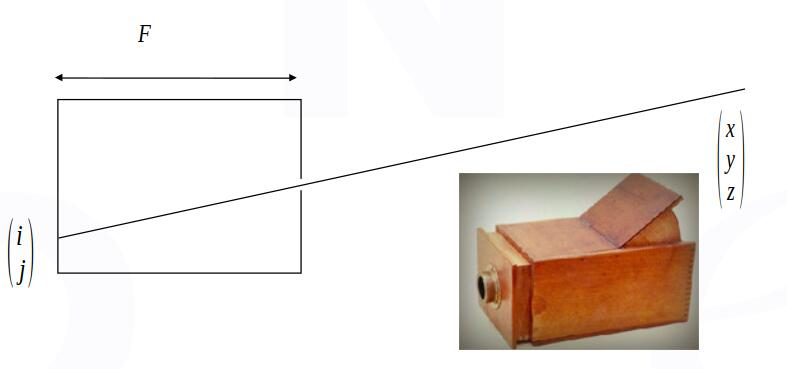
\includegraphics[width=12cm]{Methods/Images/CameraObscura.jpg}\caption{Camera osbcura : schema and a real object}
	\label{fig:CameraObscura}
\end{figure}


We begin by the description of very simple object, but which is really a the origin of
the photography and, in some way, is the simplest possible camera  :  the camera obscura.
Basically it can be described as a box with a hole, at the entrance of the box we have
a the hole that let the light in, and at the bottom of the box we have the film of
the camera. 

Figure~\ref{fig:CameraObscura} presents a real camera and a basic schema showing
the construction of the image :  to compute the image of a point $P^c=x^c,y^c,z^c$ of the real scene
we juts have to trace the line starting from $P^c$, going throw the hole and take its intersection $q=i,j$
with the image plane.


%-----------------------------------------------------
\subsection{Setting equations}

To compute a mathematical relation between $x^c,y^c,z^c$ and $i,j$ we will introduce several hypothesis 
and notations illustrated by figure~\ref{fig:Camera3DNote} :

\begin{figure}
\centering
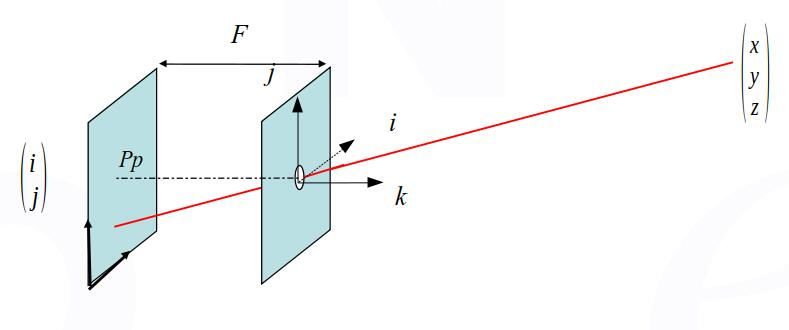
\includegraphics[width=12cm]{Methods/Images/Camera3D.jpg}\caption{Notation for camera relation}
	\label{fig:Camera3DNote}
\end{figure}

\begin{itemize}
	\item for 3d coordinates, we consider a local $3d$ repair $(O,\vec{i},\vec{j},\vec{k})$  where $O$ is the entrance hole,
              $\vec{i},\vec{j}$ belongs to the image plane and $\vec{k}$ is orthogonal to  $\vec{i}$ and $\vec{j}$;

	\item for $i,j$ we consider a image repair originated at one corner $c$ of the box;

	\item we note $P^p$ (principal point)  the intersection of axe $O\vec{k}$  with the image plane,
	      and $F$ (focal length) the distance between $P^p$ and $O$.

        \item we note $Q_3$  the $3d$ point corresponding to $q$.

\end{itemize}

To compute coordinates of $Q_3$ we can use chasles relation as indicated in equation~\ref{PC:Chasles} :

\begin{equation}
	\overrightarrow{OQ_3} =  \overrightarrow{O P^p} + \overrightarrow{P^p c} +  \overrightarrow{c Q_3}
	 =     \begin{pmatrix} 0\\0\\-F \end{pmatrix}
             + \begin{pmatrix} -P^p_x\\-P^p_y\\0 \end{pmatrix}
             + \begin{pmatrix} i\\j\\0 \end{pmatrix}
	 =     \begin{pmatrix} i-P^p_x\\j-P^p_y\\-F \end{pmatrix}
	\label{PC:Chasles}
\end{equation}

Now remind that light having a straight path, the $3$ point $Q_3$, $0$ and $P^c$ must be aligned,
which can be wrotten by equation~\ref{PC:Alignment} :

\begin{equation}
	\exists \lambda : 
	\begin{pmatrix} i-P^p_x\\j-P^p_y\\-F \end{pmatrix} 
      = \lambda   \begin{pmatrix} x^c\\y^c\\z^c \end{pmatrix}
		\label{PC:Alignment}
\end{equation}

By a simple quotient  we can elimimnate $\lambda$ in~\ref{PC:Alignment} and obtain :


\begin{equation}
	i = P^p_x -F \frac{x^c}{z^c}  \; ; \;
	j = P^p_y -F \frac{y^c}{z^c}  
	\label{PC:FormulaImaIntr1}
\end{equation}

%-----------------------------------------------------
\subsection{Local image formula}

The usage is to modiy the equation~\ref{PC:FormulaImaIntr1} by changing the sign of $F$;
this comes to consider a camera model ,
 not physically feasible and slightly different from the camera obscura,  
where the image plane is before the whole instead of behind, and that
is illustrated by figure~\ref{fig:PcInvCam}.  

\begin{figure}
\centering
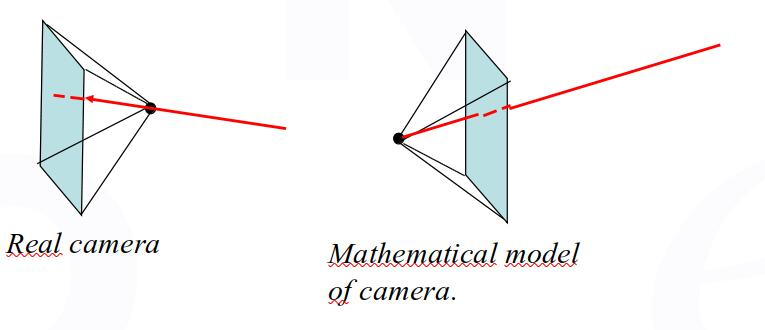
\includegraphics[width=12cm]{Methods/Images/InvCamera.jpg}
	\caption{Camera model : physically based one (left) and used one (right)}
	\label{fig:PcInvCam}
\end{figure}

Finally we will use equation~\ref{PC:FormulaImaIntr2} to formulate the relation between
local ground coordinates $P^c$  and image coordinate for this basic camera :

\begin{equation}
	i = P^p_x +F \frac{x^c}{z^c}  \; ; \;
	j = P^p_y +F \frac{y^c}{z^c}  
	\label{PC:FormulaImaIntr2}
\end{equation}

Setting the canonical projection $\pi_0$:

\begin{equation}
	  \pi_0 \begin{pmatrix} x^c \\ y^c \\ z^c \end{pmatrix} 
           =  \begin{pmatrix} \frac{x^c}{z^c} \\  \frac{x^c}{z^c}  \end{pmatrix} 
\end{equation}

and the intrinsic calibration $ \mathcal{I}_0$ :

\begin{equation}
	   \mathcal{I}_0  \begin{pmatrix} u \\  v  \end{pmatrix} 
		   =  P^p + F  \begin{pmatrix} u \\  v  \end{pmatrix}  \label{EqIntNoDist}
\end{equation}

we will write :

\begin{equation}
	q  =   \mathcal{I}_0 (\pi_0 (P^c))
\end{equation}


%-----------------------------------------------------
\subsection{Global image formula}

Generally we need to write the coordinate of $q$ as a function of the global coordinate $P$ or a point.
For this we just have to write the local coordinates $P^c$ as a function of global $P$, 
we use $C$ the center of the camera, and $R$ its orientation :

\begin{equation}
	P =  C+ R *P_c
\end{equation}

Which give the image formula :
\begin{equation}
	q  =   \mathcal{I}_0 (\pi_0 (^t R (P - C))) \label{FormImage0}
\end{equation}

This formula will follow us for a long time. The main thing that will evolve is $\mathcal{I}_0$,
and later $\pi_0$,
that will become more sophisticated to take into account lenses used in real camera.


%-----------------------------------------------------
\subsection{A remark on repair orientation}

We have not discussed untill now which image repair is used for image coordinates $i,j$.
The choice done in {\tt MMVII} is to use the native coordinate system of the image format,
knowing that majority of image format use a clockwise repair : 
that is : $i$ is left to right and $j$ is up to bottom (this is purely conventionnal, but one the
choice is made, is will have to be respected all along the process).

As we aline  local repair $(O,\vec{i},\vec{j},\vec{k})$  on this coordinate system ,
and we want a direct $3d$ repair with $\vec{k} = \vec{i} \wedge \vec{j} $, this
has for consequences that with these convention the axe $O\vec{k}$ is in the viewewing direction of the
camera.  The figure~\ref{fig:FormIm} illustrates this convention;


\begin{figure}
\centering
	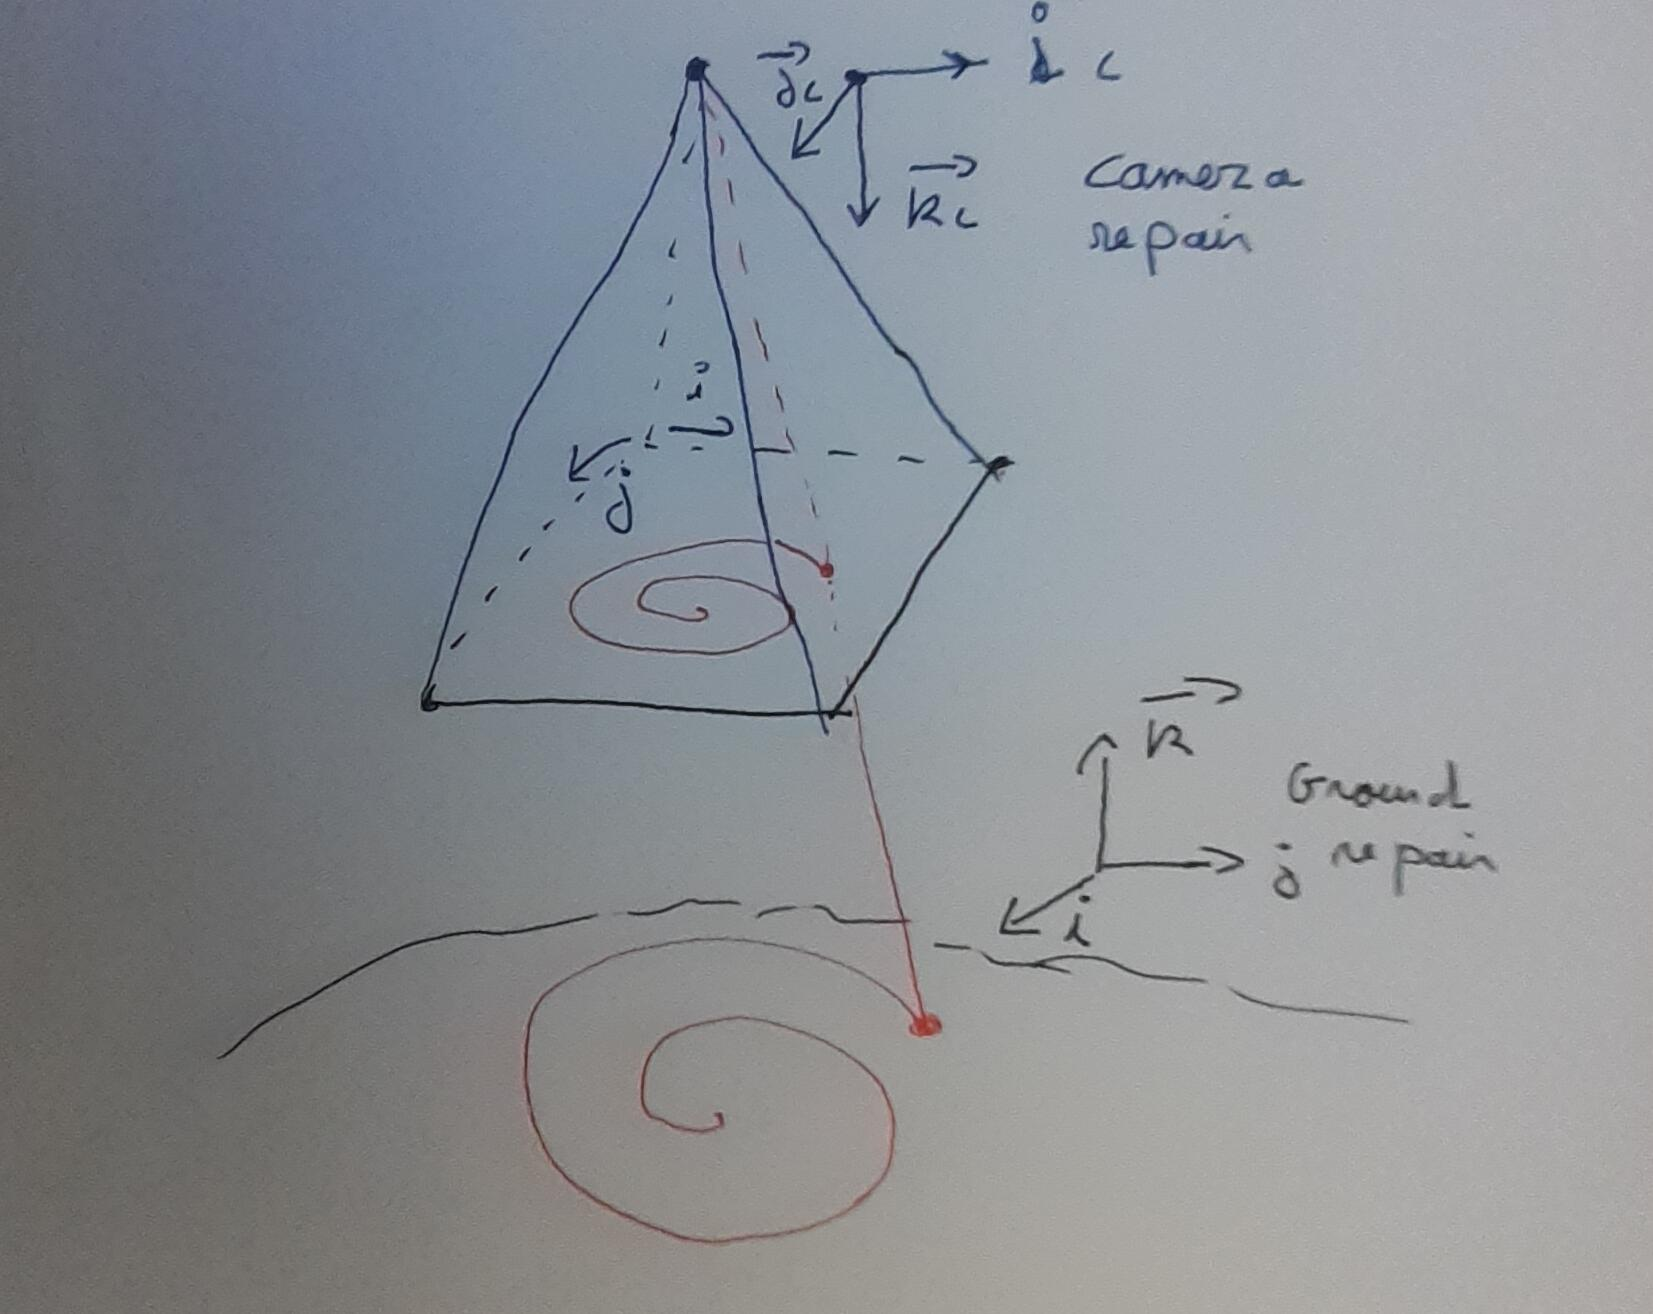
\includegraphics[width=12cm]{Methods/Images/RepairCam.jpg}
	\caption{Camera model : physically based one (left) and used one (right)}
	\label{fig:FormIm}
\end{figure}

%-----------------------------------------------------
%-----------------------------------------------------
%-----------------------------------------------------

\section{Beyond camera obscura}

%-----------------------------------------------------
\subsection{Need of lenses}

With the camera obscura, to have a sharp image we must keep a small entrance hole;
so to have enouh light we need very long exposure time (several hours). 
This is not convenient and the devlopment of photography
would not have been possible without the devlopment of optic. By puting a system
of lenses at the entrance of the system, and being caution that the  scene focalise
on the image plane, it was possible to have a sharp image whith a sufficiently big
hole and make photography practicable.

Nowday all the camera have more or less complicated system of lenses. In fact due the
automatization of the computer added conception they tend to be more and more complex, the concepter
using the possibility offered by multiple lenses with various materiel to correct more and more optical defaults .

For photogrammetry it change the game, because the lenses being not "infinitely thin", the gauss
condition non longer apply and some non linearity will occur , we will no longer be able to use
equation as simple as~\ref{EqIntNoDist} and will have to modelize accurately the effect of
lenses. 


%-----------------------------------------------------
\subsection{A parametric estimation issue}

A possible way to proceed would be to take into account the CAD plane of the optical
system, use in conception and to deduce the correction using the law of optic.  
Practically, we almots never proceed this way for two reasons  :

\begin{itemize}
   \item firt this CAD plane are rarely avalaible (maybe due to industrial property ?);
   \item second, and more important, the experience prove that when we proceed to the
         modelization of two lenses from the same model, we have to modelize them with two
         different parameter if we want to get the best accuracy, so no theoreticall model 
         would fit our requirement (also it could give a good first approximation);
\end{itemize}

So the approach currently used in photogrammetry is to select a parametric model
for the effect of lenses and to estimate the paramaters from the measures we have  (tie-point,
GCP, GNSS  \dots).


%-----------------------------------------------------
\subsection{Precaution to take}
\label{ParamFit}

\begin{figure}
\centering
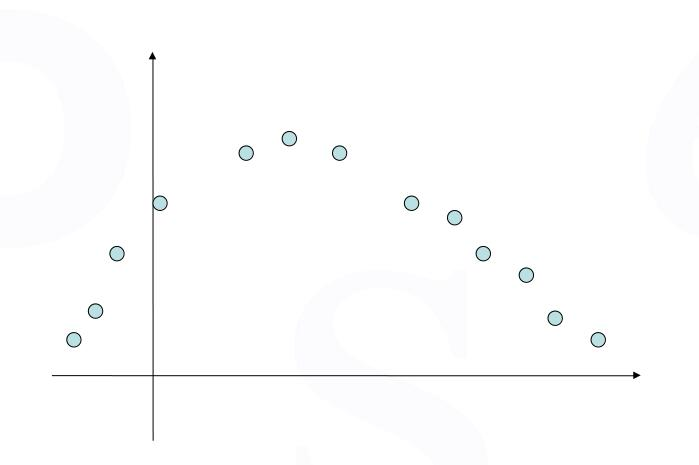
\includegraphics[width=6cm]{Methods/Images/Courbe-Pts.jpg}
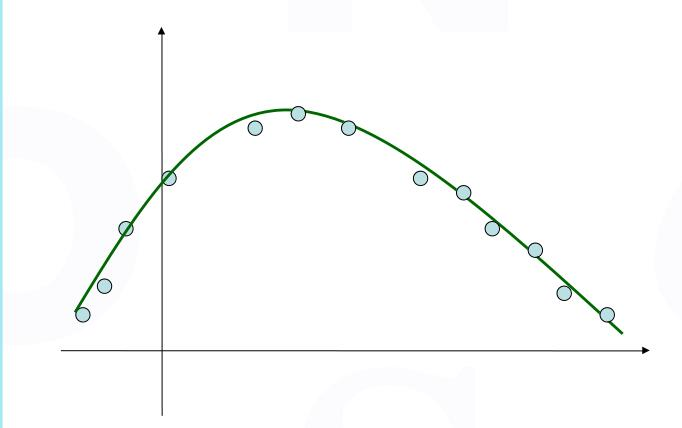
\includegraphics[width=6cm]{Methods/Images/CourbeGoodParam.jpg}\\
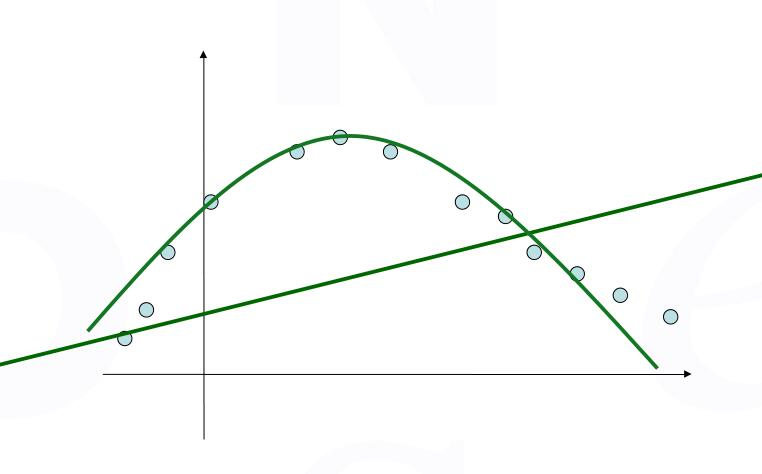
\includegraphics[width=6cm]{Methods/Images/Courbe-UndeParam.jpg}
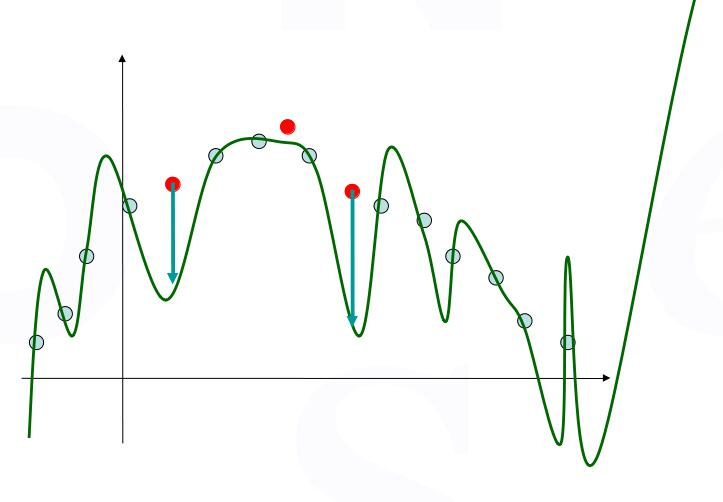
\includegraphics[width=6cm]{Methods/Images/CourbeOverParam.jpg}
	\caption{(1)Curves to interpolate (2) "Good" parametrization (3) Under parametrization (4) Over parametrization}
	\label{fig:CurvesParam}
\end{figure}


This empiricall approach does not prevent from being cautious
to the selection of model, we will have the usual compromise in the selection
of the parametric model, illustrated by figure~\ref{fig:CurvesParam}  on a problem of curve interpolation:


\begin{itemize}
	\item if we don't have enough parameters (curve 3) we are not accurate  even on the data to fit,
	   here if we fit with a straight line, or even with a parabol, we are not close to the learning data ;

   \item if we  have too many parameter (curve 4), we can have a very good match on the learning data, but have 
	 poor result as soon as we test with new data; this illustrated with  figure ??? were
         we use the "naive" lagrange interpolation to fit $N+1$ point with a $N$ degree polynomial,
         we have a perfect fit and the learning data, but due to high frequences a very poor fit outside;
\end{itemize}

The question of selecting the adequate model is a difficult one, and to our best knowledge
still open in photogrammetry.  Is it preferable to have over or under paramatrization ? There
exists controvorsery arguments :


\begin{itemize}
   \item  on one hand, as illustrated by figure ~\ref{fig:CurvesParam}, on can argue that under parametrization is less dangerous
         than over parametrization;

   \item  on the other hand, in "modern" photogrammetry the measurement comes more and more from automatic system,
          we can easily have several ten thousands of tie points, so one can argue that there is no real risk to have $100$ parameter
          even when we only really need $10$.
\end{itemize}

Consequently, it was thought, that the best we can do in {\tt MMVII} is to offer a sufficient large set of model
of camera, from the simple ones to the most universal one, and let the user select them according to
the precise knowledge of his domain. 

\begin{figure}
\centering
	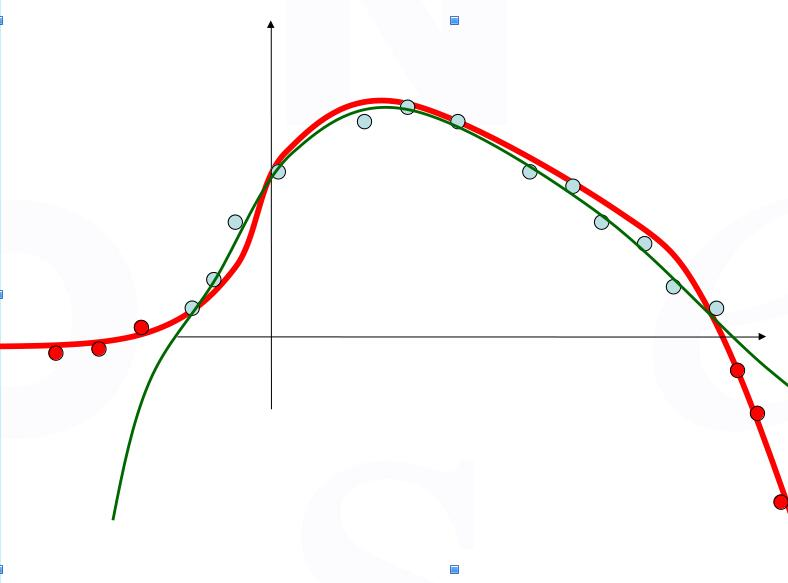
\includegraphics[width=6cm]{Methods/Images/CourbeExrapol.jpg}
	\caption{Extrapolation}
	\label{fig:CurvesExtrpol}
\end{figure}

However, even is this choice of parameter is not easy, there is
one universal rule : if we can be stable in interpolation, we are always bad in extrapolation
as illustrated on figure~\ref{fig:CurvesExtrpol}. A 
consequence when will estimate the model of a camera : if we have no measurement in the corners,
we are almost sure that we estimation will be poor in these corners.

%-----------------------------------------------------
\subsection{Still a central perspective, with a distorsion}
\label{Still:Persp}

In the next section we are going to introduce step by step, different model with a continuous
refinement of the physical modelization.  

\begin{figure}
\centering
	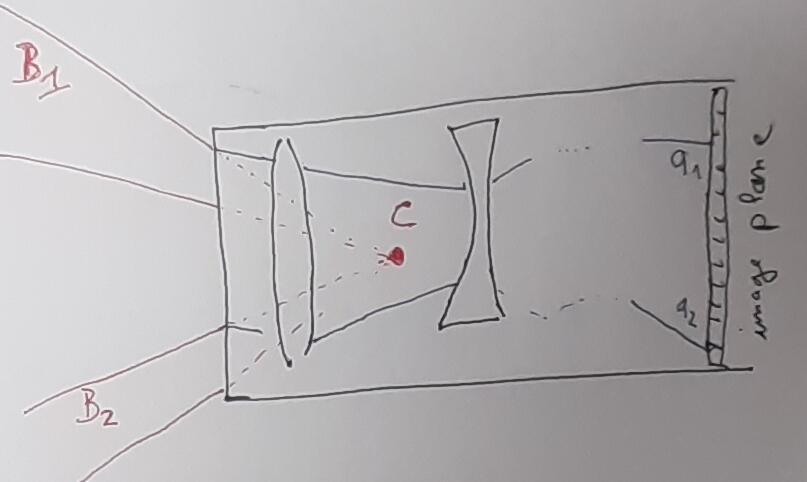
\includegraphics[width=8cm]{Methods/Images/CamPersp.jpg}
	\caption{Ligth path, all outing bundle converge to $C$}
	\label{fig:CamPerspScheme}
\end{figure}

The only hypothesis that we will maintain all allong these pages is that all the bundle issued from image
plane go through the same point $C$. This is schematised by figure~\ref{fig:CamPerspScheme} :
how complicated may be the ligth path inside the camera, we still have the property that
it exist a virtual point $C$, such that for any image point $q_i$, the bundle $B_i$ that lead to $q_i$
all go trough $C$.

This hypothesis is universally adopted, and justified because we still have a diaphragam that physicall contraint
the light to go trough it centers; of course the light will cross lenses before converning to this diaphragm but, 
, under gaussian approximation the image and reciproc image of converging bundle are still converging bundles.
To our knowledge, the only practicle cases where this hypothesis may be questionned are macro-photogrammetry and
sub-marine photogrammetry. We will discuss that ???. And maybe in the future of {\tt MMVII} project we will 
test option to relax this hypothesis for these context.

With this hypothesis, the image formation equation~\ref{FormImage0} still holds if
we add a supplentary $2d$ image deformation. Suppose in the initial simplistic camera
obscura, or even in a camera lenses satisfying gaussian approximation, 
the bundle $B_i$ would have arrived in $q^0_i$, now with the not thin lenses ,
it really arrive in $q_i$, we call $\phi$ the $2d$ mapping such that $\phi : q^0 \rightarrow q$.
With $ \mathcal{I}(q) = \phi (\mathcal{I}_0(q))  $, we have now :


\begin{equation}
	q  =   \mathcal{I} (\pi_0 (^t R (P - C)))
\end{equation}

By the way, for technicall reason we prefer to write : $ \mathcal{I}(q) = \mathcal{I}_0(D(q)) $ ; 
the reason being numericall stability of least square system, we prefer to have $D$ operate on adimentionnal numbers
(i.e as $\frac{x}{z}$).  The two modelization being obvioulsy equivalent from the pure mathematicall point of view :
as $D= \mathcal{I}_0^{-1} \circ \phi \circ  \mathcal{I}_0$.


%-----------------------------------------------------
\subsection{Summary : new image formula}

We note $D$ the additional term, classically named as distorsion. We assume for now that the 
system "almost" satisfies gaussian approximation ,  this is the case with standard lenses, 
and then $D$ can be assumed to be close to identity.
This will not be the case with fish-eye, and we will see that we will proceed by replacing $\pi_0$ by other
projection.

The following three equations summarize where we are in our modelization :



\begin{equation}
	q  =   \mathcal{I} (\pi_0 (^t R (P - C))) ; \label{FormImage1}
\end{equation}

\begin{equation}
	\mathcal{I} = \mathcal{I}_0  \circ D \label{FormImage2}
\end{equation}

\begin{equation}
	  D \approx Id \label{FormImage3}
\end{equation}

%-----------------------------------------------------
%-----------------------------------------------------
%-----------------------------------------------------

\section{Calibration as mapping "up to a rotation"}

\subsection{Introduction}

Before analysing the progressive refinement in modelisation of
distorsion, we  make a preliminary remark that is important
to avoid over parametrization (in fact , this over parametrisation
does not occurs this basic model described in~\ref{RadMod} or~\ref{DecMod}).


The function $\mathcal{I} \circ \pi_0$  of equation~\ref{FormImage1} can be seen as a function that
goes from the sphere of direction to the sensor.  In a first
step we will show that this determination of this function is intrinsequely ambiguous
\emph{up to a rotation} and then we will see the consequences.


\subsection{oo}

In equation ~\ref{FormImage1} , we note :

\begin{equation}
	P-C =  \overrightarrow{CP}  = \begin{pmatrix} x_c \\ y_c \\ z_c \end{pmatrix} 
\;\;\;  ;  \;\;\;
        ^t R =  \begin{pmatrix}  A & B & C \\ D & E & F \\ G & H & I \end{pmatrix} 
\end{equation}

Now we have in equation~\ref{DecMod} :

\begin{equation}
	\pi_0(^t R(\overrightarrow{CP})) 
	=  \frac{\begin{pmatrix} Ax_c+By_c+Cz_c \\ Dx_c+Ey_c+Fz_c  \end{pmatrix}}{Gx_c+Hy_c+Iz_c}
		=  \frac{\begin{pmatrix} A\frac{x_c}{z_c}+B\frac{y_c}{z_c}+C \\  D\frac{x_c}{z_c}+E\frac{y_c}{z_c}+F  \end{pmatrix}}
			{G\frac{x_c}{z_c}+H\frac{y_c}{z_c}+I}
\end{equation}

Let note $H_R$ the $2D$  homography defined by :

\begin{equation}
  \mathcal{H}_R(u,v) =  \frac{\begin{pmatrix} Au+Bv+C \\  Du+Ev+F  \end{pmatrix}} {Gu+Hv+I}
\end{equation}

We then have :

\begin{equation}
	\pi_0(^t R(\overrightarrow{CP}))  = \mathcal{H}_R  (\pi_0 (\overrightarrow{CP}))
\;\;\;  ;  \;\;\;
        \pi_0  \trans  R = \mathcal{H}_R  \pi_0
\end{equation}

We now go back to equation~\ref{FormImage1}, and for any rotation $R'$, we insert it using $^t R'R'=Id$ :

\begin{equation}
	\mathcal{I} \pi_0   \trans R = \mathcal{I}  \pi_0   (\trans R' R')  \trans R = ( \mathcal{I}  \pi_0   \trans R')  (R' \trans R )
\end{equation}

Or :

\begin{equation}
	   \mathcal{I} \pi_0   \trans R 
	   = (\mathcal{I} \mathcal{H}_{R'})   \pi_0   \trans (R \trans R')  \label{FormRotCalib}
\end{equation}


%-----------------------------------------------------
%-----------------------------------------------------
%-----------------------------------------------------

\section{Radial modelisation}

\label{RadMod}

In this section we  show that the radial modelisation of distorsion is a consequence
of the hypothesis of cylindric symetry of the optical system.

%--------------------------------------------------------------------------------------------------------

\subsection{Radial symetry hypothesis}

\begin{figure}
\centering
	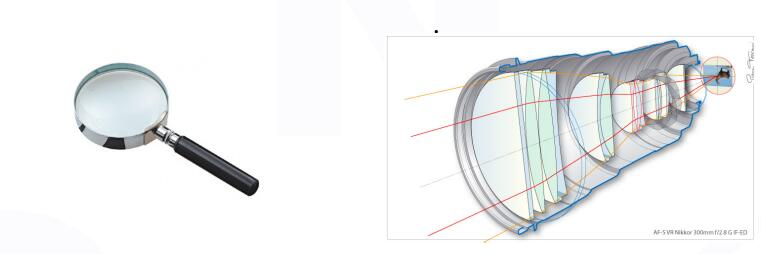
\includegraphics[width=12cm]{Methods/Images/Lenses.jpg} \\
	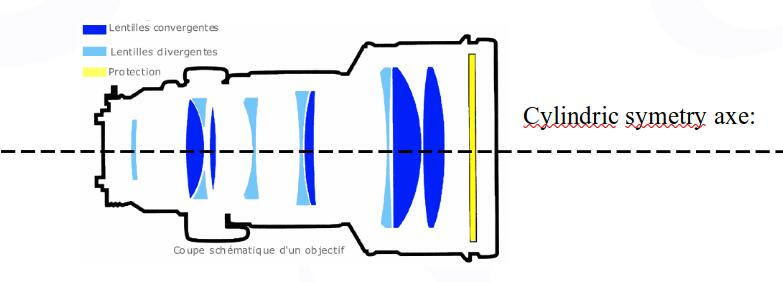
\includegraphics[width=8cm]{Methods/Images/LensesCyl.jpg}
	\caption{A single lense , and modern }
	\label{fig:Lenses}
\end{figure}

We start the modelization with three observations on the theoreticall design of central perspective cameras:

\begin{itemize}
    \item  each individual lense has a radial symetry arround it opticall axe;:
    \item  the mechaninal building is made so that all the lenses are aligned on
	    their common optical axe $\mathcal{A}$.
    \item  the plane of the sensor is orthognal to $\mathcal{A}$.
\end{itemize}

For real camera, these observation are satisfied with a high accurracy in the sense that it is
rigourously satisfied in the theoreticall conception model of almost all central perspective
camera~\footnote{to our knowledge the only notable exception if tilt lenses, for the orthogonality rule}.
Consequently all the corrective terms that we will study in further sections,
are due to the difference between theoreticall model and effective realization and are
generally of an order of magnitude lower than the radial distorsion.

These elementary remarks have for consequence that, how sophisticated may be the combination
of many lenses, each having a complicated non spherical shape, we still have a global cylindrical
symetry on our system. This is illustrated by schemes of figure~\ref{fig:Lenses}.
The perspective center $C$ defined in \ref{Still:Persp}, must belong to the axes of symetry,
so we have $\mathcal{A}=(C,\vec{k})$. 

%--------------------------------------------------------------------------------------------------------

\subsection{Notation}

For a direction of vector we will use spherical coordinates in repair $\vec{i},\vec{j},\vec{k}$ :

\begin{equation}
	\vec{S_{ph}}(\theta,\phi)   =\begin{pmatrix}  \cos(\theta) \sin(\phi) \\ \sin(\theta) \sin(\phi)  \\ \cos(\phi) \end{pmatrix}
	     \label{PC:Spher:Coord}
\end{equation}

We  note $\mathcal{P}_{\theta}$  the plane passing by $\mathcal{A}$ and containing the vector    $\vec{S_{ph}}(\theta,.)$
(the $.$ enhances that whatever may be the value $\neq 0$ , it will define the same plane).

For any ray intersecting $\mathcal{A}$, we will note $R(z,\theta,\phi)$ the ray of direction $\vec{S_{ph}}(\theta,\phi)$  crossing $\mathcal{A}$
at abscissa $z$  :

\begin{equation}
	R(z,\theta,\phi) = \{C+ z \vec{k} + \lambda \vec{S_{ph}}(\theta,\phi), \lambda \in \RR\}
	     \label{PC:RayParam}
\end{equation}


%--------------------------------------------------------------------------------------------------------

\subsection{Intuitive formulation}

Let $B$ be an incoming ray, noted $ R(0,\theta,\phi)$ , let $B'$ be the outcoming ray  that will intersect the sensor,
we want to establish the property of the transformation  $ \Psi : B \rightarrow B'$.
If we admit the \emph{intuitive} following proposals :


\begin{proposal}[3D radial symetry-physicall modelization]  \;
\label{PhysRadMod}
\begin{enumerate}
    \item  $\Psi$ is globally stable inside any plane  $\mathcal{P}_{\theta}$; \label{PhysRadModPlane}

    \item  any  circular cone $\mathcal{C}$ of bundle  arround $\mathcal{A}$ is
	    transformed by $\Psi$ in another circular cone arround $\mathcal{A}$  (but possibly with a different origin and angle);
\end{enumerate}
\end{proposal}

This has for consequence that , noting  $B'=(z',\theta',\phi')$ \footnote{which is possible because $B'$ intersect  $\mathcal{A}$ due to first proposal},
we have : (1) $\theta'=\theta$  (2)  $z'$ and $\phi'$ depends only of $\phi$. 
Then $\Psi $ has the following parametric form, where $\zeta$ and $\Phi$ are mapping $\RR \rightarrow \RR$ :

\begin{equation}
	\Psi(B) = \Psi(R(0,\theta,\phi)) = R(\zeta(\phi) ,\theta,\Phi(\phi))
\end{equation}

Next section is a formal proof,  it can be omited by the reader in a hurry who is already conviced of the above proposal.


%--------------------------------------------------------------------------------------------------------

\subsection{Proof}

\begin{figure}
\centering
	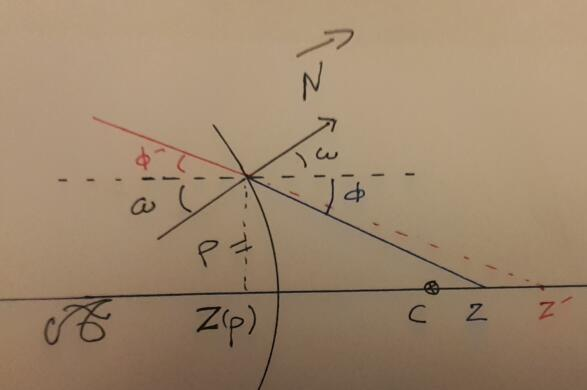
\includegraphics[width=12cm]{Methods/Images/Radial-PhiOmegaZ.jpg} \\
	\caption{Notation for dioptr crossing}
	\label{fig:RadPhiOmegZ}
\end{figure}

The optical system is made of succession of diopters $D_1,\dots D_n$,
that are have all a symetry arround $\mathcal{A}$.  Noting $\Psi_k$
the elementary transformation by a single dioptr  we will  proof ;

\begin{proposal}[3d radial symetry of dioptr]  \;
If  we have a set of ray $R(z,\theta,\phi)$ intersecting  $\mathcal{A}$ such that  z is function of $\phi$ :
$z=\zeta(\phi)$, then  all the output ray satisfy the same property ; they intersect $\mathcal{A}$ and there exist 
two mappings  $\RR \rightarrow \RR$ , $\zeta'$ and $\Phi'$  such:

\begin{equation}
	\Psi(B) = \Psi(R(\zeta{\phi},\theta,\phi)) =  B' = R(\zeta'(\Phi'(\phi)),\theta,\Phi'(\phi))
\end{equation}
\end{proposal}

As the condition \emph{"x is function of $\phi$"} obviously applies for initial rays (i.e. $x=0$ for all as they cross $C$),
we will have proven what we want as $\Psi = \Psi_n \circ  \Psi_{n-1} \circ \dots \circ \Psi_1$. Note also that the requirement
for initial ray is a bit more general than imposing that all ray cross $C$, it is sufficient that they complies with requirement
of proposal above (intersect $\mathcal{A}$ and abscissa of intersection depends only of $\phi$).


We will use cylindric coordinate $\rho,\theta,z$ arround $\mathcal{A}$, where $\theta$ is the same than the spherical
coordinate used in equation~\ref{PC:Spher:Coord}

\begin{equation}
	C_{yl}(\rho,\theta,z)   =\begin{pmatrix} \rho \cos(\theta)  \\ \rho \sin(\theta)   \\ z \end{pmatrix}
	     \label{PC:Cyl:Coord}
\end{equation}

Consider a ray $B$ that is deflected in $B'$ when it meets the dioptr  $D$ in point $P$.
The surface of the dioptr $D$, can be caraterized by the equation $z=Z(\rho,\theta)$, and due to cylindric symetry we have in fact :
$z=Z(\rho)$.  We can then establish a parametric representation of the surface :

\begin{equation}
	Q(\rho,\theta) =  C_{yl}(\rho,\theta,Z(\rho,\theta)) = \begin{pmatrix} \rho \cos(\theta)  \\ \rho \sin(\theta)   \\ Z(\rho) \end{pmatrix}
\end{equation}

The normal $\vec{N}(\rho,\theta) $ to the surface can be computed as :


\begin{equation}
	\vec{N}(\rho,\theta) 
	=  \frac{\partial Q}{\partial \rho} \wedge \frac{\partial Q}{\partial \theta}
	=   \begin{pmatrix} \cos(\theta)  \\  \sin(\theta)   \\    \frac{\partial Z}{\partial \rho}   \end{pmatrix}
            \wedge 
	   \begin{pmatrix} -\rho \sin(\theta)  \\ \rho \cos(\theta)   \\ 0 \end{pmatrix}
	=   \begin{pmatrix}  - \rho \frac{\partial Z}{\partial \rho}  \cos(\theta)  \\  -\rho \frac{\partial Z}{\partial \rho}  \sin(\theta)   \\  \rho     \end{pmatrix}
	=   \begin{pmatrix}  0 \\  0 \\  \rho     \end{pmatrix}
            - \rho \frac{\partial Z}{\partial \rho}   \begin{pmatrix}   \cos(\theta)  \\   \sin(\theta)   \\  0     \end{pmatrix}
		    \label{PC:EqNorm}
\end{equation}

Equation~\ref{PC:EqNorm} shows that the normal  $\vec{N}(\rho,\theta)$ belongs to plane $\mathcal{P}_{\theta}$. 
So as $\vec{N}(\rho,\theta)$ and $\vec{B}$  belongs to $\mathcal{P}_{\theta}$ , first Snell-Descartes law on refraction 
implies that  $\vec{B'}$ belongs also to  $\mathcal{P}_{\theta}$.  This proves the first
that $B' \subset  \mathcal{A}$ and $\theta'=\theta$.

Let write $\vec{N} = S_{ph}(\theta,\omega)$ as illustrated on  figure ???;  due to radial symetry  ,
$\omega$ does not  depends of $\theta$ (see also equation~\ref{PC:EqNorm} : $\tan(\omega)= \frac{\partial Z}{\partial \rho}$) :  $\omega$  depends only of $\phi$.
So using Snell-Descartes law on refraction gives, noting $n$ the reflexion indice after $D_k$, we have :

\begin{equation}
	n'  \sin(\omega + \phi') = n  \sin(\omega + \phi)
\end{equation}

This proves that $\phi'$ is a function of $\phi$ :  $\phi' = \Phi(\phi)$.

Also we have  :


\begin{equation}
	\sin(\phi) = \frac {z-Z(\rho) }{\rho}
	\label{Eq:PhiZRhoIn}
\end{equation}
\begin{equation}
	\sin(\phi') = \frac {z'-Z(\rho) }{\rho}
	\label{Eq:PhiZRhoOut}
\end{equation}

Equation \ref{Eq:PhiZRhoIn} show that $\rho$ is a function of $\phi$  and $z$, then $\rho$ is a function of $\phi$ (as $z$ is function of $\phi$).
Equation \ref{Eq:PhiZRhoOut} show $z'$ is a function of $\rho$ and $\phi'$, but $\rho$ is a function of  $\phi$ and
then a function of $\phi'$  ($\phi = \Phi^{-1}(\phi')$).


%--------------------------------------------------------------------------------------------------------

\subsection{Radial distorsion in the plane}

\begin{figure}
\centering
	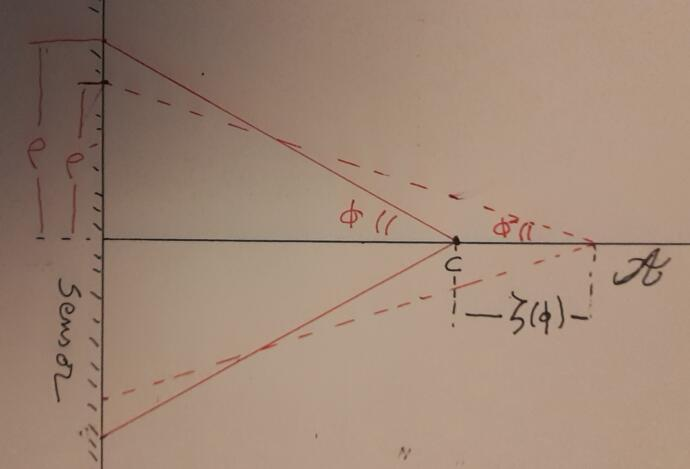
\includegraphics[width=12cm]{Methods/Images/RadialInThePlane.jpg} \\
	\caption{Notation radial distorsion}
	\label{fig:RadInPlane}
\end{figure}

Untill now, we have computed the distorsion in $3d$ as a function $\Psi$ modifying the path of light. To use 
equations~\ref{FormImage1} and~\ref{FormImage2} we need to convert the effect $\Psi$  in image plane.
We use notation of figure~\ref{fig:RadInPlane}.


Without distortion the ray will arrive at point $q$  given by :

\begin{equation}
	q =     \begin{pmatrix} P^p_x \\ P^p_y \end{pmatrix} +  F \tan(\phi)   \begin{pmatrix} \cos(\theta) \\ \sin(\theta) \end{pmatrix} 
\end{equation}

With distorsion, the ray will arrive at point $q' = D(q)$ given by :

\begin{equation}
	q' =     \begin{pmatrix} P^p_x \\ P^p_y \end{pmatrix} +  (F+z') \tan(\phi')   \begin{pmatrix} \cos(\theta) \\ \sin(\theta) \end{pmatrix} 
		=     \begin{pmatrix} P^p_x \\ P^p_y \end{pmatrix} +  (F+\zeta(\Phi(\phi))) \tan(\Phi(\phi))   \begin{pmatrix} \cos(\theta) \\ \sin(\theta) \end{pmatrix} 
\end{equation}

Using polar coordinates arround $P^p$ we have :

\begin{equation}
	q = P^p + P_{ol}(\rho,\theta) =  P^p+  P_{ol} ( F \tan(\phi), \theta) \label{PolInit} 
\end{equation}

\begin{equation}
	q' = P^p+   P_{ol}(\rho',\theta) =  P^p+  P_{ol}( (F+\zeta(\Phi(\phi))) * \tan(\Phi(\phi)), \theta) \label{PolDist}
\end{equation}

So : 

\begin{equation}
       \rho = F \tan(\phi)   \;\;\; , \;\;\;  \rho' = (F+\zeta(\Phi(\phi))) * \tan(\Phi(\phi))   \label{RhoPhi}
\end{equation}

We see that $\rho$ and $\rho'$ are both function of $\phi$, this show that $\rho'$ can be
computed as a function of $\rho$ (just replace $\phi$ by $\tan^{-1}(\frac{\rho}{F})$ in  $\rho'= (F \tan(\phi) +\zeta(\Phi(\phi))) * \tan(\Phi(\phi))$,
\footnote{but the exact formula istself is not important}).
The distorsion $D : q \rightarrow q' $ can then be completely caracterized by the radial distorsion
$D_r : \rho \rightarrow  \rho'$ :

\begin{equation}
	D(q)  =   D(P_{ol}(\rho,\theta))  =   P_{ol}(D_r(\rho),\theta)
\end{equation}

%--------------------------------------------------------------------------------------------------------

\subsection{Polynomial radial distorsion in polar coordinate}

The three point important in formula~\ref{RhoPhi} and the consequence for $D_r$  are :

\begin{itemize}
   \item $\rho$ and $\rho'$ can be computed as \emph{smooth} function of $\phi$; in fact we can 
         consider that the lenses have $\mathcal{C}^{\infty}$ shape ,  then   $\rho$ and $\rho'$ 
         are $\mathcal{C}^{\infty}$ are functions of $\phi$ , and finally $\rho'$ is a 
         $\mathcal{C}^{\infty}$ function $\rho$;

   \item for standard optics we have  $\zeta \approx 0$ and $\Phi \approx Id$,  then we have $D_r \approx Id$;
         by standard standard optics we mean optics where lenses are relatively thin, then  we are not far from Gauss approximation,
         this hypothesis do not hold for fish-eye lenses and we will rediscuss that in section~\ref{SecFE};

   \item $\rho$ and $\rho'$ are  \emph{odd}  function of $\phi$ , and then $\rho'=D_r(\rho)$ is as an \emph{odd}  function of 
        $\rho$;

\end{itemize}

As a synthesis :

\begin{proposal} \;
\label{DrHyp}
       $D_r$ is $\mathcal{C}^{\infty}$, odd function close to identity.
\end{proposal}

For justifying the polynomial approximation of $D_r$, we can then use a classical result of function 
approximation, the Stone-Weierstrass theorem (\cite{Weierstrass1885} and \cite{Stone1937})
which say that the space of polynoms is dense in the space of continuous function on closed bounded set;
so with a sufficient degree the function can be approximated as close as we want by a polynom.
Which lead to the parametric formula for $D_r$ and $D$ :

\begin{equation}
	D_r(\rho)  =   \rho  * (k_0 + k_1 \rho^ 2 + k_2 \rho^4 \dots  + k_n \rho^{2n})
\end{equation}

This formula require several comment :

\begin{itemize}
    \item  as $D_r$ is an odd function, we have only odd degree for polynom ; 

    \item  in the next we will set $k_0=1$, as the variation on scale are already handled by focal;
\end{itemize}

%--------------------------------------------------------------------------------------------------------

\subsection{Polynomial radial distorsion in euclidean coordinates}

Also polar coordinate are convenient for modelization of phenomena with radial symetry, 
they are not ideal for computation : they are relativelly slow and  the center point is
a critical point that can complexify some equation.  Sometime we cannot avoid them
easily, but here it happens that we can express w/o problem the distorsion
with euclidean coordinates:

\begin{equation}
\begin{multlined}
D(q)  =   P_{ol}(\rho  * (1 + k_1 \rho^ 2 + \dots) ,\theta)  \\
=   (1 + k_1 \rho^ 2 +  k_2 \rho^ 4 \dots)  \begin{pmatrix} \rho\cos(\theta) \\ \rho \sin(\theta) \end{pmatrix} \\
=   (1 + k_1 (x^2+y^2) +  k_2 (x^2+y^2) ^2 \dots)  \begin{pmatrix} x \\ y \end{pmatrix}
\end{multlined}
\end{equation}



%--------------------------------------------------------------------------------------------------------

\subsection{Variations on  conventions on radial distorsion}

As often in photogrammetry, there are many conventions and options for representing the same thing,
or small variations on the same things, in different book, papers, software \dots
We discuss here some of this options.

  % -  -  -  -  -  -  -  -  -  -  -  -  -  -  -

\subsubsection{Order of combinaison}

In previous section, in equation~\ref{FormImage2}, we have written  $ \mathcal{I} = \mathcal{I}_0  \circ D \label{FormImage2}$.
In several software the order of combination is invert of this one and authors use instead:

\begin{equation}
	\mathcal{J} = D \circ  \mathcal{I}_0  
\end{equation}

First we can remark that from the mathematicall point of view, the two convention are equivalent in the sense
that they define the same space of function.  With first convention we have :

\begin{equation}
	\mathcal{I}(q) = P^P + F (1 + k_1 (x^2+y^2) +  k_2 (x^2+y^2) ^2 \dots)  \begin{pmatrix} x \\ y \end{pmatrix}
\end{equation}

With second convention , as we operate on pixel the center of radial symetry will  be $P^p$ 
(althouh with "our" convention it is implicitely $0,0$). For the radial distorsion 
we compute first  $  \mathcal{I}_0 : q \rightarrow  P^p + F*q$, then we substract 
$P^p$  who is the center of distorsion, and obtain the formula :

\begin{equation}
	\mathcal{J}(q) = P^P + (1 + K_1 F^2 (x^2+y^2) +  K_2  F^4 (x^2+y^2) ^2 \dots)  \begin{pmatrix} F*x \\ F*y \end{pmatrix}
\end{equation}

So we see that they are equivalent and the conversion is here relatively easy  $K_1 = \frac{k_1}{F^2} $,
$K_2 = \frac{k_2}{F^4} $ \dots

This show  that there is no "hard" reason for selecting one convention to the other. The reason for
prefering convention  $\mathcal{I}_0  \circ D$ was :

\begin{itemize}
    \item some \emph{a priori} preference for numbers without unity;

    \item coefficient easier to interpret (typically, on realistic example, between $10^{-1}$ and $10^{-3}$ rather than between $10^{-8}$ and  $10^{-27}$)

    \item \emph{a priori} better for numerical stability.
\end{itemize}

  % -  -  -  -  -  -  -  -  -  -  -  -  -  -  -

\subsubsection{Names of coefficients}

In computer vision, the coefficient are name $k_1$, $k_2 \dots$ 
In  "traditionnal" photogrammetry, they are often named $R_3,R_5,R_7\dots$.

  % -  -  -  -  -  -  -  -  -  -  -  -  -  -  -

\subsubsection{Degree of polynon}

There is the question of what is the desirable degree of $n$, this is related to the general question issued in~\ref{ParamFit}
and there is no universal answer;  the "tradition" of aerial photogrammetry is to restrict to $n=3$  (i.e. $R_3,R_5,R_7$),
the "tradition" in computer vision is often to restrict to $n=2$, or even $1$;  also with modern lenses and modern
process there is argument for having higer degree  :
           
\begin{itemize}
         \item   with automatic tie point, we have currently several thousand measurement, the risk of over parametrisation
                 with $n=5$ , or even $10$ is low;

         \item   with automatic tie point, we have currently several thousand measurement, the risk of over parametrisation
\end{itemize}

  % -  -  -  -  -  -  -  -  -  -  -  -  -  -  -

\subsubsection{PPA and PPS}

In aerial photogrammetry, the "tradition" is to consider that the center of symetry of radial distortion
is different of principal point; they are named PPA (principal point of autocolimation) and
PPS (principal point of symetry).

We dont do it in {\tt MMVII} because it woul be redundant we other parameters 
selected as discussed in detail in \label{PPA:PPS:DEC}.
This is why in previous section we have used $P^p$ the center of symetry of the distorsion 
(in fact $0,0$ with our conventions).

%-----------------------------------------------------
%-----------------------------------------------------
%-----------------------------------------------------

\section{Decentric distorsion}
\label{DecMod}

\subsection{Introduction}
The previous section has establish the radial distorsion, that would almost always
be sufficient if the physical camera was a perfect realization of the designed camera.
In the next section we will discuss the main "default" in the realisation of
the camera and the additional parameters that are added to modelize them.

The first hypothesis  that will be questionned is the fact that the axes of the different
lenses are perfectly aligned.

%-----------------------------------------------------
\subsection{Mathematicall modelisation}

First we must translate in mathematicall terms the physicall words
"the lenses are slightly miss aligned".
We will do it by  the following assumption :

\begin{itemize}
    \item  each of the $N$ elementary block of well alligned lenses can still be 
           modelized by a central distorsion $D^k$ of centre $C^k$ and radial
           disorsion $D^k_r$;

    \item  the globall distorsion is the composition of the elementary distorsion
           $ D = D^1 \circ D^2 \circ \dots \circ D^n$

    \item  all the elementary distorsion are close to identidy, what we write :
           $D^k = Id + \delta^k$  with $\delta^k \approx 0$;

    \item  all the center of symetry are close to each others , and for simplicity
           we will write $C_k \approx (0,0)$;
\end{itemize}


We first need to show that $D^1 \circ D^2  \approx Id + \delta_1 + \delta_2$ up to second order term.
We will write $A\ll B$ for A is negligible with respect to B. We write $\nabla_F$
the jacobian of $F$, we have the taylor expansion :

\begin{equation}
	F(x+d_x) = F(x) + \nabla_F d_x + \epsilon(|d_x|) |d_x|  \;\; ; \;\;  \epsilon(|d_x|) \ll 1
\end{equation}


Consider now two function close to identity $D^1$ and $D^2$, we can write :
\begin{equation}
\begin{multlined}
(D^1 \circ D^2)(p)  \\
=  (Id+\delta^1)(p+\delta^2(p))\\
=  p +\delta^2(p) + \delta^1(p+\delta^2(p)) \\
=  p +\delta^1(p) + \delta^2(p) + \nabla_{\delta^1} \delta^2   + \epsilon(\delta^2(p)) |\delta^2(p)|
\end{multlined}
\end{equation}

For a firts order approximation of last line :

\begin{itemize}
   \item we have $\epsilon(\delta^2(p)) |\delta^2(p)|  \ll |\delta^2(p)|$ because $\epsilon\ll 1$,
          and this term can be neglected at first order;

   \item  for  $ \nabla_{\delta^1} \delta^2$ , it's less obvious, we admit here that
          if $\delta^1 \ll 1$ then $ \nabla_{\delta^1} \ll 1$,  in fact say like w/o further hypothesis this
		is wrong \footnote{consider for example $x^2 sin(\frac{1}{x})$, but its not $\mathcal{C}^\infty$}, but it becomes
          true if we add the condition that $\delta^1$ is smooth, however this would take us too far  and we admit it;
\end{itemize}

We have shown that $D^1 \circ D^2  \approx Id + \delta_1 + \delta_2$ .  Now it's trivial by recurence to
show that :

\begin{equation}
     D^1 \circ D^2   \dots D^n  \approx Id + \delta^1 + \delta^2 \dots + \delta^n
\end{equation}

%-----------------------------------------------------

\subsection{$2$ block case}

Consider now $D_1$ and $D_2$ two  radial distorsion; using center $C_k$, let write :

\begin{itemize}
	\item $\vec{u}_k = \overrightarrow{C_k p} = ^t (x_k,y_k) $ the vector joining $C_k$ to $p$;
	\item $R_k = ||\vec{u}_k||^2$  the square of the norm of $\vec{u}_k$ (i.e.  square of $\rho_k$ in radial coordinates) ;
\end{itemize}


Using the polynom  of distorsion $D^k_r(R) = k^k_1 R + k^k_2 R^2  \dots$  , we can write :
\begin{equation}
	\delta^k(p) =   D^k_r(R_k) \vec{u}_k 
\end{equation}

Then :

\begin{equation}
\begin{multlined}
	D^1 \circ D^2 (p)  \\
	= p +\delta^1(p) +\delta^2(p) \\
	= p +    D^1_r(R_1) \vec{u}_1  +  D^2_r(R_2) \vec{u}_2  \\
\end{multlined}
\end{equation}

As the two distorsions have close centers, even if their polynom of distorsion funcion are very different,
we can expect that each is close to a radial distorsion with the center of the other.
So we take arbitray one of both as the "reference, here  $D_1$,
and we write $D_2$ as a distorsion around the $C_1$ with polynom of $D^2_r$  plus an corrective term :

\begin{equation}
	\delta^2(p) =   D^r_2(R_1) \vec{u}_1  + ( D^2_r(R_2) \vec{u}_2 - D^2_r(R_1) \vec{u}_1 )
\end{equation}

In this equation the first term is a radial distorsion of center $C_1$. For the second term,
consider the function $\vec{\delta_2}$ defined by :

\begin{equation}
	\vec{\delta^2}(\vec{u}) =  D^r_2(||\vec{u}||^2) \vec{u}
\end{equation}

We can write the second term as :

\begin{equation}
	\vec{\delta^2}(\vec{u_2})  - \vec{\delta^2}(\vec{u_1})
\end{equation}

This term, can then be seen as the difference of the values of function $\vec{\delta^2}$, between $\vec{u_2}$
and $\vec{u_1}$.  But $\vec{u_2}$ and $\vec{u_1}$ are close because
$C_1$ and $C_2$ are. So we can approximate this term with  a Taylor expansion :

\begin{equation}
	\vec{\delta^2}(\vec{u_2})  - \vec{\delta^2}(\vec{u_1})
	\approx
	(C^2_x - C^1_x) \frac{\partial{\vec{\delta^2}}}{\partial x} (\vec{u_1})
     + 	(C^2_y - C^1_y) \frac{\partial{\vec{\delta^2}}}{\partial y}  (\vec{u_1})
\end{equation}

Note that we have used $\vec{u_1}$ as value where the devlopment is made, we could have used $\vec{u_2}$,
it's arbitrary and they are close.
So, merging previous equation, we can write :

\begin{equation}
	D^1 \circ D^2 (p) 
	\approx
	  p +    (D^1_r(R_1) + D^2_r(R_1))  \vec{u}_1  
	  +  \Delta_x \frac{\partial{\vec{\delta^2}}}{\partial x} (\vec{u_1})
          +  \Delta_y \frac{\partial{\vec{\delta^2}}}{\partial y}  (\vec{u_1})
\end{equation}

The term $(D^1_r(R_1) + D^2_r(R_1))  \vec{u}_1 $ is a pure radial term 
(with center $C_1$).    The second term is the "decentric" term itself.
To keep it simple, we will adopt the usual implicit convention for this term,
we limit the radial distosion to the first term $k_1 \rho_1^2$; note that {\tt MMVII} allow to use 
abitrary number of term .  So we have

\begin{equation}
\begin{multlined}
	\vec{\delta^2} (\vec{u_1}) = k_1(x_1^2+y_1^2)  \begin{pmatrix} x_1  \\ y_1 \end{pmatrix} \\
%
		\frac{\partial{\vec{\delta^2}}}{\partial x} 
		=  k_1 \begin{pmatrix} 3 x_1^2 + y_1^2    \\ 2 x_1 y_1  \end{pmatrix}
%
			\;\;\;\;   ; \;\;\;\;   
		\frac{\partial{\vec{\delta^2}}}{\partial y} 
		=  k_1 \begin{pmatrix} 2 x_1 y_1 \\ x_1^2 + 3 y_1^2  \end{pmatrix}
\end{multlined}
\end{equation}


Using standard convention, we name $\alpha = k_1  \Delta_x $ and $\beta = k_1  \Delta_y$;

\begin{equation}
	D^1 \circ D^2 (p) 
	\approx
	= p +    (D^1_r(R_1) + D^2_r(R_1))  \vec{u}_1  
	  +\begin{pmatrix} \alpha(3 x_1^2 + y_1^2 ) +2\beta x_1 y_1   \\ 2  \alpha x_1 y_1 +  \beta( x_1^2 + 3 y_1^2)  \end{pmatrix}
\end{equation}

%-----------------------------------------------------

\subsection{N block case}

We now analyse the case where have more than $2$ block.  


\begin{equation}
\begin{multlined}
	D^1 \circ D^2 \circ D^3 \dots (p)  \\
	= p +\delta^1(p) +\delta^2(p) + \delta^3(p) \dots 
\end{multlined}
\end{equation}

We have :

\begin{equation}
\begin{multlined}
        \delta^k(p)  
	\approx  (D^k_r(R_1))  \vec{u}_1  
          +\begin{pmatrix} \alpha_k(3 x_1^2 + y_1^2 ) +2\beta_k x_1 y_1   \\ 2  \alpha_k x_1 y_1 +  \beta_k( x_1^2 + 3 y_1^2)  \end{pmatrix} \\
\end{multlined}
\end{equation}

Naming $\alpha =  \alpha_1+\alpha_2 + \dots$ and $\beta$ idem we then have again:


\begin{equation}
\begin{multlined}
	D^1 \circ D^2 \circ D^3 \dots (p)  \\
	\approx  p + (D^1_r(R_1) + D^2_r(R_1) +  D^3_r(R_1 \dots )  \vec{u}_1
	  +\begin{pmatrix} \alpha(3 x_1^2 + y_1^2 ) +2\beta x_1 y_1   \\ 2  \alpha x_1 y_1 +  \beta( x_1^2 + 3 y_1^2)  \end{pmatrix}
\end{multlined}
\end{equation}

So we see that, to the first order, any combination of radial distorsion with slightly different centers,
can be approximated by a \emph{unique} radial distorsion plus a decentric distorsin parametrized by the two value $\alpha,\beta$.



%-----------------------------------------------------
%-----------------------------------------------------
%-----------------------------------------------------

\section{Sensor inclination}

%-----------------------------------------------------

\subsection{physicall modelisation}

\begin{figure}
\centering
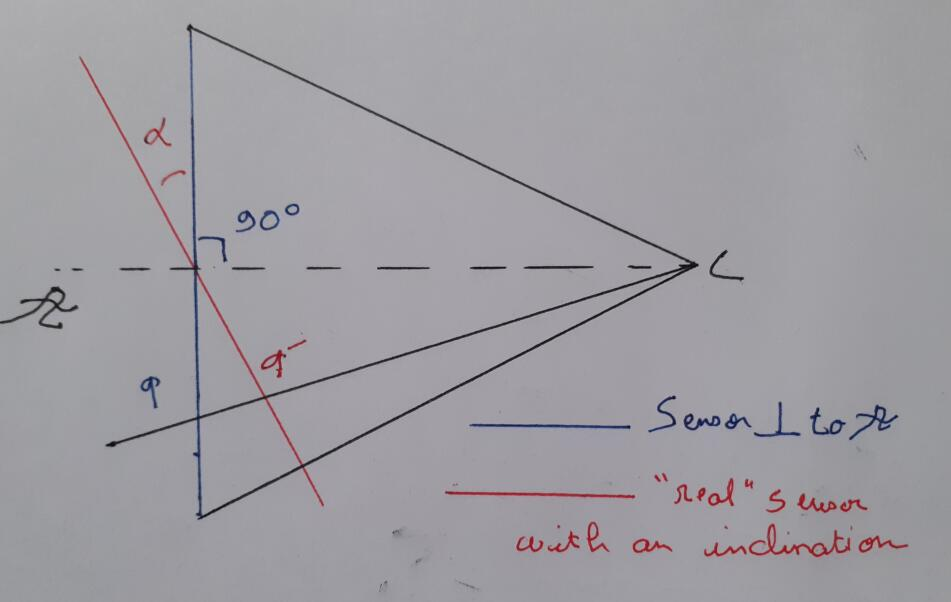
\includegraphics[width=12cm]{Methods/Images/PlanIncl.jpg}\caption{Notation for sensor inclination}
	\label{fig:PlaneIncl}
\end{figure}

The secons hypothesis  that will be questionned is the fact that the sensor is 
orthogonal to axes $\mathcal{A}$.  Using the notation illustatred by 
figure \ref{fig:PlaneIncl}, we will proceed this way :

\begin{itemize}
    \item consider a "theoricall" camera with a sensor orthognal to $\mathcal{A}$ (blue on figure \ref{fig:PlaneIncl});

    \item consider a "real" camera with a sensor tilted (in red);

    \item with consider that rotation is done arround $P^p$, because any global translation of the sensor
         would lead to variation of focal that are already modelized;

    \item  for a given ray, let $q$  be the point that intersect the  orthogonal plane,
	    and $q'$ the point that intersect the tilded  plane, we note
           $\mathcal{T}$  the mapping $\mathcal{T} : q \rightarrow q'$.

\end{itemize}

We will assume that the distorsion $D^t$ of the tilted camera is the combination
of the distorsion of untilted camera and $\mathcal{T}$ :

\begin{equation}
	D^t = \mathcal{T} \circ D 
\end{equation}

%-----------------------------------------------------

\subsection{mathematicall modelisation}

For now we make the hypothesis that the tilt is made by a rotation of angle $\alpha$ arround axe $(O\vec{i})$.
Let $\mathcal{P}_\alpha$ the plane we obtain.  We can compute a basis  of $\mathcal{P}_\alpha$ defines
by  $\vec{i} $ and  $\vec{j}_\alpha $


\begin{equation}
	\vec{j}_\alpha = \begin{pmatrix} 0 \\ \cos(\alpha) \\ \sin(\alpha)  \end{pmatrix}
\end{equation}

To compute the coordinate of $q'$, we use the fact that $q,q',C$ are aligned and $q' \in \mathcal{P}_\alpha$ :

\begin{equation}
        \lambda \begin{pmatrix} x \\ y  \\ 1  \end{pmatrix}
      = x'  \vec{i} + y' \vec{j}_\alpha  + \vec{k}
      =	\begin{pmatrix} x' \\ y'\cos((\alpha)  \\ 1+y'\sin((\alpha)  \end{pmatrix}
\end{equation}


The we compute ratio :

\begin{equation}
	\frac{y'\cos(\alpha)}{1+y'\sin(\alpha)} =  y \;\;\; ; \;\;\;  
	\frac{x'}{y'\cos(\alpha)} =  \frac{x}{y} 
\end{equation}

And solve the equation :

\begin{equation}
	y' = \frac{y}{\cos(\alpha) -y \sin(\alpha)} =  y \;\;\; ; \;\;\;
	x' = \frac{x}{1-y \tan(\alpha)}
\end{equation}



%-----------------------------------------------------
%-----------------------------------------------------
%-----------------------------------------------------

\section{"Universal" model}

\subsection{Assemblage camera}
\subsection{$360$ camera}

\section{Fish eye model}
\label{SecFE}

\section{Note and PPA , PPS and decentric dist}
\label{PPA:PPS:DEC}


\section{Note work to do on non perspective camera}



%-----------------------------------------------------
%-----------------------------------------------------
%-----------------------------------------------------






\chapter{Pose estimation, elementary method}

%-----------------------------------------------------
%-----------------------------------------------------
%-----------------------------------------------------

\section{Introduction}

This chapter present the "elementary" methods, that compute the pose of an image
from observations that can, typically, be tie points (relative pose) or 
ground control point (relative or absolute pose).

By elementary we means algorithms that compute directly a solution for a limited
(typically $2$ or $3$, a few with tomasi-kanade) number of images. These algorithms
are the "tacticle" part, the result of these elementary algorithms will be used as
elementary part of the puzzle by more global method that will try to have a "strategic"  view.


%-----------------------------------------------------
%-----------------------------------------------------
%-----------------------------------------------------

\section{Space resection, calibrated case}

\label{SR_Cal}

    %-----------------------------------------------------
\subsection{Introduction}

We deal here with the following problem,  we have :

\begin{itemize}
   \item a calibrated camera ;
   \item a set of point for which we know the  $3d$ word coordinates $G_k$ and their 
        $2d$ coordinate $p_k$ in a image acquired with this camera;
\end{itemize}


We want to extract the pose $R,C$ of the camera (Rotation,center) such that for every point
we have the usual projection equation:

\begin{equation}
       \mathcal I(\pi (R*(G_k-C))) = p_k \label{EQ:PROJ}
\end{equation}


Each equation~\ref{EQ:PROJ}  creates $2$ constraints : one on line and one on column.
Also the pose $R,C$ has $6$ degrees of freedom, so we can expect that the problem has
a finite number of solution when we have $3$ points (in general less than $3$ will create
infinite number and more than $3$ no solution).

So here we will deal specifically  with the computation of the $R,C$ satisfying
exactly the equation~\ref{EQ:PROJ}  from a set of $3$ correspondance. Other
chapter will discuss of how we use more (possibly many) correspondance for beign 
robust to outlier (for
example with Ransac) or beign more accurate in presence of "gaussian" noise (for 
example with least-square like) .


This problem occurs in two case in photogrammetric pipeline :

\begin{itemize}
   \item the first case is in fact rather rare, it's the case where we have "real" GCP
         an approximate calibration, and want to compute the initial pose of a camera ;
         it's rare because the requirement of having at least $3$ GCP visible is rather
         high; by the way it can occurs in calibrating a camera on a calibration fields
         with many GCP;

 \item the second case is when we have a set of $N$ already oriented camera  ($N\geq 2 $),
       we want to orientate a new camera \emph{relatively} to this set, we have a
       set of $M \geq 3$ multiple tie point , each tie point being visible in the new
       camera and least two of already oriented camera;  when it is the case,
       we can compute for each tie point, by bundle intesection, an estimation of the
       "ground" coodinate of the point in the current system, and then estimate a pose
       for the new camera coherent with the existing one;
       this case is extremely frequent in automatic photogrammetric
       pipeline (at least will be in {\tt MMVII});

\end{itemize}

The {\tt MMVII} code corresponding to this section can be found in 
{\tt PoseEstim/CalibratedSpaceResection.cpp}.

    %-----------------------------------------------------

\subsection{Putting things in equation}

           %  -  -  -  -  -  -  -  -  -  -  -  -  -  -  -
\subsubsection{Equivalence to local coordinates}

\label{SpRes:EquivLocCoord}

First, we remark that if we know the local coordinates $L_k$ of the points in the repair
of the camera, the problem becomes easy . Let show it, we will have to find a translation-rotation such that  :

\begin{equation}
       R*(G_k-C) = L_k  ; k\in{1,2,3} \label{SpResecEQ:WL}
\end{equation}


For each pair $k,k'$, we have (noting $\Vec{X}_{kk'} = \overrightarrow{X_{k}X_{k'}} $):


\begin{equation}
	R* \Vec{G}_{kk'} =  \Vec{L}_{kk'} \label{SpResecEQ:WLVECT}
\end{equation}

As  $R$ is a rotation we have $R(A \wedge  B) = R(A) \wedge   R(B) $ and then:

\begin{equation}
	R* \begin{bmatrix} \Vec{G}_{12} & \Vec{G}_{23} &  \Vec{G}_{12} \wedge \Vec{G}_{23} \end{bmatrix} 
        =  \begin{bmatrix} \Vec{L}_{12} & \Vec{L}_{23} &  \Vec{L}_{12} \wedge \Vec{L}_{23} \end{bmatrix} 
        \label{SpResecEQ:WLVECT}
\end{equation}

Equation~\ref{SpResecEQ:WLVECT} allows to compute $R$ by matrix inversion and multiplication, and 
once $R$ is known it can be injected in equation~\ref{SpResecEQ:WL} to compute $C$.

           %  -  -  -  -  -  -  -  -  -  -  -  -  -  -  -
\subsubsection{Equivalence to compute depth}

We need to compute the local coordinates . For this, we know for each point the bundle its belongs
to because we know internal calibration. Le $B_k$ be the bundle bearing the point $p_k$ We can write symbolicly :


\begin{equation}
	B_k =  \pi^{-1} (\mathcal I ^{-1} (p_k)) \label{SpResecEQ:DefBundle}
\end{equation}



Let write $B_k = (0,\Vec{u}_k)$,  we can compute $\Vec{u}_k$ with internal calibration and
as we know that $L_k \in B_k$ we can write  :


\begin{equation}
	L_k = \lambda_k \Vec{u}_k \label{SpResecEQ:DefLambda}
\end{equation}

So to solve our problem it is sufficent to estimate $\lambda_k$.

           %  -  -  -  -  -  -  -  -  -  -  -  -  -  -  -
\subsubsection{Setting equations}

Now we remember that rotation and translation are isometric, so we have conservation of
distances between  word an local coordinates. We can then write :

\begin{equation}
  D_{kk'}=||\Vec{G}_{kk'}||   = || \Vec{L}_{kk'} || = || \lambda_k \Vec{u}_k -  \lambda_{k'} \Vec{u}_{k'}|| \label{SpResecEQ:ConsDist}
\end{equation}


In equation~\ref{SpResecEQ:ConsDist}, the $D_{kk'}$ and  $\Vec{u}_k$ are knowns, so we have $3$ equation  for
$3$ unkowns, so far so good \dots 



    %-----------------------------------------------------

\subsection{Solving $3$  equations with $3$ unknowns}

\subsubsection{Fix notation an supress 1 unknown}

We change notation to have lighter formula and to make them coherent with the {\tt C++} code of {\tt MMVII}
impplemating this resolution. We call $\Vec{A} , \Vec{B}, \Vec{C}$  the bundles, $D_{AB}$ the distances, \dots
equations become :

\begin{equation}
	D_{AB} = || \lambda_a \Vec{A} -  \lambda_{b} \Vec{B} || \label{SpResecEQ:ABC}
\end{equation}

By doing quotient of equation~\ref{SpResecEQ:ABC} we have :

\begin{equation}
	\rho^A_{bc}  
	=	\frac{D^2_{AB}}{D^2_{AC}} 
	= \frac{|| \Vec{A} -  \frac{\lambda_{b}}{\lambda_{a}} \Vec{B} ||^2 }{||\Vec{A} -  \frac{\lambda_{c}}{\lambda_{a}} \Vec{C}||^2}
	\;\;
	\rho^C_{ba}  
	=	\frac{D^2_{CB}}{D^2_{CA}} 
	= \frac{|| \frac{\lambda_{c}}{\lambda_{a}} \Vec{C} -  \frac{\lambda_{b}}{\lambda_{a}} \Vec{B} ||^2 }
	       {||\Vec{A} -  \frac{\lambda_{c}}{\lambda_{a}} \Vec{C}||^2}
	       \label{SpResecEQ:Lambda}
\end{equation}

Now we see that in equation~\ref{SpResecEQ:Lambda}, only the ratio $\frac{\lambda_{b}}{\lambda_{a}}$ and $\frac{\lambda_{c}}{\lambda_{a}}$
matters, so one can solve them a system of $2$ equation with $2$ unknowns. Once we will have computed these ratio the triangle
$(\Vec{A} , \frac{\lambda_{b}}{\lambda_{a}} \Vec{B},  \frac{\lambda_{c}}{\lambda_{a}} \Vec{C})$ will be propoprtionnal the
triangle $(G_A,G_B,G_C)$ and it will be sufficient to compute this proportion.


           %  -  -  -  -  -  -  -  -  -  -  -  -  -  -  -
\subsubsection{Supression another unknown}

We fix the notation for ratio :

\begin{equation}
	\frac{\lambda_{b}}{\lambda_{a}} = 1+ b  \;\;
	\frac{\lambda_{c}}{\lambda_{a}} = 1+ c
\end{equation}


The $1$ in $1+b$, is to be coherent with {\tt C++} implementation where this make a more numerically stable system.
Also to be coherent with {\tt C++} implementation, we will make the hypothesis that bundles have been normalized :

\begin{equation}
	|| \Vec{A}|| = || \Vec{B}|| = || \Vec{C}|| = 1
\end{equation}

So equations~\ref{SpResecEQ:ABC} rewrites :

\begin{equation}
	\rho^A_{bc}  
	= \frac{|| \Vec{A} -  (1+b) \Vec{B} ||^2 }{||\Vec{A} - (1+c) \Vec{C}||^2}
	= \frac{|| \overrightarrow{AB} +  b \Vec{B} ||^2 }{||\overrightarrow{AC}  + c \Vec{C}||^2}  \label{SpResecEQ:EqFracABC}
\end{equation}
\begin{equation}
	\rho^C_{ba}  
	= \frac{|| (1+c) \Vec{C} -  (1+b) \Vec{B} ||^2 } {||\Vec{A} -  (1+c) \Vec{C}||^2}
	= \frac{|| \overrightarrow{BC} + c \Vec{C} -  b \Vec{B} ||^2 } {||\overrightarrow{AC}  + c \Vec{C}||^2}
	 \label{SpResecEQ:EqFracCBA}
\end{equation}

Now we can write equation~\ref{SpResecEQ:EqFracABC} :

\begin{equation}
	b^2 + 2 b \overrightarrow{AB}. \Vec{B} + (||AB||^2 -   \rho^A_{bc} ||\overrightarrow{AC}  + c \Vec{C}||^2)
	\label{SpResecEQ:Pol2B}
\end{equation}

Equation~\ref{SpResecEQ:Pol2B} can be see as $2d$ degree polynom in $b$, and we can express $b$ as function of $c$:

\begin{equation}
	b = -\overrightarrow{AB}. \Vec{B} \pm \sqrt{Q(c)}  = -\overrightarrow{AB}. \Vec{B} + \epsilon \sqrt{Q(c)} 
	 \;\;\;  \epsilon \in \{-1,1\}  \label{SpResecEQ:SolEqD2}
\end{equation}

With $Q(c)$ being a $2$ degree polynom in $c$:
\begin{equation}
	Q(c) = (\overrightarrow{AB}. \Vec{B})^2 -  (||AB||^2 -   \rho^A_{bc} ||\overrightarrow{AC}  + c \Vec{C}||^2)
\end{equation}

           %  -  -  -  -  -  -  -  -  -  -  -  -  -  -  -
\subsubsection{Resolving last unknown}

We can now use equation~\ref{SpResecEQ:SolEqD2} to substituate $b$  in equation~\ref{SpResecEQ:SolEqD2}

\begin{equation}
	\rho^C_{ba}   ||\overrightarrow{AC}  + c \Vec{C}||^2
	= || \overrightarrow{BC} + c \Vec{C} -  (-\overrightarrow{AB}. \Vec{B} + \epsilon \sqrt{Q(c)}) \Vec{B} ||^2 
	\label{SpResecEQ:EqcInit}
\end{equation}

We note $R(c)$ the $2d$ degree polynom in $c$ defined by :

\begin{equation}
   R(c) =   \rho^C_{ba}   ||\overrightarrow{AC}  + c \Vec{C}||^2
        - Q(c)
        - ||\overrightarrow{BC} + c \Vec{C} + (\overrightarrow{AB}. \Vec{B}) \Vec{B} ||^2
\end{equation}

We note $L(c)$ the $1d$ degree polynom in $c$ defined by :

\begin{equation}
	L(c)=   ( \overrightarrow{BC}.\Vec{B} + \overrightarrow{AB}. \Vec{B} +   c \Vec{C}.\Vec{B}  ) 
\end{equation}

Then equation~\ref{SpResecEQ:EqcInit} writes :

\begin{equation}
	R(c) = 2 \epsilon L(c)  \sqrt{Q(c) }   \label{SpResecEQ:RL}
\end{equation}

Squaring equation~\ref{SpResecEQ:RL} we obtain a $4$ degree polynomial equation :

\begin{equation}
	R(c) ^2 - 4 L(c)^2  Q(c) = 0   \label{SpResecEQ:D4}
\end{equation}

We just need to solve equation~\ref{SpResecEQ:D4} to get possible values of $c$, 
then get values of $b$ using~\ref{SpResecEQ:SolEqD2}, 
then get depth $\lambda _k$, then get local coordinates $L_k$ using~\ref{SpResecEQ:DefLambda} 
and~\ref{SpResecEQ:DefBundle}, and finally finally compute the pose $R,C$  going back to~\ref{SpRes:EquivLocCoord}.

%-----------------------------------------------------
%-----------------------------------------------------
%-----------------------------------------------------

\section{Space resection, uncalibrated case}

    %-----------------------------------------------------

\subsection{Introduction}

We deal here with the following problem,  we have :

\begin{itemize}
   \item an \emph{un-calibrated} camera ;
   \item a set of point for which we know the  $3d$ word coordinates $G_k$ and their 
        $2d$ coordinate $p_k$ in a image acquired with this camera;
\end{itemize}


We want to extract \emph{simulatenously} the pose $R,C$ of the camera (Rotation,center)  and the calibration
$\mathcal I$ such that for every point we have the usual projection equation:

\begin{equation}
       \mathcal I(\pi (R*(G_k-C))) = p_k \label{EQ:PROJ}
\end{equation}

Obviously this problem require more informations ~\ref{SR_Cal}, because we want to estimate more parameters.
Also, due to correlation between internal and external parameters, the solution
are frequently not so stable. It usage is far less current than calibrated case,
to our knowledge, the two cases where it appears practically are :


\begin{itemize}
   \item approximate  orientation of old images for wich we have no idea of focal length and/or principal
        point; one advantage of the method, as it reestimates the principal point, is that it can work
        also with croped images (current case for historical images);

   \item for forcing conversion of  non central perspective sensor to a central perspective sensor
        using  artficial $2d-3d$ correspondances; also theoretically not recommanded~\footnote{it's
        always better to use rigourous modelization when we can}, it can unlock situation where one needs to
        use a software that accept only central perspective sensor; this is the case for example
        with satellite images, if one use "small" patches, then the projection  function can be
        approximate by a central perspetive on this "small" patch ~\footnote{In fact, the accuracy of
        the approximation is a difficult question, depend of the size of the patch, of relief, 
        of the exact sensor \dots}.
\end{itemize}

The {\tt MMVII} code corresponding to this section can be found in 
{\tt PoseEstim/UnCalibratedSpaceResection.cpp}.
    %-----------------------------------------------------

\subsection{Hypothesis}

As we want also to estimate the distorsion, we will have to make some hypothesis
and select a model.  We will make the hypothesis that the distorsion is purely linear, so using
our current modelization we will set :

\begin{equation}
	\mathcal{I}  \begin{pmatrix} u \\ v \end{pmatrix}  = P^p + F \begin{pmatrix} u + b_1 + b_2 v \\ v \end{pmatrix} 
\end{equation}

We remind (see \RefFantome) that we use  only $2$ parameters for linear distorsion 
\footnote {from the $4$ possible linear term in a $2 \times 2$ mapping}
 as $1$ is already include in the focal and another is include
because rotation in the plane is redundant with $3D$ rotation. 

This model is selected, not because it will be always appropriate (it will not !) but because
it is the model  for wich we can have direct solution. Sometime we will need less parameters,
for example we "know" that $b_1=b_2=0$ , or we can  know that $P^p$ in the middle of image. Sometime
we will need more parameters, for example adding a radial distorsion. And also sometime
"more and less" \dots When we require other calibration model, we still can use this method to compute
an initial solution and then make a bundle adjustement to refine the model.

    %-----------------------------------------------------

\subsection{Setting equations}

We write $A \sim B$ the relation indicating that $A$ and $B$ are colinear :

\begin{equation}
	  A \sim B   \Leftrightarrow  \exists \lambda : A =  \lambda B
\end{equation}

This projective relation, is related to image formula via :

\begin{equation}
	 \begin{pmatrix} u \\ v \end{pmatrix}  = \pi_0  \begin{pmatrix} x \\ y \\z  \end{pmatrix}
   \Leftrightarrow   \begin{pmatrix} u \\ v \\ 1 \end{pmatrix}  \sim  \begin{pmatrix} x \\ y \\z  \end{pmatrix}
\end{equation}

We have, noting $\mathcal{C}_{al}$ the calibration matrix :

\begin{equation}
	   \begin{pmatrix} i \\ j \\ 1\end{pmatrix}
      =   \begin{pmatrix} P^p_x + F(u+p_1u+p_2v) \\ P^p_y + F v \\ 1\end{pmatrix}
      =  \begin{pmatrix} F(1+p_1) & F p_2 & P^p_x ) \\  0 &   F & P^p_y \\  0 & 0 &1\end{pmatrix} * \begin{pmatrix} u \\  v \\ 1\end{pmatrix} 
	      =  \mathcal{C}_{al} \begin{pmatrix} u \\  v \\ 1\end{pmatrix} 
              \label{UCResecCalibM}
\end{equation}

We have also :

\begin{equation}
	 \begin{pmatrix} u \\  v \\ 1\end{pmatrix}
		 \sim P_c =  \trans R(P-C)
\end{equation}

So :
\begin{equation}
	   \begin{pmatrix} i \\ j \\ 1\end{pmatrix}
		   \sim \mathcal{C}_{al}  \trans R  (P-C)
\end{equation}

Noting $  \mathcal{M} =  \mathcal{C}_{al}  \trans R $, and $Tr = -\mathcal{M} C$, we have :

\begin{equation}
	\begin{pmatrix} i \\ j \end{pmatrix} = \pi_0 ( \mathcal{M} P + Tr )
\end{equation}

Noting :

\begin{equation}
	\mathcal{M}   =  \begin{pmatrix} a & b & c \\ d & e & f \\ g & h & i \end{pmatrix} 
   \;\;\; ; \;\;\;
	 Tr  =  \begin{pmatrix} t_x \\ t_y \\ t_z \end{pmatrix} 
\end{equation}

We finaly have :

\begin{equation}
	i = \frac{ax+by+cz+t_x}{gx+hy+iz+t_z}
   \;\;\; ; \;\;\;
	j = \frac{dx+ey+fz+t_y}{gx+hy+iz+t_z}
	\label{EqHomSRU}
\end{equation}

    %-----------------------------------------------------

\subsection{Solving equation}

    %-----------------------------------------------------
\subsubsection{General approach}

We want to compute $\mathcal{C}_{al},R,C$  from a set of correspondance $(i,j) (x,y,z)$.
We will proceed in $2$ steps :

\begin{itemize}
     \item estimate $a,b\dots ,t_x \dots$, i.e. $\mathcal{M}$ and $Tr$ using equation \ref{EqHomSRU};
     \item extract  $\mathcal{C}_{al},R,C$ from $\mathcal{M}$ and $Tr$;
\end{itemize}


    %-----------------------------------------------------
\subsubsection{Homography estimation}

Equation~\ref{EqHomSRU} is a classical equation for computing unknown homography.
Considering that $i,j,x,y,z$ are observations and $a,b\dots ,t_x \dots$ are unknowns, we can write it 
as :

\begin{equation}
	0 = {ax+by+cz+t_x} -i (gx+hy+iz+t_z)
   \;\;\; ; \;\;\;
	0 = dx+ey+fz+t_y - j (gx+hy+iz+t_z)
	\label{EqLineSRU}
\end{equation}

The nice point is that equation~\ref{EqLineSRU} is linear, easy to solve and with
many observations, we can use least square approach. The bad point is that,
as there is no constant occuring in it: 

\begin{itemize}
    \item the system is ambiguous , if $S$ is a solution $\lambda S$ is a solution
    \item worst, the null vector is a perfect solution that will always annulate the residual
	    of the least-square system.
\end{itemize}

There is different way to overcome this problem. We indicate the way used in {\tt MMVII}.
The trick, as equations ~\ref{EqLineSRU} are defined up to a scaling factor is to fix the
ambiguity by fixing arbitrary one of the variable to a non null value, for example $a=1$ or $t_z=1$. 
But which of the variable must we fix ?  If we make a bad choice, will it have an influence on the
quality.  The method we use is in fact to not really make a choice! We test all the
possible variable, each test lead to a solution and we use equation~\ref{EqHomSRU} to
select the best solution. Note, that it is fast, as the normal matrix is computed only once.
For more detail on the implementation please refer to the code which is densely
documented.


    %-----------------------------------------------------
\subsubsection{Un-mixing parameters}

Sometime, it will be sufficient to know $\mathcal{M}$ and $Tr$, because
with them we can project any point in the image using equation~\ref{EqHomSRU}.
But in other case, we will need to recover the "physical" parameters.

Considering the center, it is easy to compute it, from $Tr = -\mathcal{M} C$, we have :

\begin{equation}
     C= - \mathcal{M}^{-1} Tr
\end{equation}

Computing $\mathcal{C}_{al}$ and $R$ from $\mathcal{M}$, is a classical problem
from matrix algebra, we want the decomposition :

\begin{itemize}
    \item   $\mathcal{M} = \mathcal{C}_{al} \trans R $
    \item   $\mathcal{C}_{al} $  is a triangulas superior matrix;
    \item   $R $  is a rotation matrix;
\end{itemize}

The decomposition of $\mathcal{M}$ is almost what is known to
be the $QR$ decomposition, where $Q$ is orthogonal and $R$ triangular superior
\footnote{we use this  denomination, as it is universal, be aware that it is
error prone as $R$ is not the rotation !}
The eigen library, and most current matrix library offer efficient implementaion
of $QR$ decomposition as it is one of the central method for solving linear
equation \footnote{solving a linear system becomes trivial if matrix are
triangular or othogonal}
So $QR$ decomposition almost save our problem \dots except many details :

\begin{itemize}
    \item what we need is $RQ$ decomposition and not $QR$; by the way it's easy
          by transposition and some column/line symetry to use $QR$ method to make $RQ$,
          interested reader can see the {\tt MMVII} method {\tt RQ\_Decomposition};

    \item $QR$ decomposition is ambiguous up to sign-matrix \footnote{a diagonal
          matrix with only $\pm 1$ on the diagonal}; let $S$ be any sign matrix, we have $SS=Id$,
          then we have $QR=(QS)(SR)$, $QS$ is still orthogonal and $SR$ is still triangular;
          in the {\tt MMVII} library , the $RQ$ decomposition method make a post processing
          to have positive diagonal (it is easy as letf/right multiplying by a sign matrix is only 
          a matter of changing the sign of line/column);
          
    \item let write $\mathcal{M} = T O $ the result of $RQ$ decomposition \footnote{$T$ triangular,
          $O$ orthogonal},  $\mathcal{M} $ is defined up to a scaling factor, so are $T$ and $O$;  this has two
          consequences

          \begin{itemize}
                \item for $\mathcal{C}_{al} $, we see in equation~\ref{UCResecCalibM} that
                     $\mathcal{C}_{al}(2,2)=1$, so  we just have to do
                     $\mathcal{C}_{al}(2,2) = \frac{T}{T(2,2)}$

                \item for $R$, there can be a global sign ambiguity , so we test the determinant of
                      $O$ and do something like $R=\frac{\trans O}{det(O)}$;
          \end{itemize}

\end{itemize}

Recovering all the internal parameters using {\tt MMVII} convention  is now direct :

\begin{itemize}
    \item  $F=\mathcal{C}_{al}(1,1)$ , $P^p_x=\mathcal{C}_{al}(2,0)$,  $P^p_y=\mathcal{C}_{al}(2,1)$;
    \item  $p_1=\frac{\mathcal{C}_{al}(0,0)}{F}-1$ ;
    \item  $p_2=\frac{\mathcal{C}_{al}(1,0)}{F}$ ;
\end{itemize}





% (I)    (PPx + F (u  p1 u + p2 v))     (F(1+p1)   p2F  PPx) (u)     (a b c) (u)      (u) [EqCal]
% (J) ~  (PPy + F v               )  =  (0         F    PPy) (v)  =  (0 e f) (v) =  C (v)
% (1)    (                       1)     (0         0     1)  (1)     (0 0 1) (1)      (1)


%-----------------------------------------------------
%-----------------------------------------------------
%-----------------------------------------------------

\section{Ortographic case with Tomasi-Kanabe}

%-----------------------------------------------------
%-----------------------------------------------------
%-----------------------------------------------------

\section{$2$-images orientation with essentiel matrix}

%-----------------------------------------------------
%-----------------------------------------------------
%-----------------------------------------------------

\section{$2$-images, case planary scenes}


    %-----------------------------------------------------

\subsection{Notes for TD}


\begin{verbatim}
TD1 : SPACE RESECTION

*  Begin with a calibrated camera w/o distortion,
*  From $3$ point compute 2 lamba with MMVII , then generate the rotations, solve ambiquity (with $4$ points)
*  From data with outlier (50\% on 50 point) use ransac like to make a robust init.

*  Do the same thing with distorsion => inverse disorsion (iterative method ? Lesqt Sq ? Majical optimzer of pytthon ?)

*  eventually => interface


TD2 :  CMP CALIB

TD3 : CALIB CONV
\end{verbatim}





\include{Methods/AimeDesc}


\chapter{The "Aime" methods for Tie Points computation}


% Conclusion, on peut sans doute limiter le nombre de point avec ScaleStab
% pour filtrage a priori => genre les 500 les plus stable

%---------------------------------------------
%---------------------------------------------
%---------------------------------------------

\section{Fast recognition}

%---------------------------------------------

\subsection{Motivation}
For each image, we have computed tie points. A tie points is made
of a vector $V \in \RR^n)$ . Typically $V$ is invariant
to the main geometric deformation .  Le  $V_1$ and $V_2$
be two tie points, we note :

\begin{itemize}
   \item  $H_{om}(V_1,V_2) $ the fact that two tie points are homologous;
\end{itemize}

Given $V_1,V_2$, there is of course no no oracle that can indicate if  $H_{om}(V_1,V_2)$,
and classically we want to compute  a fast mathematical function $\Psi $ that indicate if two vector $V_1$ and $V_2$
correspond to the same tie points .  The ideal function would be such :

\begin{itemize}
   \item  $\Psi(V_1,V_2)  \iff H_{om}(V_1,V_2)$
\end{itemize}


Of course this impossible, and we introduce the miss rate  and fall out:

\begin{itemize}
   \item   miss rate , probability of $\Psi=0$ knowing $H_{om}=1$ , we note $p_m$;
   \item   fall out , probability of $\Psi=1$ knowing $H_{om}=0$, we note $p_f$;
\end{itemize}

As we cannot have the ideal function $\Psi $ such as $p_m=0$ and $p_f=0$,
we have to compromise, and depending on the circunstances, the price of the
two error, will not be the same. Typically, in indexation step,  we are especially
interested to have a low $p_f$; converselly in recognition step we are
especially interested to have a low  $p_m$.


\subsection{Bits vector}


\section{Gaussian pyramid}

\subsection{Computing $\sigma_0$}

\label{GP:SIGMA0}

The gaussian pyramid is made from a succession of image at different scale that
result from a gaussian filter. How can we justify it :

\begin {itemize} 
   \item  image $I_k$ must be at resolution  $R_k =  R_0 s ^k$,
   \item if we assimmilat  $I_0$ to a (sum of) gaussian of std dev $\sigma_0$  , $I_k$
         must be (sum of)  gaussian  $\sigma_0 * R_k$ 
   \item so we can write $I_k = I_0 \ast G(\sigma_k)$ with $\sigma_k^2 + \sigma_0^2 = (\sigma_0  R_k)^2$;
\end {itemize} 

To compute the pyramid, we need an estimation of $\sigma_0$. Which is quite natural, if the initial
image is very blured, it a high $R_0$, and the value $R_1-R_0 = (s-1)R_0$ is also high, which require
a high value for gaussian filter.

We need a way to estimate the initial value $\sigma_0$. Also it's quite arbirtrary, the way it is
done in MMVII is :


\begin {itemize} 
   \item  assimilate $I_0$ to a gaussian of  std dev $\sigma_0$;
   \item  suppose $I_0$ is well sampled (nor blurred nor aliased);
   \item we traduce it mathematically by  :
\end {itemize} 

\begin{equation}
    \int_{-\infty}^{+\infty} I_0 |x| = \frac{1}{2}
\end{equation}

Due to symetry , we can replace by integral on $[0,+\infty]$ and supresse absolute value :

\begin{equation}
    \int_{0}^{+\infty} \frac{x}{\sigma_0 \sqrt{2\pi}} e^{-\frac{x^2}{2\sigma_0^2}}  = \frac{1}{4}
\end{equation}

We integrate :

\begin{equation}
      \lbrack  \frac{-\sigma_0}{\sqrt{2\pi}} e^{-\frac{x^2}{2\sigma_0^2}}\rbrack  _{0}^{+\infty}  = \frac{1}{4}
\end{equation}

So :

\begin{equation}
      \sigma_0 = \sqrt{\frac{\pi}{8}} \simeq 0.626
\end{equation}


%----------------------------------------
%  A conserver : equations TIPE Lolo
%-----------------------------------------
\COM{
\begin{equation}
   \delta R = \frac{1}{\sigma} \frac{L}{S} = \frac{1}{\sigma}  \frac{2 \pi a }{ e \; dz} 
\end{equation}

\begin{equation}
   \phi  = \iint \overrightarrow{B} \overrightarrow{dS} 
         = B_M \cos(\omega t) \pi a^2
\end{equation}

\begin{equation}
   e = -\frac{d\phi}{dt}= B_M \omega  \sin(\omega t)  \pi a^2
\end{equation}


\begin{equation}
   d P_J = \frac{e^2}{\delta R}  
         = \frac{ (B_M \omega \pi a^2  \sin(\omega t))^2 \sigma_e dz }{2 \pi a}
\end{equation}


\begin{equation}
   <d P_J> = \frac{B_M^2 \; \omega ^2 \; \pi \; a^3 \; e \; \sigma \; dz}{4}
\end{equation}

\begin{equation}
  <P_J> =  \int_{z=0}^H <d P_J> = \frac{B_M^2 \; \omega ^2  \; \pi \;  a^3  \; e  \; \sigma  \; H}{4}
\end{equation}

\begin{equation}
  dU = \delta ^2 Q_{creee} +  \delta ^2 Q_{recue de l'air}
\end{equation}

\begin{equation}
  C dT = <P_J> dt - g 2\pi aH(T-T_a)
\end{equation}

\begin{equation}
  C = \mu c 2 \pi a e H
\end{equation}


\begin{equation}
  \mu c 2 \pi a e H \frac{dT}{dt} = \frac{B_M \omega^2 \pi a^3 e \sigma H}{4} - g 2 \pi a H (T-T_a)
\end{equation}


\begin{equation}
  \tau  \frac{dT}{dt} + T = T_{\infty}
\end{equation}


\begin{equation}
  \tau  = \frac{\mu  c e}{g}
\end{equation}

\begin{equation}
  T_{\infty} - T_a = \frac{(B_M \omega a)^2 e \sigma}{8g}
\end{equation}
}


%---------------------------------------------
%---------------------------------------------
%---------------------------------------------

\section{Matching by relaxation}

\subsection{Notations}

We have two images $I$ and $J$, and two set of characteristic points
in $I$ and $J$ :

\begin{itemize}
   \item $A_i \in I$ for $i \in [1 \cdots M]$;
   \item $B_j \in J$ for $j \in [1 \cdots N]$;
\end{itemize}

We will note $D_{Im}$ the size of the images, typically the length of the diagonal. It will be useful
when we need to set some geometric thresholds.

For each characteristic point, we have both a vector descriptor and a position in the image.
We note :

\begin{itemize}
   \item $A^v_i , B^v_i$  the vector descriptor,  
         $A^v_i, B^v_j \in \mathbb{R}^K $  were the dimension $K$
         is typically some hundreds; however here we are only interested by the fact  there exist 
         some distance $D^v$ between
         vector such that the lower the distance, the more likely is that points are homologous;
         we note $D^v(A^v_i , B^v_i) = D^v(A_i , B_i) $
   \item  $A^p_i , B^p_i$  the position ("pixels")   in images of $A$ and $B$ , 
         $A^p_i , B^p_i \in \mathbb{R}^2$
\end{itemize}


We suppose that we can convert the distance $D^v$ in the likelihood $L$ expressing  that $A$ and $B$
are homologous. For example we  use a threshold $\sigma_v$ and set :

\begin{equation}
    L(A_i,B_j) =  e^{-\frac{D^v(A_i,B_i)}{\sigma_v}} \label{EQ:LikL}
\end{equation}

The transformation from  $D^v$ to $L$  , or even the computation of $\sigma_v$
admitting of formula like \ref{EQ:LikL}, may be an issue. By the way we will admit from
now that we have the function $ L$ , probably a way to rationalize this fact
would be to "learn" it from statistic of "real" homologous points.


\subsection{Formulation}

We want to compute a matching between $A_i$ and $B_j$ that use both the "radiometric context" informations 
and the "spatial consistency" information :

\begin{itemize}
   \item radiometric context : $A_i , B_j$  are matched if, as much as possible, $L(A_i,B_j)$ is high;
   \item spatial consistency : if $A_i$ and $B_j$ are matched, then for each $A'_i$ and $B'_j$ such that ,
         $A'^p_i$ is close to $A^p_i$ and $B'^p_i$ is close to $B^p_i$ , then the likelihood
         to match $A'_i$ and $B'_j$ is higher (i.e. neighbors of my homologous are homologous of
         my neighbors);
\end{itemize}

The principle of relaxation is to compute a non-unique weighted matching and to use
the two pieces of information to iteratively re-compute new value of the weighting. Generally, at
the beginning, the "brute" information (=radiometric context) has a higher importance, and as we go
further we give more importance to relational information (=spatial consistency).

To formalize the problem we consider that we want to compute simultaneously two functions :


\begin{itemize}
   \item a discrete matching function $\psi$  such that $\psi (A_i)$ is the homologous
         of $A_i$, with possibly $\psi (A_i) = 0$  when no match is found for $A_i$,
         and we set  $L(A_i,0) = L_0$ where $L_0$ is a constant;
   \item a geometric \emph{smooth} function $\phi$ .
\end{itemize}

And the criterion on $\psi$ and $\phi$ are to  maximize global
likelihood $\mathcal L(\psi)$ (\ref{Crit:Psi})  while minimizing the
spatial incoherence $ \mathcal S(\psi,\phi)$  (\ref{Crit:PhiPsi}).


\begin{equation}
    \mathcal L(\psi) = \sum  L(A_i,\psi(A_i)) \label{Crit:Psi}
\end{equation}


\begin{equation}
    \mathcal S(\psi,\phi) = \sum  | \psi(A_i)^p - \phi(A^p_i) | \label{Crit:PhiPsi}
\end{equation}

Of course, there must be some strong regularity constraint on $\phi$ so that the
equation ~\ref{Crit:PhiPsi} is not trivial. Generally it belongs to a parametric
space of low dimension (such as similitude, homography ...).


\subsection{Simultaneous $\psi$ and $\phi$ ?}

In most general case, it is quite complicated to compute simultaneously $\psi$
and $\phi$.

\subsubsection{Classical approach}
In the most current case in photogrammetry, a first estimation $\psi_0$ is computed with a simple
strategy as :

\begin{equation}
    \psi_0(A_i) =  \underset{B_j \in J}{\operatorname{argmax}}  L(A_i,B_j) \label{ArgMax:Psi}
\end{equation}

And then $\phi$
is computed to remove false match detected as "outliers" of tested $\phi$. 
There is many tricks to have better result (like symmetric matching), but basically
this is the idea.

A particular and very common case of this simultaneous computation is the case
where $\phi$ represents epipolar geometry and is computed by Ransac. By the way in this
case, the  use of Ransac supposes that we know $\psi$ and that it contains a reasonable
proportion of false matches (typically no more than $50\%$). This case is quite common
for example with images acquired the same time (no diachronism) and tie-points resulting
from SIFT.

\subsubsection{Approach by computing $\phi$ first}

In the problem we want to tackle here, the proportion of false match we would get with
equations like~\ref{ArgMax:Psi} is much too high . So we suppose that we can first
have an \emph{approximate} value $\phi_0$ of $\phi$. We will discuss just after how we can
estimate $\phi_0$.

We have to specify that what we mean by $\phi_0$ is an approximation of $\phi$.
To understand equation~\ref{Phi0:ApproxG}  and~\label{Phi0:Appro} we must
imagine a possible scenario for $\phi$ and $\phi_0$. Typicaly $\phi$, the real
correspondence, will the combination of epipolar geometry and $3D$ scene, so according
to the scene, the $\phi$ can be  continuous or only piece-wise continuous. For $\phi_0$,
in our context it will be a function with few parameters, typically a similitude
plane computed from few points (at least $2$). 

We then formalize "$\phi_0$ approximating  $\phi$" by (see also Fig.~\ref{fig:spatial-consist}) :


\begin{equation}
     | \phi_0(A)  - \phi(A) |  < D_A  \label{Phi0:Appro}
\end{equation}

\begin{equation}
     | (\phi_0(A) - \phi_0(A')) -(\phi(A) - \phi(A')) |  < D_g +  \alpha |A-A'|  \label{Phi0:ApproxG}
\end{equation}

By extension, using equation \ref{Crit:PhiPsi} and criterion $\mathcal S$ we want to minimize,
we will set :

\begin{equation}
     | \phi_0(A)  - \psi(A) |  < D_A  \label{PsiPhi0:Appro}
\end{equation}

\begin{equation}
     | (\phi_0(A) - \phi_0(A')) -(\psi(A) - \psi(A')) |  < D_g +  \alpha |A-A'|  \label{PsiPhi0:ApproxG}
\end{equation}

\begin{figure}
\centering
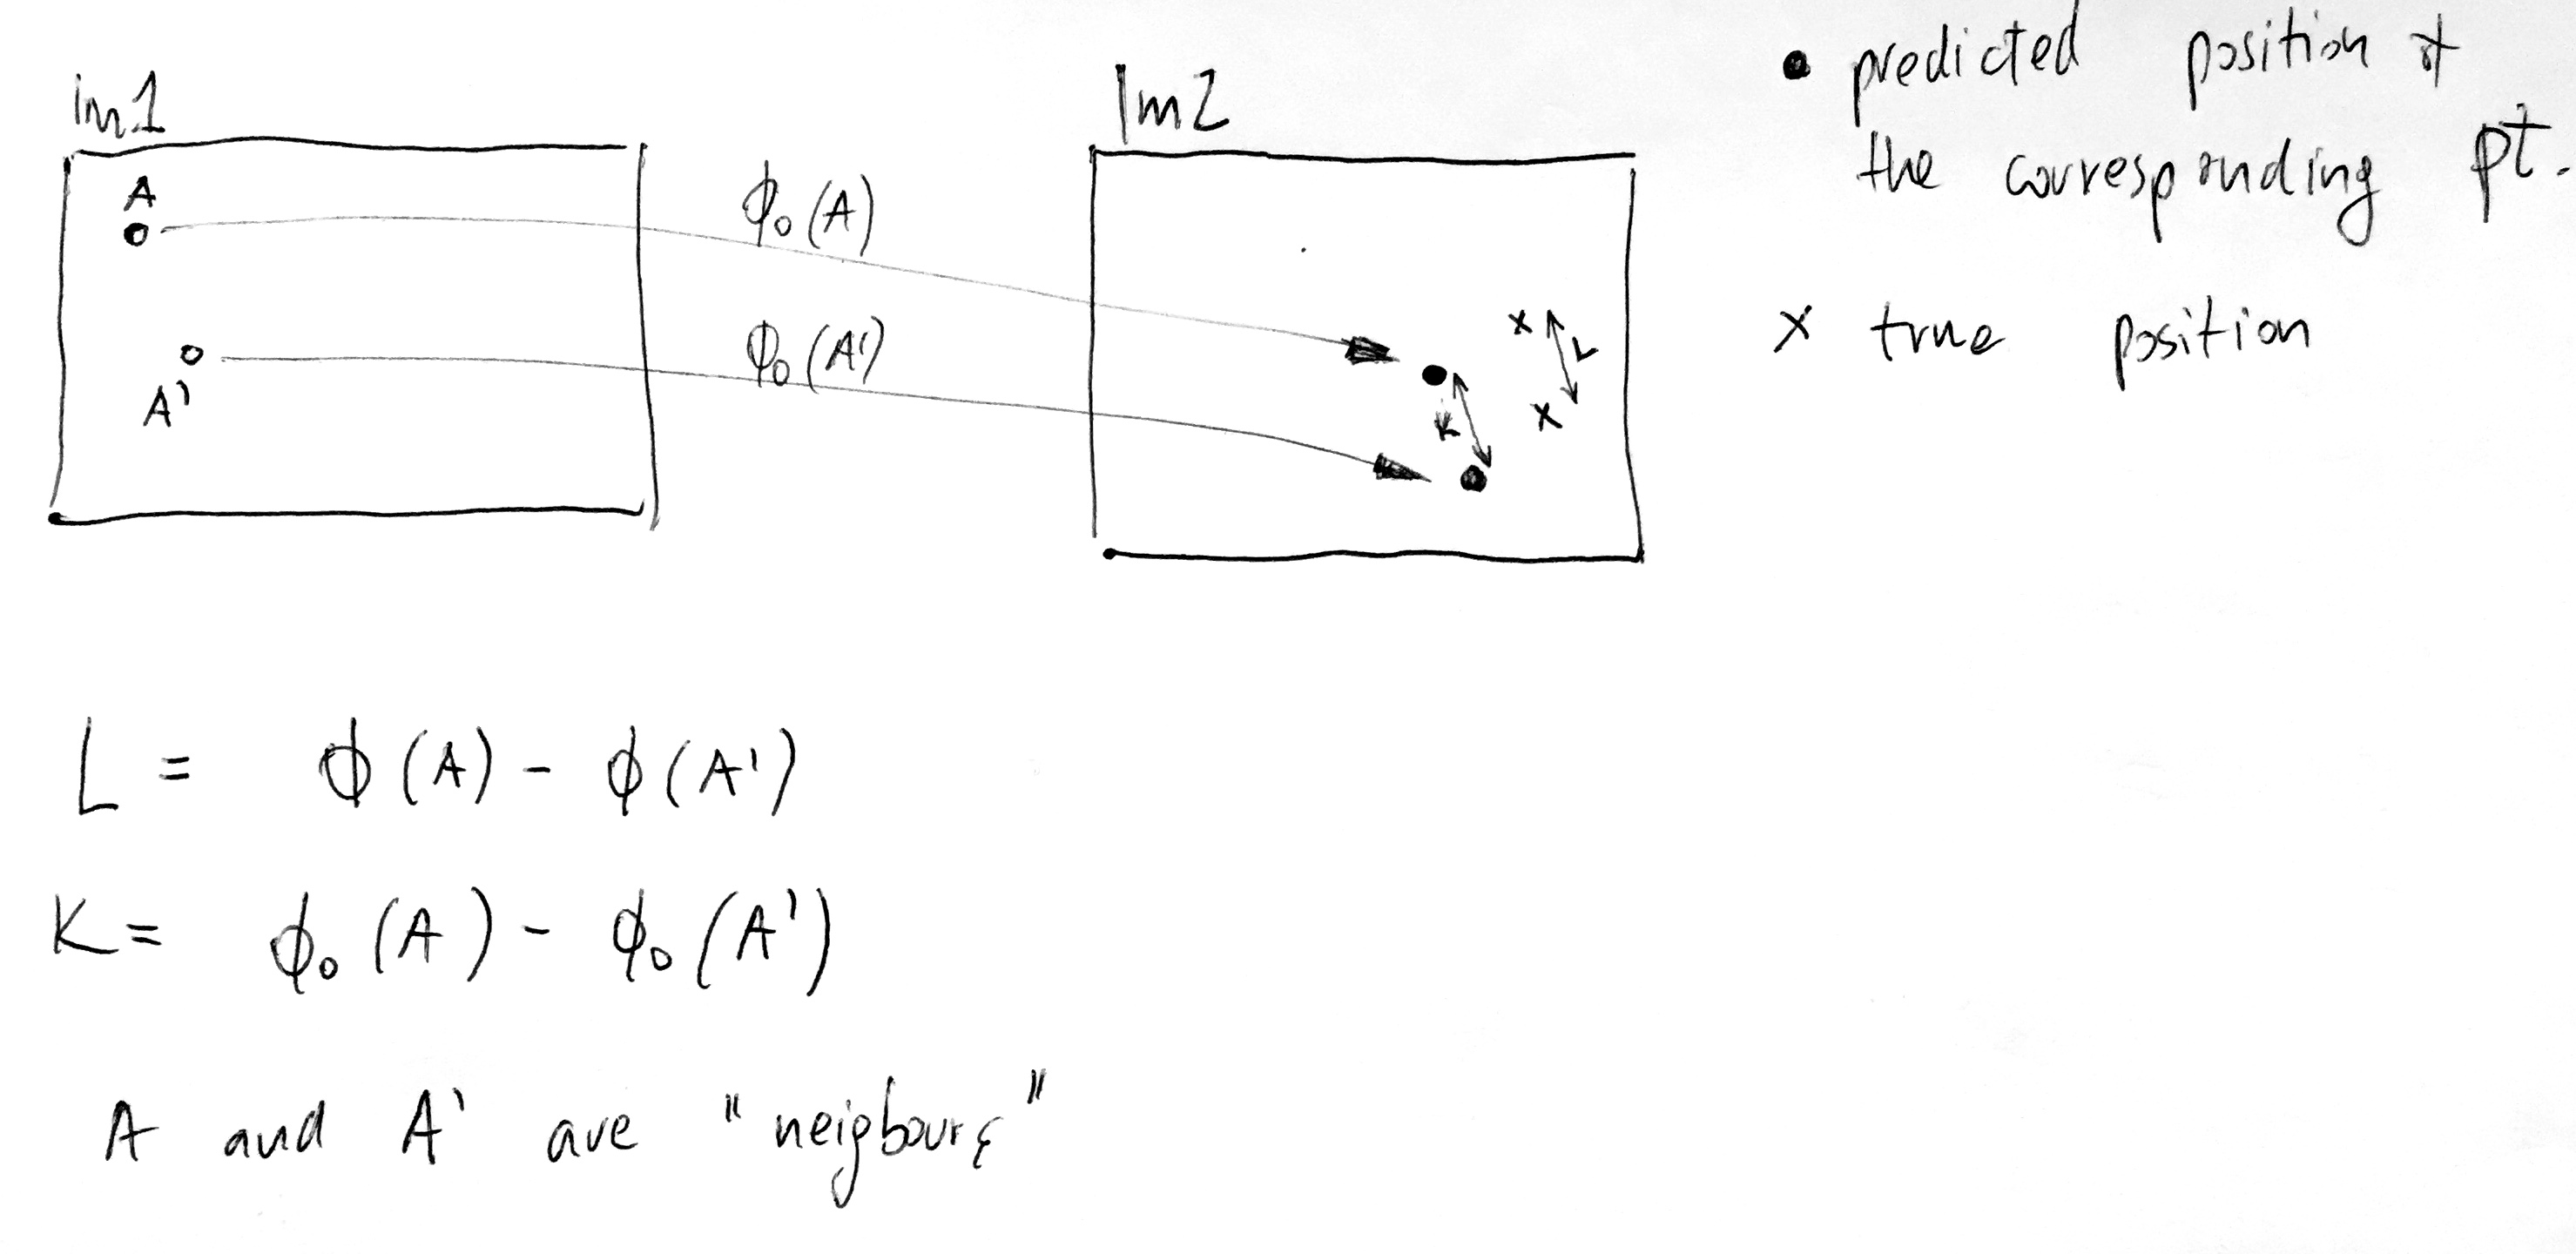
\includegraphics[width=12cm]{Methods/Images/spatial_consist.JPG}\caption{Illustration of equation~\ref{Phi0:ApproxG}.}\label{fig:spatial-consist}
\end{figure}

Let comment these equations  :

\begin{itemize}
   \item in equations~\ref{Phi0:Appro},~\ref{PsiPhi0:Appro},~\ref{PsiPhi0Im:Appro} the value 
         $D_A$ can be relatively high as $\phi0$
         is extracted with few points and the model (similitude) is a rough approximation
         of the "real" model; it seems natural to have $D_A$ proportional to  $D_{Im}$
        (see~\ref{PsiPhi0Im:Appro});

   \item equation~\ref{Phi0:ApproxG},~\ref{PsiPhi0:ApproxG} model the fact that once 
         we "know" that  $ \psi(A)=B$ then $\phi_0$ is a relatively accurate approximation
         of $\psi$ around $A$;  when  $\phi$  is continuous, we don't need $D_g$, however
         when the $3D$ scene is discontinuous, it create discontinuities ; 
         it seems also natural to have $D_g$ proportional to  $D_{Im}$, and obviously
         $D_g$ significantly smaller than $D_A$ (see~\ref{Phi0Im:ApproxG} )
\end{itemize}

So we can write :


\begin{equation}
     | \phi_0(A)  - \psi(A) |  < \beta_A D_{Im}  \label{PsiPhi0Im:Appro}
\end{equation}

\begin{equation}
     | (\phi_0(A) - \phi_0(A')) -(\psi(A) - \psi(A')) |  < \beta_g D_{Im} +  \alpha |A-A'|  \label{Phi0Im:ApproxG}
\end{equation}

Of course, practically, an important question is the values of thresholds $\beta_A, \beta_g, \alpha $.
As a rule of thumb, values of these parameter can be fixed in the following interval :

\begin{itemize}
   \item  $\beta_A \in [0.05,0.2]$, less than $0.05$ would be very optimistic , and by the way this low
          value is probably already sufficient for basic approach like in~\ref{Basic:ArgMax};
          more than $0.2$ would be very pessimistic and by the way difficult to use;

   \item  similarly $\beta_g \in [0.01,0.05]$ and $\alpha \in [0.05,0.3]$
\end{itemize}


And in a first try I woud use $\beta_A=0.1 \;  \beta_g=0.025 \; \alpha=0.15$.


\subsection{Estimation of $\phi_0$}

Obviously, if we cannot estimate $\phi_0$, the previous stuff is useless.
Basically, we can imagine $3$ way to estimate $\phi_0$ :

\begin{itemize}
   \item  the most trivial way is to have an "external" estimation, this can come from
          meta data ("tableau d'assemblage") or from operator measurements (operator select
          manualy two real homologous point and it is sufficient to estimate a similitude);

   \item  another easy way is to use tradional Ransac on a solution like ~\ref{ArgMax:Psi}; 
          with D2Net executed at full resolution, it will probably not work as the proportion
          of false match can be very high; however it is possible to run D2Net at a very low
          resolution, where~\ref{ArgMax:Psi} works not so bad, the accuracy is not so good, but
          it is probably not a problem;

   \item  a third, more sophisticated way, consist to use a non-unique matching at high
          or medium resolution; it is described bellow .
\end{itemize}

Non-unique matching :
\begin{itemize}
   \item  for each point in one image select a number $p$ of its potential matches in the other images, in other words for each point in  $A_i$, select 
            $\Psi (A_i) $ which contains the  $B_j$ corresponding to the $p$
          best scores of $L(A_i,B_j)$; to compute $\Psi$ it is also possible to compute more globally the
          $p * M$ best pairs of all matches $(A_i,B_j)$ where $M$ is a predefined value; here, however, there might be a case where certain points are not assigned a match; to assure that all points have matches a mix of
          both approaches can be adopted (computing a global set of pairs, and also assure to have a minimal
          number of matches per point);

   \item generate solutions, by random selection, if we decide to use similitude,
         it is sufficient to use $2$ pairs of $(A_i,B_j)$  ;  it is also possible to make a biased
         random selection that favors the set of pair having higher likelihood
         (a way to do that is, for each iteration, to generate a few random pairs, 
          and finally select the the pair corresponding to the best likelihood);

   \item for each $2$ pairs, we compute a similitude $S$  and estimate it cost $C(S)$
         by formula below;

   \item after many iteration, select finaly the $S$ minizing $C(S)$.
         by formula above;

\end{itemize}

\begin{equation}
     C(S) = \sum_i (\underset{B_j \in \Psi(A_i)}{\operatorname{Min}}  c(A_i,B_j,S))
\end{equation}

For $c(A_i,B_j,S)$, different formula can be tested, a basic formula proportional to distances, 
one using a threshold to limit the influence of outliers  : 

\begin{equation}
      c(A_i,B_j,S) = Min(|S(A_i)-B_j|,D_A)
\end{equation}

Or a smoother version :

\begin{equation}
      c(A_i,B_j,S) = \frac{|S(A_i)-B_j|}{|S(A_i)-B_j|+D_A)}
\end{equation}

It is also possible to use the likelihood $L(A_i,B_j)$ and merge it with the geometric term , 
however it is always complicated to mix valures of different kind.


\subsection{Basic usage of $\phi_0$}

The easiest way to use $\phi_0$ is to re-use the basic strategy of 
equation~\ref{ArgMax:Psi} but filtering the result with  equation~\ref{Phi0:Appro}  :


\begin{equation}
   \psi_1(A_i) =  \underset{B_j \in \mathcal D(\phi_0(A_i),D_A)}{\operatorname{argmax}}  L(A_i,B_j) 
\end{equation}

Where  $\mathcal D(\phi_0(A_i),D_A)$ is  the disc of center $\phi_0(A_i)$ and radius $D_A$.

\label{Basic:ArgMax}

\subsection{Relaxation}








\chapter{Several stuff unfinished}


%---------------------------------------------
%---------------------------------------------
%---------------------------------------------

%\section{Co-variance propagation}

%---------------------------------------------
%---------------------------------------------
%---------------------------------------------

\section{Bloc fusion}

Hypothesis :

\begin{itemize}
    \item Two bloc $B_1$ and $B_2$  (the method should work with $N$ blocs),
          each has been oriented and we have an unknown similitude to compute between $B_1$ and $B_2$

    \item $N\geq 2$ triangle between $B_1$ and $B_2$
\end{itemize}

We suppose that the rotation has already been solved, which is "easy" because for each triangle,
the $2$ edges between the two different blocs give an estimation.  For each triangle we have an estimation
and quality check ($3$ measures of rotation when $1$ is enough). 

We need to estimate the scale $\Lambda$ and translation $T$. 
Let $P^1$  be a point measured in $B_1$ and $P^2$ be the same point in $B_2$, 
we thus have :

\begin{equation}
	P_2 = \Lambda P_1 + T \label{Eq:Bloc12}
\end{equation}

For each triangle we compute the rotation going to $B_1$ and $B_2$, and we still
have an unknown scale and translation for aligning it on $B_2$.
Let $\lambda_i$ and $t_i$  be the unknown scale and offset of the triangle.
Name $a,b,c$ the three points of a triangle, and $P^a_2, P^b_2 $ their corresponding positions
in $B_2$, which leads to:

\begin{equation}
	P^a_2    = a \lambda_i + t_i     \label{Eq:Bloc:Tri2}
\end{equation}

Now we have two possibilities for each point, if it belongs to bloc $B_2$ we know $P^x_2$ from equation
\ref{Eq:Bloc:Tri2} and we can use it directly. Else, we combine~\ref{Eq:Bloc12} and~\ref{Eq:Bloc:Tri2}
to obtain:

\begin{equation}
	 \Lambda P^a_1 + T = a \lambda_i + t_i \label{Eq:Bloc:Tri1}
\end{equation}

Finally, for  $n$ triangles we solve a \emph{linear} system with $4\cdot(n+1)$ unknowns:
$(\Lambda,T,\lambda_i,t_i)$ and we have $9\cdot n$ equations (by the way, even if we have 
$9$ equation for $8$ unknowns, the system is unslovable for $n=1$, explain why).

Proposed method :

\begin{itemize}
    \item if there are two triangles use ~\ref{Eq:Bloc:Tri2} and ~\ref{Eq:Bloc:Tri1}
          to estimate $\Lambda,T$;

    \item if there are $N>2$ triangles use some ransac strategy by selecting a pair of triangles
          and use previous case to solve it;

     \item if there is $1$ triangle, give up for now;  maybe later, use homologous point between
	     blocs, and outside the triangle to fixe the scale ????

\end{itemize}










\part{Programmer's doc}

% -------------------
% -------------------
% -------------------

\chapter{Programming organisation, style ...}

\section{Naming convention}

\section{Never use {\tt std::cout, printf \dots}}

\section{Encapsulation of boost, stl ..}
\section{Error handling}

%------------------------------------------------------------------
%------------------------------------------------------------------
%------------------------------------------------------------------

\section{Memory check}


%------------------------------------------------------------------
\subsection{Detecting memory leak}

Once memory leak has been detected, if the programmer cannot find easily the source of
this leak, \PPP offer the following facility :

First \PPP must be at its highest level of debug in file {\tt MMVII\_Error.h} :

\begin{verbatim}
#define The_MMVII_DebugLevel The_MMVII_DebugLevel_InternalError_micro
\end{verbatim}

Then compile and run a first time  the command that generate the leak, the identifiant of first
object having generated the link will appears on the console :

\begin{verbatim}
========================== Ident of Non Freed object  102
\end{verbatim}

Now run again the same command using option the option {\tt NTOC4ML} under the debugger, the programm
will stop the execution at the creation of the object, the debugger allowing to inspect the context ,
will get something like that:

\begin{verbatim}
gdb MMVII
...
 run   .... NTOC4ML=102
 ....
 Mes=[Creation of object tagged for memory leak tracking]
 ....
.... in MMVII::cMemCountable::cMemCountable...
...  MMVII::cMemCheck::cMemCheck (this=0x555557d54d58) ....
...  MMVII::cDataGenUnTypedIm<2>::cDataGenUnTypedIm ....
....
...  MMVII::cAppliCheckBoardTargetExtract::DoOneImage  ...
...
\end{verbatim}



%------------------------------------------------------------------
%------------------------------------------------------------------
%------------------------------------------------------------------

\section{Serialization}
\section{Shared pointer}

\section{Random number}

\PPP use some pseudo random generator. As every such generator
they must be initialized with a seed.
By default , the seed is always the same to facilitate debuging.
When user wants initialization from time this must be specified 
with a negative value of parameter {\tt  SeedRand}.



\section{Enum to string}

The enum/string  conversion is a recurent problem of \CPP which
as far as I know is still an issue. A possible solution
would be to use some code genration which from easy to read
an write text file woul generate it. But I tried to limitate
the code generation in \PPP.

In file {\tt Serial/uti\_e2string.cpp} is implemanted 
the used solution , it consist  to create data for each enum
for which we want to do the conversion {\tt Serial/uti\_e2string.cpp}.







\chapter{Use of non linear optimization in MMVII}

\label{Chap:NLO}

This chapter is targeted for programmer that will increase MMVII, it mainly describe classes
interfaces in headers and a detailled example of using this classes in a cpp file.
 It's not useful for advanced users; on the other hand, for programmer who will maintain the core of MMVII, 
more detailled documentation will have to be written.

At this step, the chapter has no theoretical presentation, it assumes that the reader is familliar
with least square, linearization, Gauss-Newton, Schur complement\dots


%---------------------------------------------
%---------------------------------------------
%---------------------------------------------

\section{Introduction}

%---------------------------------------------

\subsection{Quick formalization}

This chapter presents the classes used in MMVII for non linear optimisation using some Gauss-Newton methods. 
By non linear optimisation, we mean minimize $F(X)$ with :

\begin{equation}
      F(X) = \sum_{j=1,M} w_j f_j(X)^2  \;  X \in \RR^n  \label{EqNLOInit}
\end{equation}

The assumpution on the problem are classical :

\begin{itemize}
   \item we have an initial guess $X_0$ on $X_{min}$  , this guess is sufficiently 
         good for the local minimal we will (hopefully) find to be a global minimum;

   \item the function $f_j$ are differentiable (some weaker hypothesi are also possible)

\end{itemize}

The service offered by MMVII are typically those a Gauss-Newton iterations : 
use current estimation $\tilde X$ of $X_{min}$ for linearizing the $f_j$ and 
solve equation $\ref{EqNLOInit}$ by least square methods.

%---------------------------------------------

\subsection{2d-Triangularton problem in general}

We will illustrate the presentation by a detailled example that is used for testing correctness of the
implementation. Also relatively basic, this example should be sufficient for a first 
understanding and utilisation of the MMVII classes. The $2d$-triangulation problem we treat
here is the following :

\begin{itemize}
    \item we have a set of points $P_1 \dots P_n$ , each $P_k$ belongs to $\RR^2$;

    \item we do not know the exact values of $P_k$ but we have an initial estimation  $P^0_k$
          which is not too bad, whatever it means;

    \item for a certain number of pair $P_i,P_j$ we have a measurement of the distance $d_{ij}$ between
          $P_i$ and $P_j$,
\end{itemize}

The triangulation problem  consist to use the measurement of distances for recovering the unknown
value on $P_i$.  Let $M$ be the  number of pair for which we have measurement 
Let $X \in \RR^{2n} = \{P_1 \dots P_n\}$ be the unkown vector,
we typically want to find $X$ that minmize $D$ defined by :

\begin{equation}
      D(X) = \sum_{j=1,M} (d_{ij} -d(P_i-P_j))^2  \label{EqConsDist}
\end{equation}


Of course as the fonction $D$ is invariant to any isometry of the plane, the minimization
of $D$ would be an ill-posed problem, as for any set of points, its image by a global rotation
will give the same value. To ensure uniqueness of the solution  will force the value of
a certain number of coordinates.

%---------------------------------------------

\subsection{2d-Triangularion in this example}

As we want the example to be as simple as possible, and also we want to use it for checking
the correctness, the data will be different from a real one , the figure~\ref{fig:NetFull} illustrates 
this network:

\begin{itemize}
    \item the "real" value of points will be positionned on a regular grid, typically we
           will have $(2*N+1)^2$ points, each point having integers corrdinate 
           $(x,y) \in [-N,N]^2$

    \item we will have measure between pair of point that  are $8$-neighoor i.e
          $max(|x-x'|,|y-y'|)\leq 1 $ , this is sufficient for the solution to be unique
          up a rotation ;

    \item in real life  $d_{ij}$ would be noisy, but here in this simulation example we
          use the exact value because, to check correctness of the library, we want to check 
          that we are able to recover the exact values of coordinates.
\end{itemize}

Regarding the arbirtrary constraint we will keep it as simple as possible, so 
considering the two points of the grid  $A=(0,0)$ and $B=(0,1)$ , we will add the following
constraint to the minimization :

\begin{equation}
      x_A=0  \;  y_A=0  \;  x_B=0 \label{Eq:FixVarAB}
\end{equation}

The two first constraint freeze the solution in translation, while the last one freeze the rotation.


\begin{figure}
\centering
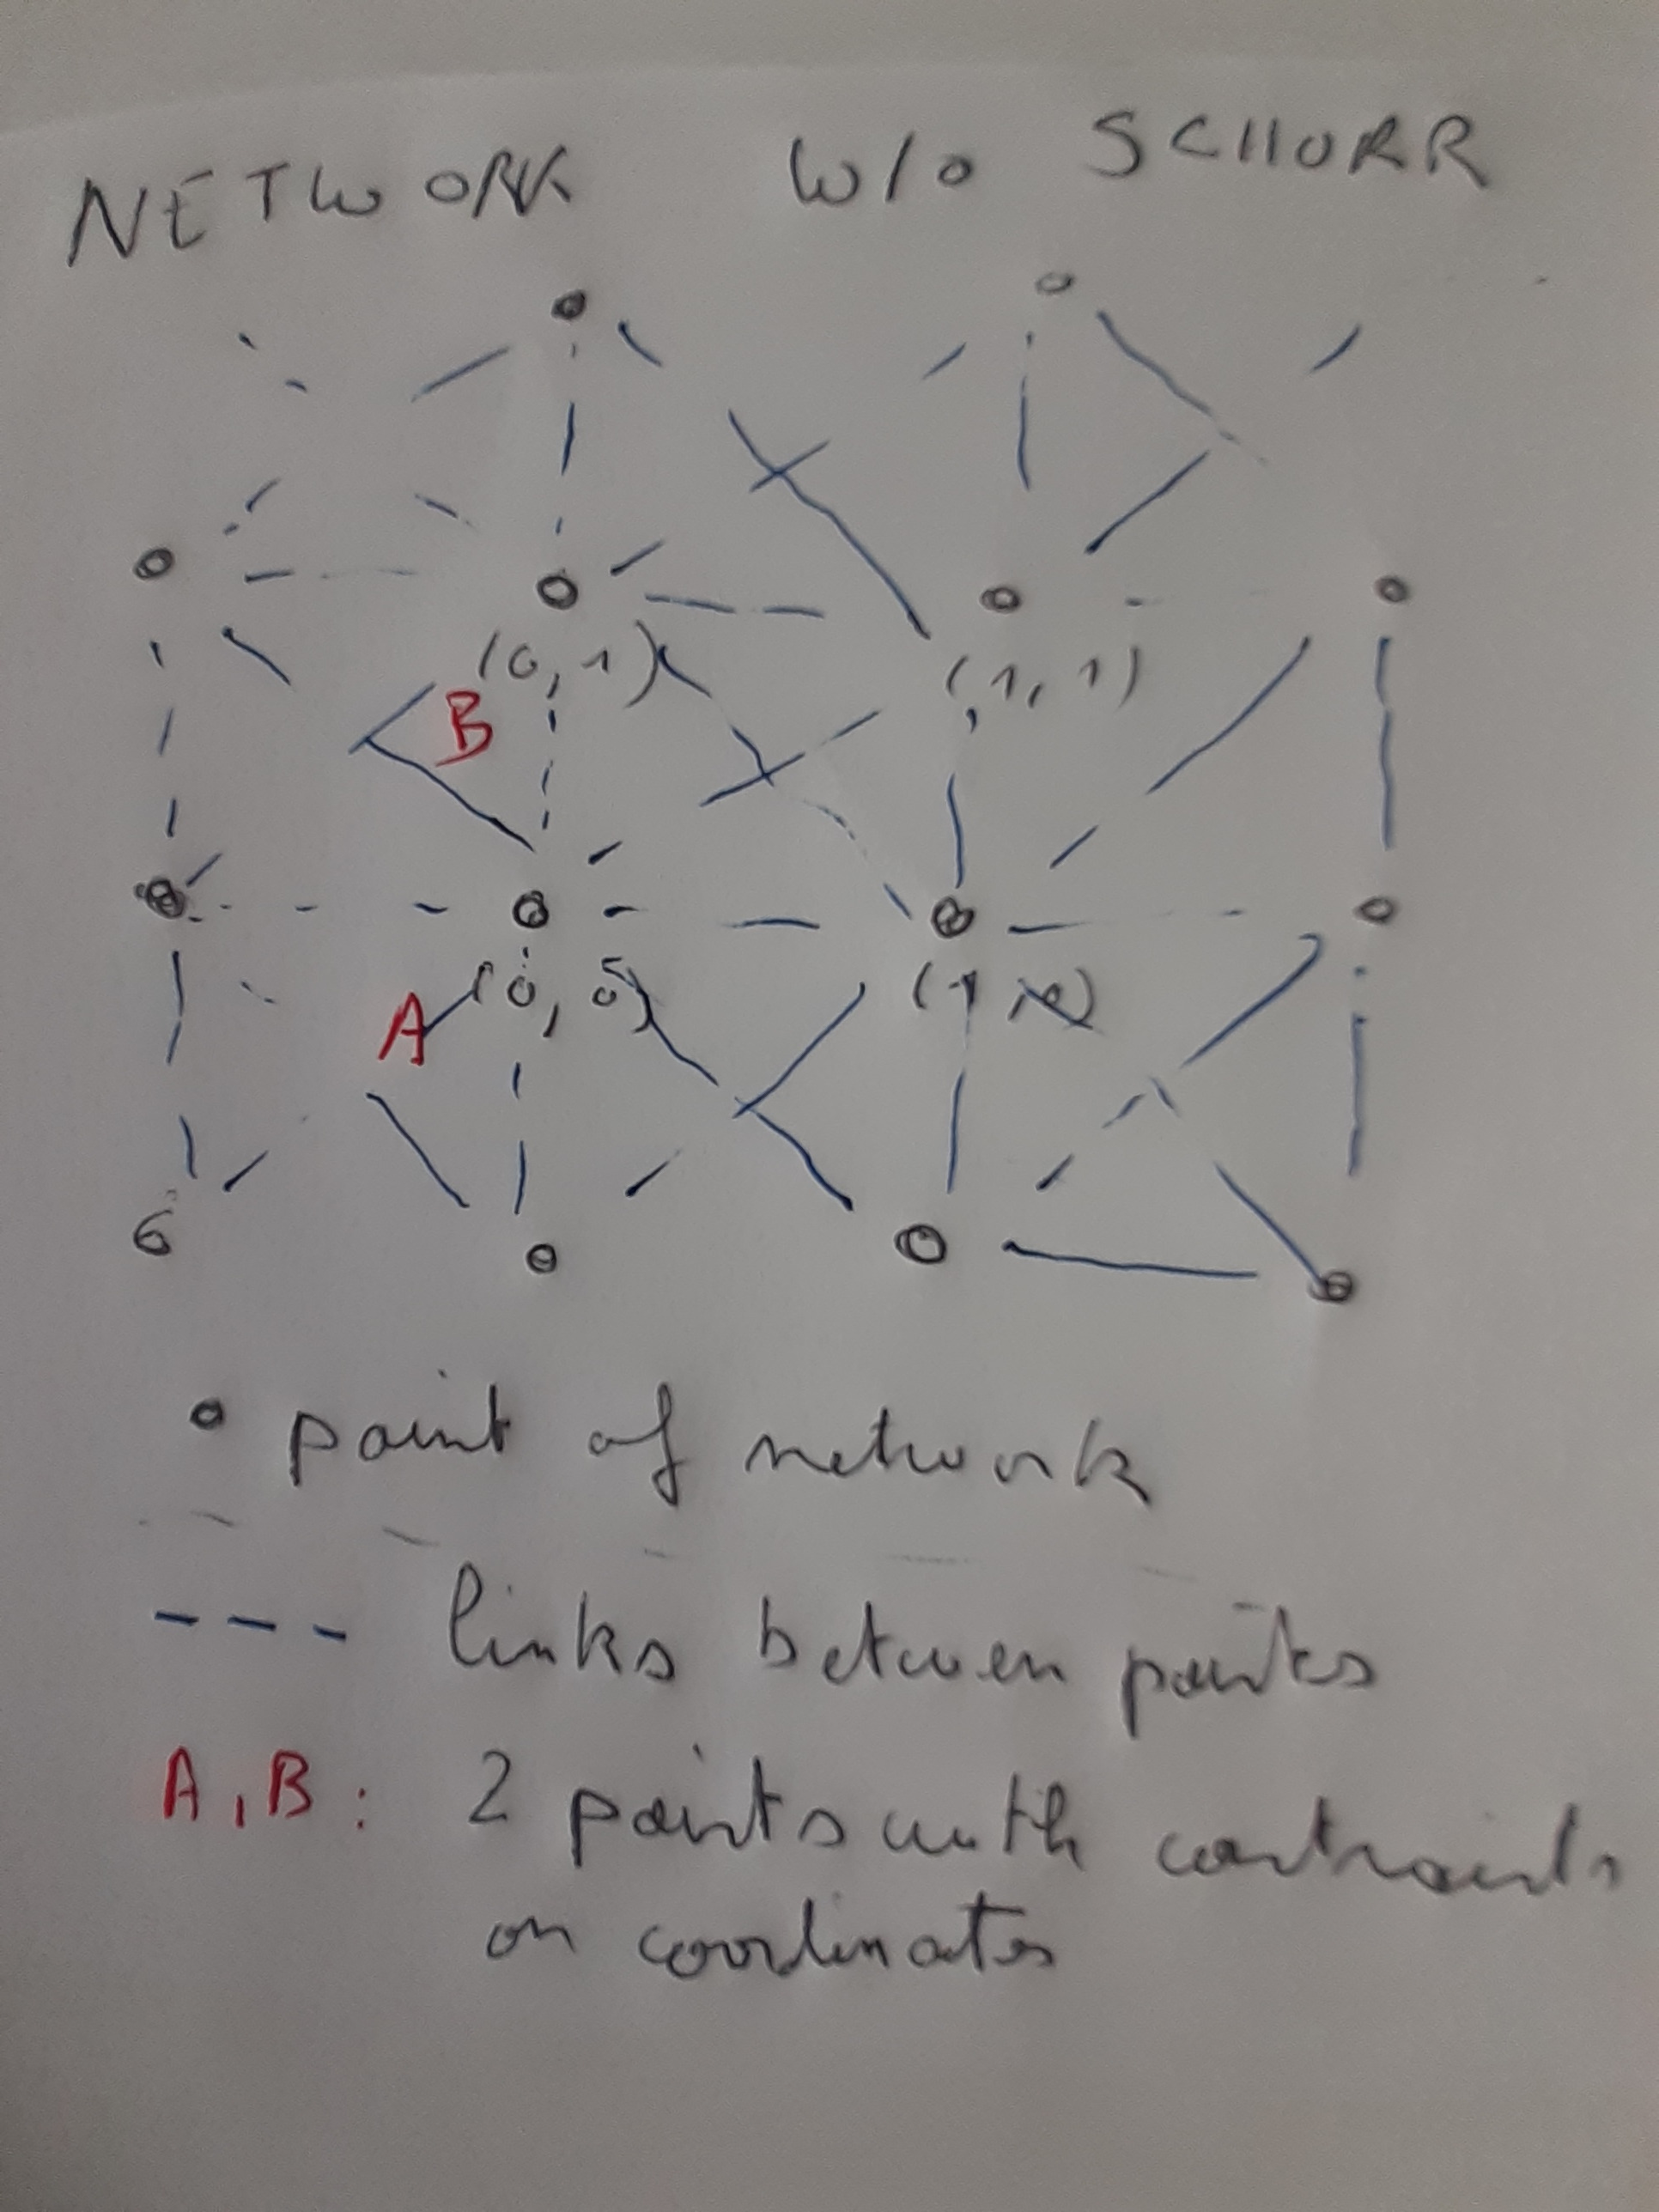
\includegraphics[width=12cm]{Methods/Images/T90-NetFull.JPG}\caption{Network, case w/o schur}\label{fig:NetFull}
\end{figure}



%---------------------------------------------

\subsection{Use of schur complement}

Schur complement is an efficient way to treat the case where there is a subset of variable that 
occurs in \ref{EqNLOInit}, but for which we are not specially interested in exact values ,
 however but we want to take them into account rigourously in 
the computation of the others. Once we know
\emph{all} the equations where such  subset of variable is involved, schur
complement offer a way to eliminate them without altering the value of the minimum.

A typical case is in bundle adjsutment, when we are interested only to the value
of camera parameters and not by the value of $3d$ points involved by the projection
equation. In this case, suppose we will typically  have $1000$ camera and $1000000$ points,
doing schur elimination can reduce the system from $3000000$ unkwnon to $6000$.



In our toy example, the schur complement will be purely artificial. When the
{\tt WithSchur}  option is activated, the network is modified in the following
way, the figure~\ref{fig:NetSchur} illustrates 

\begin{itemize}
    \item all the points on the line $x=1$ are considered as temporay variable,
          i.e variable that we want to eliminate, we will not  know their value at the
          end of the computation; 

    \item there will be no conexion between points of line $x=1$ (for example $(1,2)$
          and $(1,3)$ that were connected in previous case are non longer
\end{itemize}

\begin{figure}
\centering
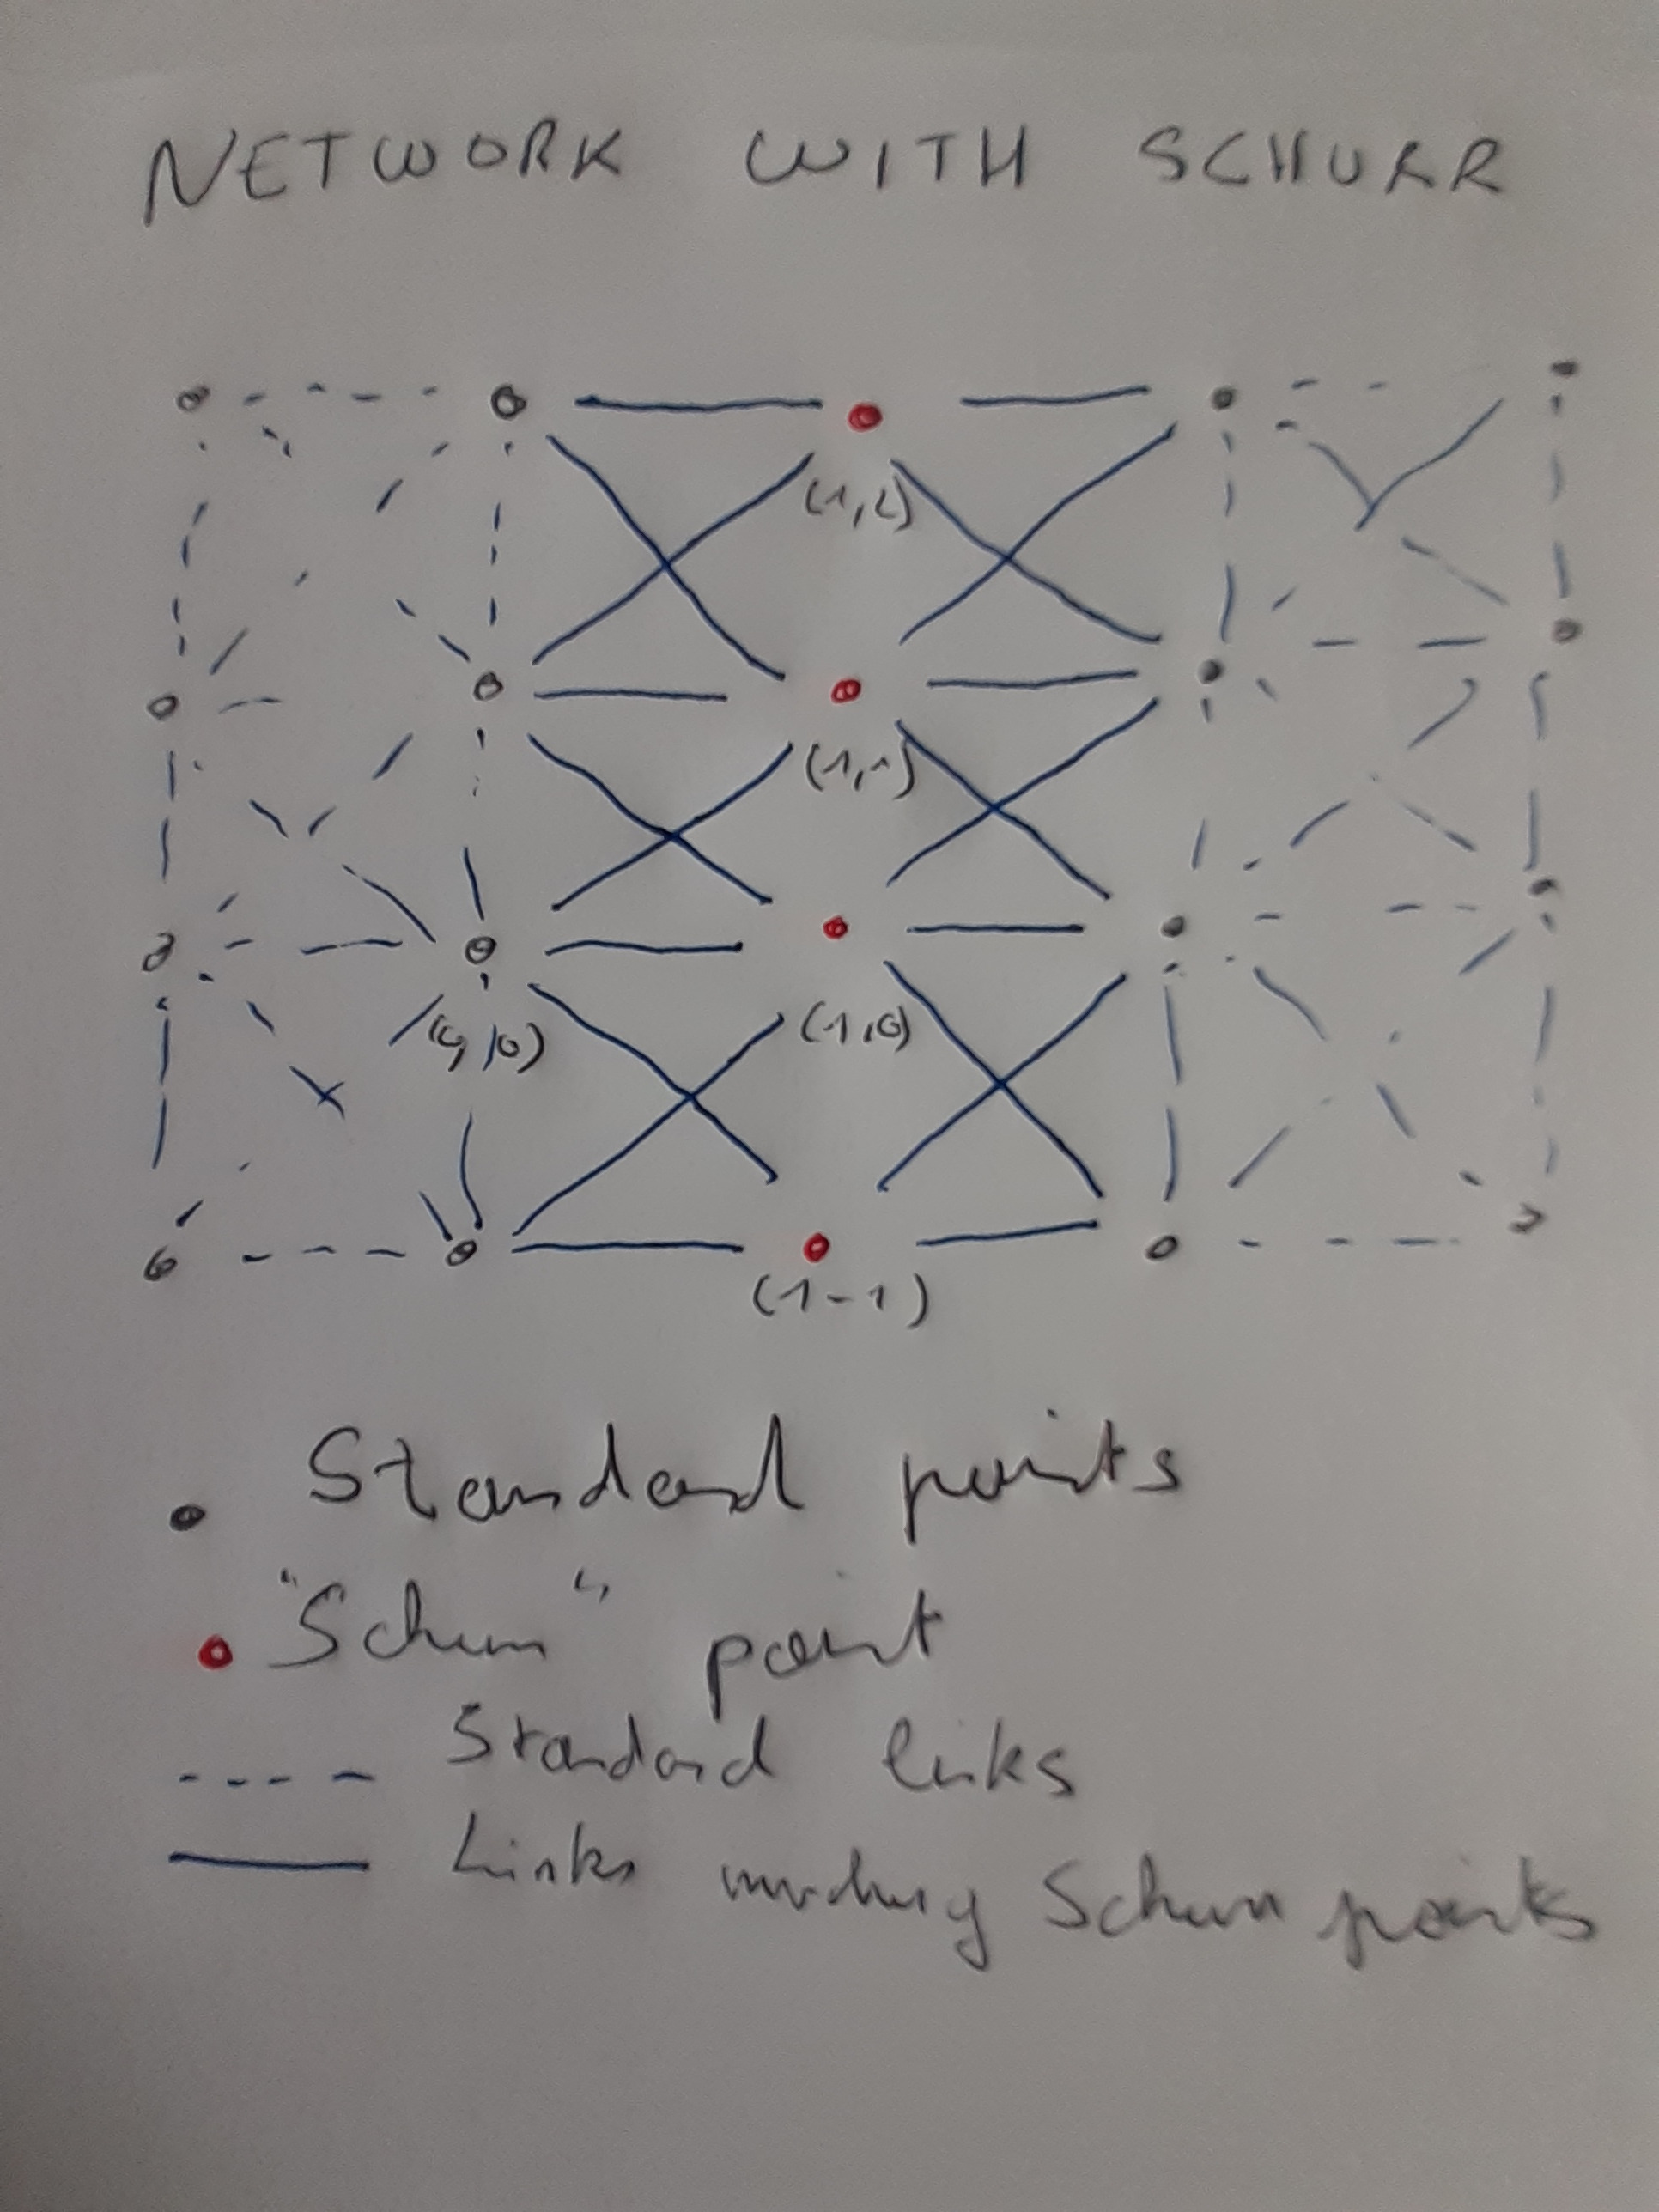
\includegraphics[width=12cm]{Methods/Images/T90-NetSchur.JPG}\caption{Network, case with schur}\label{fig:NetSchur}
\end{figure}

%---------------------------------------------

\subsection{Files of MMVII involved}

We make a quick enumeration of files of MMVII that are to access for understanding :

\begin{itemize}
    \item {\tt include/MMVII\_SysSurR.h} contains the declaration of the class relatives to
          non linear optimisation, from the user point of view the main class
          is {\tt  cResolSysNonLinear};

    \item {\tt src/Bench/BenchResolSysNonLinear.cpp} contains the code for the $2d$-triangulation
          example;

    \item {\tt src/SymbDerGen/Formulas\_Geom2D.h } and {\tt src/SymbDerGen/GenerateCodes.cpp } 
          contains the code for generating the automatic differentiation 

    \item {\tt src/GeneratedCodes/CodeGen\_cDist2DConsVal.cpp } contains the code for 
          generating the automatic differentiation , also it is theoretically not necessary 
          to see it for using it, it's no harm to be curious and not use it as a black box;
          by the way in real case use, it will not be necessary to look at the code that you
          will generate.
\end{itemize}

%---------------------------------------------
%---------------------------------------------
%---------------------------------------------

\section{Computing functions and their derivatives}
\label{Compute:Deriv:SysNL}

%---------------------------------------------
\subsection{Motivation}

For Gauss Newton iteration, in equation \ref{EqNLOInit}, we will need to compute not only
the $f_j$ but also all its partial derivative $\frac{\partial f_j}{\partial x_i}$
relatively to all variable $x_i$ used in $f_j$.  There are many way to do it,
and to be honest  all have  pro and cons:

\begin{itemize}
    \item numerical derivative are the most simple, but they are slow, and can be unacurrate
          when the "small" value are not correctly choosen;

    \item hand crafted derivative are accurate and can be fast, however they can be complicated
          to write for real case formula (like arrise in bundled adjustement) and can be
          a nightmare to maintain when a "small" change occurs in the formulas;

    \item jet derivative, like used it Ceres, are almost as simple to use as numericall, once
          you have the library,  and much faster and accurate as numerical ones; they are much
          easier to use and maintain as  hand crafted ones, but can be also slower than
          handcrafted;

    \item symbolic derivative and code generation, can be a bit more complicated to use
          than jet, especially the first time; however after  this quick learning step
          they are as easy as jets to use,  easy to maintain and, in some case, much
          faster.
\end{itemize}

The solution implemenented in MMVII in based on symbolic derivative with code generation.
This choice was made because it is believed that programmer that will goes into the
core of MMVII have rather high requirement in code efficiency and are ready to pay a
small learning steps.

%---------------------------------------------
%\section{Generating the code}

          %  - - - - - - - - - - - - - - - - - - - 

\subsection{class for specifying the formulas}

In this  example, we have only one formula we need to compute and derivate, it's
the formula of equation~\ref{EqConsDist}.  First introduce a bit of MMVII's jargon  :

\begin{itemize}
   \item in this formula we have two different kind of variables the $P_i$ and $P_j$
         and the $d_{ij}$;
         
   \item for the $P_i$ themselves we have no direct observation , we only have initial value,
         and our target is precisely to compute their values; they will be named {\tt unkowns};

   \item for the $d_{ij}$ we know their values (it could be with some uncertaincy, but that'
         another story) and dont try to compute it, they will be name {\tt observations}.
\end{itemize}

The class {\tt cDist2DConservation} in file  {\tt src/SymbDerGen/Formulas\_Geom2D.h } contains
all the information that are required for generating code. It must define $5$ members :

\begin{itemize}
   \item a contructor, that does nothing for such a basic example

   \item a method {\tt VNamesUnknowns} that return the vector of names of unkown ,
         here we have $2$ points and $2$ coordinates $x,y$ for each points so the
         vector has a length of $4$;  the names will be used for code generation;

   \item a method {\tt VNamesObs} that return the vector of names of observations ,
         here we have a single observation which is the targeted distance between 
         $P_1$ and $P_2$;  the names will be used for code generation;

   \item a method {\tt FormulaName}  that return the name of the formula itself,
         the method will be used for the name of class and files containing the generated
          code;

   \item a method {\tt formula}  this is the core of the class, this method
         take as input a vector of unknown and a vector of observation and return
         a vector that is the result of the  computation  (typically a residual
         when used in context of gauss newton);  the type of {\tt tUk} of the
         i/o vectors and of temporary variable, is not very important at this step,
         it's suffice to know that it is a type on which most current mathematicall
         operation are defined (and can be completed when missing), they represent
         mathematical formula as symbolic tree; see \RefFantome for detailled
         explanation on the type {\tt cFormula<Type>} defined in 

\end{itemize}

Regarding the $3$ methods that  return names, as they are used as \CPP identifier
its important that they contains only valid character (alpha numeric and {\tt\_} ,
no {\tt + - ...}),  also it's important that  inside a vector they are unique.
Apart of that, their exact name is unimportant, but giving names semantically
meaningful is useful if a human want to read the generated code (something we
generally dont do, but something we will do here).

\begin{equation}
      D(X) = \sum_{j=1,M} (\frac{d(P_i-P_j)}{d_{ij}} - 1)^2  \label{EqConsDistHom}
\end{equation}

Regarding the method  {\tt formula}, it's here a direct implementation 
of residual used in  equation~\ref{EqConsDistHom}, which
is non dimensionnal variant of equation~\ref{EqConsDist}. Some comment :

\begin{itemize}
   \item we make an intensive use of the {\tt auto} type specification which
         is convenient here;

   \item the less intuitive part is probably {\tt  CreateCste(1.0,x1);},  in fact
         when we need to create a constant  we must indicate the type of symbolic
         formula to the constant is create with adequate type, the {\tt x1} parameter
         is just used to indicate the type in the template function {\tt CreateCste},
         putting {\tt x2}, {\tt y1} or any other would have exactly the same effect;

   \item the function return a vector of formula, which here is of size $1$, and not
         single value, because in general, when we want to compute several values (like
         $x$ and $y$ residual in BA)  its more efficient and convenient to group 
         a multiple residual in a single formula that generating different formulas;

\end{itemize}

As a slightly more complex example, the reader can investigate example {\tt cRatioDist2DConservation}
in the same file. This example correspond to the case what we want to preserve is not the distances
but the angles or ratio of distance. For each triangle $P1,P2,P3$, we have the initial 
distance $D_{i,j}$ as observation and  we write :

\begin{equation}
      \frac{d(P_i,P_j)}{D_{ij}} - \frac{d(P_i,P_k)}{D_{ik}} = 0 \label{EqRatioDist}
\end{equation}

In this cas we have $3$ equation and the function has $3$  values corresponding to the
$3$ possible combination of  equation~\ref{EqRatioDist}.

          %  - - - - - - - - - - - - - - - - - - - 

\subsection{Generating the code}

Once the class {\tt cDist2DConservation} has been created, the things to do for generating the
code is quite simple :

\begin{itemize}
    \item   add in file  {\tt GenerateCodes.cpp } a call to   the method {\tt GenCodesFormula}
            with an object of type {\tt cDist2DConservation}, note that we call it twice,
            the second boolean parameter indicating if we want to  compute the derivate;
            in fact sometime we will be interested only by the function and will not want
            to pay the price for the derivate;


    \item   compile with {\tt make}, execute a call to {\tt MMVII} command {\tt GenCodeSymDer},
            and compile again.
\end{itemize}


Also it's generally not necessary, we invite here the curious reader to give a look
at generated code.  All the such codes are located in {\tt src/GeneratedCodes/} ,
and here in the files  {\tt CodeGen\_cDist2DConsVal.cpp}, w/o derivative, and 
{\tt CodeGen\_cDist2DConsVDer.cpp}, with derivatives, the declaration of the classes
are in corresponding header file ({\tt CodeGen\_cDist2DConsVal.h} \dots). 
Note that the name used for file ans classes come from the result of {\tt FormulaName}.

Lets make a quick comment on {\tt CodeGen\_cDist2DConsVDer.cpp} :

\begin{itemize}
  \item  the computation is made in a loop {\tt for (size\_t aK=0;....)}, this 
         allow a paralelization of the code when high performance computation is
         required;

  \item  the name used for unkowns and observation can be recoginzed as local
         variable at the begining of the loop;

  \item  after the code is a very monotonous code with basic instructions as
         {\tt Fx = Fy op Fz;}  or {\tt Fx=Op(Fy);}  ,  this is not the way
         human would write code ...  however it is not made to be read and you may
         think of it as "high level assembleur code";

  \item  by the way the code is relatively optmized to avoid multiple redundant computation,
         for example you can see that formula {\tt F8}  that represent {\tt y1-y2} is computed
         once and used three time;

  \item  the result of one iteration contain $5$ value here, because we have the value of the function
         itself and the value of the derivative relative to the $4$ variable ($x$ and $y$ of
         $P_1$ and $P_2$) ;  

  \item  there is a high level interface for extracting independantly value and derivatives,
         but we will not need it here, as everything will be encapsulated in the main 
         class {\tt cResolSysNonLinear};

  \item  give a look at file {\tt CodeGen\_cRatioDist2DConsVDer.cpp}, in this case we have $21$
         values ; $21 = 3 * (1 + 3*2)$ , the ratio return a vector of $3$ values, and
         for each value we compute the value itself and its derivatives relative to the $6$
         variable ($x,y$ for $3$ points), again there is a high level interface for extracting
         these values.
\end{itemize}

          %  - - - - - - - - - - - - - - - - - - - 

\subsection{Creating the object}

\label{CreateCalc}

For computig the value and derivative of {\tt cDist2DConservation} in our \CPP program,
 a possible and classical way is to include the file declaring the class
(i.e. {\tt CodeGen\_cDist2DConsVal.h}) and explicitely create a {\tt cDist2DConsVDer}.

However the optimizer is done to work with any object deriving from the abstract mother
class of all object resulting from code generation :  {\tt cCompiledCalculator<double>};
so the optimizer only manipulate pointers on such class and the exact class is not used.
There is a function for creating an object from its name, and we create an allocator
from this name with the function {\tt  EqConsDist(bool WithDerive,int aSzBuf)}.

The definition in {\tt GenerateCodes.cpp }  is pretty basic :

\begin{lstlisting}
cCalculator<double> * EqConsDist(bool WithDerive,int aSzBuf)
{
    return cName2Calc<double>::CalcFromName(NameFormula(cDist2DConservation(),WithDerive),aSzBuf);
}
\end{lstlisting}


And the declaration in a header file (here {\tt MMVII\_PhgrDist.h} ) :


\begin{lstlisting}
NS_SymbolicDerivative::cCalculator<double> * EqConsDist(bool WithDerive,int aSzBuf);
\end{lstlisting}

Now from the user side, the only thing we need to do is calling  {\tt EqConsDist}. This
correspond in file {\tt BenchResolSysNonLinear.cpp}  to line:


\begin{lstlisting}
     mCalcD =  EqConsDist(true,1);
\end{lstlisting}


%---------------------------------------------
%---------------------------------------------
%---------------------------------------------

\section{Non linear system}

This section was written assuming that the user explicitely controls the numbering of all
the variable because this was the way it was done at the begining. Meanwhile, a mecanism
described in~\ref{SecAutoUkAlloc} has been added to facilitate this automatic numbering.
By the way the explicit numbering is still accessible, because it is believed that the
two mecanisms are useful.

\subsection{Introduction}

The class for solving  non linear system is the template class 
{\tt  cResolSysNonLinear<Type>}. This class provides an easy interface
for computing fonctions and their derivatives (via object resulting from code generation)
and weighted least squares in the aim of solving non linear systems.

The template of the class refers to the way linearized equation are store and solved.
Probably {\tt tREAL8=double}  would be a good default value, while {\tt tREAL16}
could be used when high accuracy is required.

The main operations that can be done with such solver are:

\UNCLEAR
\begin{itemize}
   \item create a solver with initial values of the unknowns and parameters for
          specifying the adjoint least square solver; 

   \item add directly  an equation on subset of unkowns \emph{w/o} temporary unknowns;

   \item add  an equation with a subset of unkowns \emph{with} temporary unknowns  to
         a structure that accumulate them;  then  add this structure to the solver;

   \item add equation fixing a given variable;

   \item acces to current solution;

   \item compute the next current solution and reinitialize the solver.

\end{itemize}


          %  - - - - - - - - - - - - - - - - - - - 

\subsection{Least square solving and constructor}

In {\tt src/TutoBenchTrianguRSNL/cMainNetwork.cpp} the call to these constructors can be found
after tags {\tt  BASIC:CONSTRUCTOR} and {\tt LEASTSQ:CONSTRUCTOR}.
The dense vector is created from a standard vector.\UNCLEAR

In {\tt MMVII} the core calculation of matrix algebra is realized
by eigen library. The services offered by {\tt MMVII} is essentially
an interface for storing data and for a more homegeneous integration
in {\tt MMVII} "philosophy".

In {\tt MMVII} there is several ways to handle least squares systems, each
one correspond to a value of enumeration {\bf \tt eModeSSR} :

\begin{enumerate}

    \item{\bf \tt eSSR\_LsqDense :}
          uses dense matrix for storing the normal matrix; for system not so spare,
          or for small systems, this is the most efficient way; typically if you have
          (many) thousands of limited size systems, this is the mode you must use; solving
          is made by calling \emph{"ldlt"} method of eigen (i.e. Robust Cholesky 
          decomposition of a matrix with pivoting); this classes use schur-complement
          for handling temporay unknowns;

    \item {\bf \tt eSSR\_LsqNormSparse :}
          uses sparse matrix for storing the normal matrix; this is probably the most
          general way and the most efficient in time and storage for most cases in 
          photogrammetry involving many pose estimations. Its
          drawback is that using normal equations increase the conditionning of the
          system, the potential problem increasing with number of unknowns; 
          solving is made calling  {\tt SimplicialCholesky} decomposition of eigen;

    \item {\bf \tt eSSR\_LsqSparseGC :}
          uses sparse representation that memorize all the individual obsertions;
          \emph{do not} use normal equations, the solving is made using
          {\tt LeastSquaresConjugateGradient} decomposition of eigen;
          \emph{do not} use Schur complement for temporary unknowns, they
          are processed like the other unknowns; according to eigen documentation
          this method is the more robust for poorly conditionned systems 
          compared to {\bf \tt eSSR\_LsqNormSparse}, for big
          sparse system with a high proportion of temporary unknowns, 
          it's certainly less memory  efficient and it's probably
          less CPU-efficient (but intensive test remain to be done);

\end{enumerate}

The basic constructor takes an enum value as parameter to specify
the least square solver and an initial value:

\begin{lstlisting}
       cResolSysNonLinear(eModeSSR,const tDVect & aInitSol);
\end{lstlisting}


It is also possible to create a solver with an explicit least square solver.
This is usefull especially with {\bf \tt eSSR\_LsqNormSparse} because the memory
allocation (still in construction) is more complex and may require more parametrisation
from the user.  \UNCLEAR



          %  - - - - - - - - - - - - - - - - - - - 

\subsection{Adding a basic equation}

The tag  {\tt  BASIC:CALC} in {\tt BenchResolSysNonLinear.cpp} contain an example of such use.
The method for adding an observation is named {\tt CalcAndAddObs} :

\begin{lstlisting}
    void   CalcAndAddObs(tCalc * aCalc,const tVectInd & aVI,const tStdVect& aVObs,const tResidualW & aWeighter= tResidualW());
\end{lstlisting}

The $4$ parameters are :

\begin{itemize}
   \item {\tt aCalc} is a calculator as described in~\ref{CreateCalc};

   \item {\tt aVI} is a std::vector of  int that contains the index of unknowns used;

   \item {\tt aVObs} is a std::vector of  {\tt double} that contains the observation;

   \item {\tt aWeighter} is an object used for computing the weight of the observation, 
         the default value  associate a constant weight $1$, we will not discuss more 
         this parameter at this step.

\end{itemize}

What is done is what can be expected :

\begin{enumerate}
   \item  use  vector {\tt aVI} and {\tt aVObs}  to fill the parameters
          of the functor {\tt aCalc}; for {\tt VI} the index are used read the 
          values of the current unknown

   \item  execute the computation of {\tt aCalc} , that must  have been created
          with the {\tt WithDer} option at {\tt true};

   \item  use the result of differentiation and the weighting computed by {\tt aWeighter}
          to add a linearized equation in the least square system.
\end{enumerate}


          %  - - - - - - - - - - - - - - - - - - - 

\subsection{Adding with schur complement}

The tag  {\tt  SCHUR:CALC} in {\tt BenchResolSysNonLinear.cpp} contain an example of such use.
Adding equation with temporary variables, is slightly more complex, as the elimination
can only be done once we have all the equations involving a given subset of unknowns.
So the computation is done in $2$ steps : (1) create a structure, give at this initialisation
step  the current values of unkonws (2) accumulation in a structure 
with {\tt AddEq2Subst}, (3) using this structure
for adding the equation on unknowns after having done the elimination of temporary unknowns with
{\tt  AddObsWithTmpUK}

The structure is {\tt cSetIORSNL\_SameTmp<Type>}, the method for accumulating 
equation has the signature :

\begin{lstlisting}
    void  AddEq2Subst (tSetIO_ST & aSetIO,tCalc *,const tVectInd &,
                       const tStdVect& aVObs,const tResidualW & aWeighter= tResidualW());
\end{lstlisting}

In this method {\tt aVObs} and {\tt aWeighter} are identic to the equivalent in
{\tt CalcAndAddObs}. For the others :

\begin{enumerate}
   \item the first one {\tt cSetIORSNL\_SameTmp<Type>}, is the accumulating structure, it
	   constructor takes current values of temporaries;

   \item  the vector {\tt aVI} contains the  unknown and temporary unkown,  
	   conventionnaly the numbering of unknown is made with negative numbers starting from
           $-1$ to distinguish them from standard unknown, in this example they are $-1$ and $-2$,
           standard unknown are processed as before; 
         s  ee {\tt aVIndMixt} after tag {\tt SCHUR:CALC}

   \item  the vector {\tt aVTmp} contains the  values of temporary unknowns;
\end{enumerate}

Once the equation have been accumulated, it is sufficient to call {\tt AddObsWithTmpUK}
with the structure as parameter.

          %  - - - - - - - - - - - - - - - - - - - 
          %  - - - - - - - - - - - - - - - - - - - 
          %  - - - - - - - - - - - - - - - - - - - 

\subsection{Equation fixing a variable}

          %  - - - - - - - - - - - - - - - - - - - 
\subsubsection{Weigthed version for standard variables}

\label{WeightedFixVar}
The tag  {\tt  EQ:FIXVAR} in {\tt BenchResolSysNonLinear.cpp} contain an example .

It currently happen that the solution we compute is undetermined
up to  certain transformation.  If we do nothing, the least square
system will be not inversible and this will create problems.
A current way  to overcome this difficulty is to fix a set
of arbitrary variables.  In our case, as said in~\ref{Eq:FixVarAB}, 
we fix arbirtrarily $x_A,y_A,x_B$.  

The method {\tt AddEqFixVar} can be used for that, it takes $3$ parameters :
the number $k$ of the var, the value $V$ we want to assign, and the weight $w$
of the equation.  It simply add the following term  to the minimization :

\begin{equation}
      w (X_k -V)^2   
\end{equation}

The variant {\tt AddEqFixCurVar} fix the value of $x_k$ to its current value.

          %  - - - - - - - - - - - - - - - - - - - 

\subsubsection{Rigid fixing of a variable}

Sometime, we want to fix rigidly a variable to a given value.  Doing it with
a very high weight (almost "infinite") using method of~\ref{WeightedFixVar} would not be very 
good idea in general because the notion of very high weight is dependant of the context
and of the "dynamic" of the variable, and setting it to a universally  high value would lead to numerical 
instability.

In this case, the {\tt SetFrozenVar} familly must be used. The way it works is  totally
different of {\tt AddEqFixVar} and is the following :

\begin{itemize}
    \item {\tt MMVII} keep memory of all variable that have been frozen ;
    \item each time a linearized equation is added $\sum a_k X_k = B $ , for
             each $k$ where the variable $X_k$ is frozen to $F_k$ , $a_k$ is set to $0$ and $B$
             is set to $B - a_k F_k$;

    \item   also at the end (before solving) we had the equation $X_k=F_k$ with a weight of $1$
            for each frozen variable.
\end{itemize}

To have a correct behaviour of this "interception" mecanism it is required that all the frozen variable
are known before any equation is added. This constraint is tested by {\tt MMVII} and a dynamic
error will occur if this is not respected (see {\tt AssertNotInEquation}).

There is two method using explicit numbering :
\begin{itemize}
    \item {\tt void  SetFrozenVar(int aK,const  Type \&);} froze to an explicit value;
    \item {\tt void  SetFrozenVarCurVal(int aK);} froze to current value.
\end{itemize}

There exist also a familly of method for using with automatic numerotation, see~\ref{SecAutoUkAlloc}.


          %  - - - - - - - - - - - - - - - - - - - 

\subsubsection{Weighted/Froze, equation fixing a temporary}

\label{FrozeSetIORSNL}

In some case, it may be usefull to add a weighted fix observation  on temporary variable.
For example, if we have some ground observation on $3-d$ points associated to a tie-points.

This can be done, inside the {\tt cSetIORSNL\_SameTmp} with the method {\tt AddFixVarTmp}.

Also it may be useful to freeze the temporay if we want to reuse an existing calculator
in a context where some value are completely known \footnote{of course we could rewrite the
equation and set the unknown as observation, but this may be less convenient}.

This can be done at the creation of {\tt cSetIORSNL\_SameTmp} by adding an optional parameter :
the list of index that are frozen (it is also possible to change the value, but i really do see
why it should be useful !!!).

          %  - - - - - - - - - - - - - - - - - - - 

\subsection{Access to current solution}

There is two methods for accessing to the current solution of the system :

\begin{itemize}
       \item {\tt CurGlobSol()} : return globally the current solution (as a dense vector);

       \item {\tt CurSol(int k)} : return  the current value of $x_k$;

\end{itemize}

          %  - - - - - - - - - - - - - - - - - - - 

\subsection{Compute next iteration}

Once we have accumulated all the observation at a given step, what we classically
want to do is to :

\begin{itemize}
       \item use these observation  to have a better estimation of the solution by solving
             the least square system;

       \item supress  these observations of the system (reset it) because, due to linearisation,
             they were approximation, and we expect now to have a better approximation;

       \item use the computed solution in the next iteration as estimation for the linearization.
\end{itemize}

This is done by the method {\tt SolveUpdateReset() ;}.

%---------------------------------------------
%---------------------------------------------
%---------------------------------------------

\section{Image, optmization and differenciation in MMVII}

          %  - - - - - - - - - - - - - - - - - - - 
\subsection{Introduction}

In this section we present the facilities offered in MMVII when we want to mix non
linear optimisation with images. Typically example of such use are :

\begin{itemize}
     \item computing a deformation that transform a model of form  to an image;
           this is (will be) used  in MMVII for refining the  geometry of coded target detection;
           a very similar example, occurs in optical caracter recognition, if we know the font,
           the matching between a potential detectected character and the model ("Ab\'ec\'edaire" in french);

      \item this will/could be used (maybe) in matching method that used deformable mesh for modeling
            the geometry between different images (a well known variant being least-square matching);

      \item this could be used for deformable contour (a topics that used to be very active in 
            pattern recognition).
\end{itemize}

          %  - - - - - - - - - - - - - - - - - - - 
\subsection{Mathematical modelization}

The basic mathematical modelization is simply to consider images as functions.
As we deal with  continuous optimization, we need to have an interpolation scheme that
allow to consider them as function from $\RR^2 \rightarrow \RR$.
Ideally (to be mathematically consistant with derivation) we should use an interpolation 
model that is continuously derivable as bicubic interpolation. Also for efficiency reason,
we will generally prefer a non rigourous model as bilinear;  however the redundancy generally make
neglectable the difference with bicubic (probably, later, the bicubic option will be added for finer
tests).

A typical example is:

\begin{itemize}
      \item we have an image $I$, we note $I[i,k]$ its value for integer points;
      \item we extend  $I$ to a function $\RR^2 \rightarrow \RR$ via the interpolation;
      \item we have a mapping of  $\RR^2$,  $\phi : \RR^2 \rightarrow \RR^2$.
      \item we want to use the composed function $I \circ \phi$;
\end{itemize}

Let $p$ be a point and $q=(\tilde{x}_q,\tilde{y}_q)=\phi(p)$ its transformation by $\phi$. Let $x_0$ and $y_0$
be the lower bound of $q$, and $x_1=x_0+1, y_1 = y_0+1$:

\begin{equation}
	x_0 \leq \tilde{x}_q < x_1   \; and \;  y_0 \leq \tilde{y}_q < y_1
\end{equation}

Almost everywhere \footnote{except for integer values of $\tilde{x}_q,\tilde{y}_q$ }, 
the value of $I \circ \phi$ in a neighourhood of $p$ with  bilinear
interpolation is given by :

\begin{equation}
	I(\phi(p)) =   (x_1-\tilde{x}_q)(y_1-\tilde{y}_q) I[x_0,y_0]  
	             + (\tilde{x}_q-x_0)(y_1-\tilde{y}_q)I[x_1,y_0] \dots 
		     \label{Eq:Bilinear}
\end{equation}

We see with equation~\ref{Eq:Bilinear} that we don't need to add new primitive to compute $I \circ \phi$,
as it just a polynomial combination of existing primitives. By the way, reprogramming it
each time we need it would be fastidious and MMVII offers facility functions to make the use of 
formula~\ref{Eq:Bilinear}  easier.

          %  - - - - - - - - - - - - - - - - - - - 
\subsection{Facility functions}

\subsubsection{For code generation}

The facility functions are defined in the file {\tt "include/MMVII\_TplSymbImage.h"}. Note that this file 
must be explicitely included as it is not included by default in the library.

The template function {\tt FormalBilinIm2D\_Formula} is a direct implementation of equation~\ref{Eq:Bilinear}.
It will be used in the function generating code when we need things like $I \circ \phi$.
It takes two kind of parameters :

\begin{itemize}
   \item the parameters {\tt FX} and {\tt FY} correspond to function $\phi$ :  
	  {\tt FX $\sim \tilde{x}_q$} and {\tt FY $\sim \tilde{Y}_q$}, 
         they will be of type formulas; 

   \item the parameter {\tt aVObs}  corresponds to formula for the observations of equation~\ref{Eq:Bilinear},
         it contains $6$ values $x_0,y_0, I[x_0,y_0] \dots$ .
\end{itemize}

Fonction {\tt FormalBilinIm2D\_NameObs} just generate a vector of $6$ names, it use is recommande for standardizing generated code.
Note that it takes a prefix added to  each name, it will be useful in case we need to use several image in the same
formula to avoid name clash in generated code.
	

\subsubsection{For using generated code}

When using code generated, we need to fill the value of observation with values    $x_0,y_0, I[x_0,y_0] \dots$
in a given context.  The function {\tt FormalBilinIm2D\_SetObs} can be used to facilitate this filling .
More important it must be used to warantee the coherence of ordering with  {\tt FormalBilinIm2D\_Formula}.
The parameter are :

\begin{itemize}
    \item {\tt aVObs } is the vector to fill, {\tt K0} is the first index where filling begin;
    \item {\tt aPtIm}  is the point where want to evaluate $I$;
    \item {\tt aDIm}  is the image;
\end{itemize}


%---------------------------------------------
%---------------------------------------------
%---------------------------------------------

\section{Test example for image differenciation in MMVII}

In this section we describe a test example, that has been implemented in MicMac, this example 
has two objective : (1) make a didactic illustration of the fonctionnalities and (2) 
be usable in the automatic test of MMVII ("proof" of correctness and no regression).

\subsection{Mathemical problem}

We have :

\begin {itemize}
    \item a model $M$  function, this model function can be given by an analytic  formula or by a model image;
          in our case it will be a gaussian function;

    \item a parametric transformation of the model, here it is both geometric and radiometric;

    \item a ground truth for the parameters (used for generation and testing, ignored in computation);

    \item an image that contain the transformation of the model with the ground truth parameter;

    \item an initial guess of the parametric transformation, this guess being sufficiantly close to the
	    truth (whatever means "sufficiantly close");

     \item given the model, the image and the initial guess we want to recover the "exact" parameters of the 
           transformation.

\end {itemize}

For the model, we use  a smooth function to have an easy convergence (we dont want to 
make a theoretical analysis of robustness, just illustrate and test implementation).
More precisely we use a gaussian fonction :

\begin{equation}
	M(x,y) =  e^{-\frac{|p-\mu|^2}{\sigma^2}}
\end{equation}

The  parameter of transformation has 5 value :  $P=\{A,B,S,T_x,T_y\}$, where $\{A,B\}$ parametrises
the radiometric homotethy,  and $\{S,T_x,T_y\}$ parametrises the geometric homotethy.
So that :

\begin{equation}
	I[i,j] =  B + A * M(T_x + S*i,T_y+S*j) , (i,j) \in \NN^2  \label{EqDefIm}
\end{equation}

Knowing approximate guess  $\{A',B',S',T'_x,T'_y\}$, the model, the image and equation
\ref{EqDefIm} we want to recover "exact" value of $P$.

Note that we will use equation ~\ref{EqDefIm} in the invert sense of geometry, noting
the parameter of invert homothety $\{\tilde{S},\tilde{T}_x,\tilde{T}_y\}$:

\begin{equation}
	I(\tilde{T}_x + \tilde{S}*x,\tilde{T}_y + \tilde{S}*y) =  B + A * M(x,y) \label{EqDefImInv}
\end{equation}

So what we will estimate is $\{A,B,\tilde{S},\tilde{T}_x,\tilde{T}_y\}$,


\subsection{Generating the code}

The code for generating the automatic derivation applied to the example are located in two files:

\begin{itemize}
    \item {\tt src/SymbDerGen/FormulasImagesDeform.h } contains the definition of  class 
              {\tt cDeformImHomotethy} that will be used for generating the code, it is the homologous
              of class  {\tt cDist2DConservation} seen bellow;

    \item {\tt src/SymbDerGen/GenerateCodes.cpp} , as bellow, contains the code generate the code
          creating calculator;

\end{itemize}

There is no much commentary to do on the code of {\tt cDeformImHomotethy} who
should be explicit given previous section of this chapter.
Just focus on the point specific to bilinear interpolation :

\begin{itemize}
	\item for {\tt VNamesObs} we use the standard names of observation on bilinear 
              and add $3$ name specificto the model;

      \item for computing bilinear interopation of $I \circ \phi$ we use {\tt FormalBilinIm2D\_Formula};

      \item else the computation done in {\tt cDeformImHomotethy::formula()} is a direct "traduction"
	      of equations~\ref{EqDefImInv} and~\ref{Eq:Bilinear}.

\end{itemize}


\subsection{Using the generated code}

The file using the generated code for doing optimization can be found in 
{\tt src/Bench/BenchTutoImageDef.cpp}.  The main class is {\tt cTestDeformIm},
it main action are done in the constructor and the medthod {\tt OneIterationFitModele}.

The main action of constructor {\tt cTestDeformIm} are :

\begin{itemize}
    \item  inialize the ground truth homotethy and its inverse ({\tt mGT\_I2Mod} and {\tt mGT\_Mod2Im};
    \item  inialize the gaussian law in image an model geometry ( {\tt mGaussIm}  and {\tt mGaussModel});
    \item  initialize the image  in {\tt mIm}; 
    \item  put in vectors a set of point $P$ in model space and their associated value $M(P)$
           ({\tt mVPtsMod} and {\tt mValueMod});
\end{itemize}


In {\tt OneIterationFitModele} we parse all the point of the model, and for each point we
add an obsevation corresponding to equation~\ref{EqDefImInv}.

%---------------------------------------------
%---------------------------------------------
%---------------------------------------------

\section{Mechanism for automatic unknown allocation}

\label{SecAutoUkAlloc}

%---------------------------------------------

\subsection{General principle}

This section present a mecanism for automatizing the mecanism of variable numbering in 
equation solver; this mecanism can be especially interesting when the same objects 
appears in different kind of problem.

The general priniciple is :

\begin{itemize}
     \item all the object that have unknowns must inherit from the class {\tt cObjWithUnkowns};

     \item this object must describe their unknown as interval of {\tt double*};

     \item  all the object of a same solver must be accumulated in an object of the class
            {\tt cSetInterUK\_MultipeObj};

      \item once this is done, the class offer many facility for communicating with a solver.
     
\end{itemize}

%---------------------------------------------

\subsection{Class {\tt cSetInterUK\_MultipeObj}}

This class organizes the "coordination" between all object that will participate to the same solver.
The main method usable are :

\label{cSetIUK}

\begin{itemize}
    \item  {\tt  AddOneObj(cObjWithUnkowns<Type> * Obj);} , that must be called once with each object \emph{Obj},
           that has unknowns involved in the solver, the \emph{Set} will memorize the \emph{Obj},
           will make some initialization on  \emph{Obj} and then will call    the
           {\tt PutUknowsInSetInterval} on  \emph{Obj} 

    \item  {\tt  AddOneInterv} where an \emph{Obj}  will indicate its unknowns interval,
          this method will be  called by  \emph{Obj} inside its {\tt PutUknowsInSetInterval};
          the base methods take an adress {\tt double *} and a number, the other are
          just facility that recall this base method;
          
    \item  {\tt GetVUnKnowns}  return a vector of all the unknons and can be used to create a solver
           by giving the initial values;

    \item  {\tt SetVUnKnowns}  modify all the unknown with a vector (typically resulting from
           next iteration of the solver), will also call the method {\tt OnUpdate()} on all its \emph{Obj}.
\end{itemize}



%---------------------------------------------

\subsection{Class {\tt cObjWithUnkowns}}

\label{ClassOWU}

This is the base class for all object that will benefit from automatic ordering. It must override
the pure virtual method {\tt PutUknowsInSetInterval}, when this method is called by a set :

\begin{itemize}
   \item the protected field {\tt mSetInterv} will have been initialized 
   \item the object has just to call {\tt mSetInterv->AddOneInterv} with its unkonwn;
\end{itemize}

The other useful methods defined in the classe are :

\begin{itemize}
   \item    {\tt void PushIndexes(std::vector<int> \& VI);}  add the indexe of unknowns in  {\tt VI}
            for used to add an equation in the solver (as with {\tt CalcAndAddObs}));

   \item    {\tt OnUpdate()}, this virtual call back, will be used after the  object has been
            modified by   {\tt SetVUnKnowns} .

\end{itemize}

There is different method to access to the underlying numerotation of variables
({\tt IndOfVal, IndUk0} \dots) but the method are to be use by solver and their
use directly by the "end-programmer" is not recommanded.

Instead of accessing directly to the numerotaion, the class {\tt cResolSysNonLinear}
 offers different facility freezing  variable , they  take an object and the adress to freeze.
See {\tt void  SetFrozenVar(tObjWUk \& anObj,const  Type \& aVal)} and after.

%---------------------------------------------
%---------------------------------------------
%---------------------------------------------

\section{An Example  with bundle adjusment}

\subsection{Global presentation}

We take the example of two classes where this mecanism is used ,
{\tt cPerspCamIntrCalib} for representing internal calibration of central pesrpective
camera, and {\tt cSensorCamPC}  for representing the pose of camera (contains
the pose itself + a refererence to the calibration).
These two classes are derivates classes of {\tt cObjWithUnkowns<tREAL8>}.

The code corresponding can be found in :

\begin{itemize}
   \item {\tt MMVII\_PCSens.h} for declaration of classes;

   \item {\tt cSensorCamPC.cpp}  and {\tt cCentralPerspCam.cpp} for definition of classes;

   \item {\tt cConvCalib.cpp}  that contain  class {\tt cCentralPerspConversion}.
\end{itemize}


We will study with more detail the class {\tt cCentralPerspConversion}, the purpose
of this class is to create a perspective camera from  as set of $3d-2d$ correspondance.
This is done by a bundle adjusment using colinearity equation where internal and
external parameter are optimized to fit the observations.
Note that this class is used in two different context :

\begin{itemize}
   \item first to do real conversion,  it is used for example by the command {\tt OriConvV1V2}
   \item second  it is use ti make test/bench; 
\end{itemize}

In second case, we generate artificially difficult condition : noisy initialization, but
also we dont give to the system all the information we have, but a sufficient subset, to
check that it still converge to the good solution. This is controled by two boolean
variable that are set to true in real conversion: 

\begin{itemize}
   \item {\tt  mFGC}   indicate if $3d$ are frozen, as it could be with $100\%$ reliable ground control point
                       
   \item {\tt mCFix} indicate is center of camera is frozen;
\end{itemize}


%---------------------------------------------
\subsection{Camera classes viewpoint}


\subsubsection{Class {\tt cSensorCamPC}}

The unknowns that are specific to a pose are the center  and  the rotation (coded as an axiator $\omega$ ).
The  formalisation is that the unknon rotation is the product of the currant rotation
and the a small rotation corresponding to the axiator ($X \rightarrow X + \omega\; \hat{}\; X$).
So, as a    {\tt cObjWithUnkowns<tREAL8>} the cSensorCamPC overrides {\tt PutUknowsInSetInterval} :

\begin{lstlisting}
void cSensorCamPC::PutUknowsInSetInterval()
{
    mSetInterv->AddOneInterv(mPose.Tr());
    mSetInterv->AddOneInterv(mOmega);
}
\end{lstlisting}

Be aware that the order in which we add these unknown has to be coherent with their use in calculator.
Also once the system has evolved, we still to udate $\omega$  and the current rotation
so that the unkwon rotation coded by $\omega$  remains "tiny". This is done  by
overriding {\tt OnUpdate} :


\begin{lstlisting}
void cSensorCamPC::OnUpdate()
{
     mPose.SetRotation(mPose.Rot() * cRotation3D<tREAL8>::RotFromAxiator(-mOmega));
     mOmega = cPt3dr(0,0,0);
}
\end{lstlisting}

\subsubsection{Class {\tt cPerspCamIntrCalib}}

The unknown specific to internal calibration of a central perspective camera are focal, principal 
point and parameters of distorsion. 


\begin{lstlisting}
void cPerspCamIntrCalib::PutUknowsInSetInterval()
{
    mSetInterv->AddOneInterv(mCSPerfect.F());
    mSetInterv->AddOneInterv(mCSPerfect.PP());
    mSetInterv->AddOneInterv(VParamDist());
}
\end{lstlisting}

If the camera is modified, the pseudo inverse is no longer valid, so we have to update it :

\begin{lstlisting}
void cPerspCamIntrCalib::OnUpdate()
{
    mInv_CSP       = mCSPerfect.MapInverse();
    if (mInvApproxLSQ_Dist!=nullptr)
       UpdateLSQDistInv();
}
\end{lstlisting}

\subsection{Detailled comment}

The code of {\tt cConvCalib.cpp} has been tagged with several commentary begining by {\tt \#DOC}.
We now describe the link between these tags and several sections of this chapter :

\begin{itemize}
    \item  {\tt  \#DOC-AddOneObj} describe the insertion of object with unknown in a coordinator
           as described in~\ref{cSetIUK};

    \item  {\tt  \#DOC-GetVUnKnowns} describe how we can extract a vector of unknowns
           from the coordinator, as described in~\ref{cSetIUK}, and use it to create a solver;

    \item {\tt   \#DOC-FixVar} describes freezing of some variable of an object as described in~\ref{ClassOWU};

    \item {\tt  \#DOC-PushIndex} describes how to complete the vector of indexes as describes in~\ref{ClassOWU};

    \item {\tt \#DOC-FrozTmp } describes how the value of temporary variable can be frozen using the
          constructor of {\tt cSetIORSNL\_SameTmp} as described in~\ref{FrozeSetIORSNL};
          in this example we freeze the $3$ coordinate of the point, this allow to use the same
          collineraity equation with tie points and ground control points.

    \item {\tt  \#DOC-SetUnknown} describes how we use the result of one iteration of the solver
          to modify all the object handled by the coordinator.

\end{itemize}

%---------------------------------------------
\subsection{Recommandation and limitation}

It is hope that the mecanism will significatively simplify the use of solver.

It is highly recommanded that inside the same solver, the developper does nor mix the two
mode (explicit and implicit numerotation);

A current limitation is that an object can belong only simultaneously to one coordinator.
If we need to change the coordinator the object, which can often happens, the coordinator 
must be destroyed (because at the destruction all object are reset from their link to the
coordinator). If the need arrise to have simultaneous  coordinator, there is possible solution,
then contact MPD.



%---------------------------------------------
%---------------------------------------------
%---------------------------------------------

\section{Topometric compensation (WIP)}

\subsection{Global presentation}

The premises of a topometric compensation system can be found in \texttt{MMVII/src/Topo/}.

Computation takes place in a 3D cartesian frame. For now, there is no georeferencing
and no Earth model.

All points must be given approximative coordinates as there is no automatic initialization.

For now it is only used in the Bench \texttt{TopoComp}.
This Bench will be used to illustrate the topometric classes and their usage.


\subsection{\texttt{TopoComp} Bench example}
\label{subsec:topoBench}

The example is created by the method \texttt{cTopoComp::createEx1()}.

\subsubsection{Step 1}

At first, there are 3 fixed points ($A$, $B$, $C$), forming an isosceles triangle
on an horizontal plane (Fig. \ref{fig:topoEx1}).

\begin{figure}[!h]
\centering
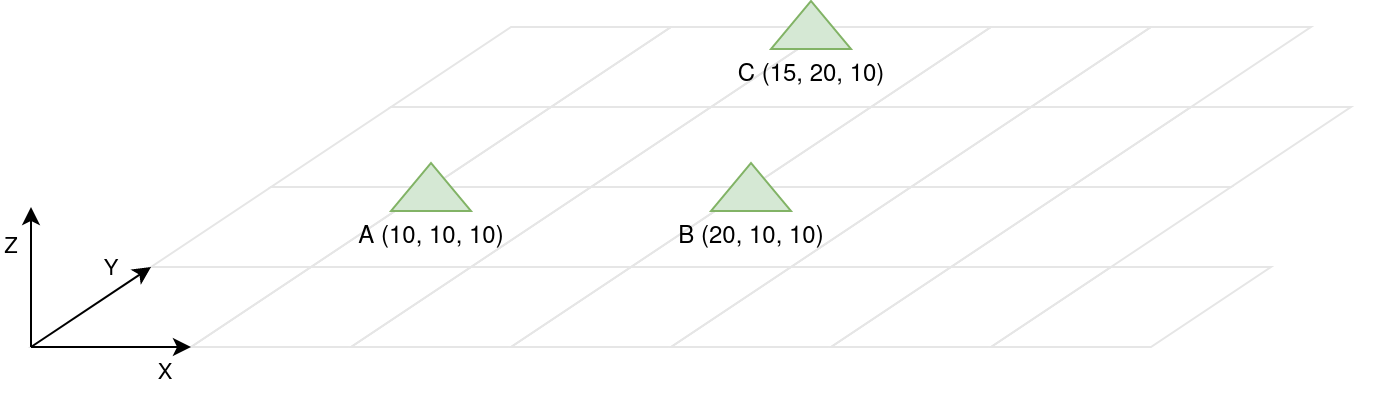
\includegraphics[width=12cm]{Programmer/benchtopo1.png}
\caption{The 3 fixed points}
\label{fig:topoEx1}
\end{figure}

The points are instances of the \texttt{cTopoPoint} class that
derives from \texttt{cObjWithUnkowns}, hence it has no copy constructor and
the points have to be added as pointers to \texttt{cTopoComp::allPts()}.

\begin{lstlisting}
  //create fixed points
  allPts.push_back(new cTopoPoint("ptA", cPt3dr(10,10,10), false));
  allPts.push_back(new cTopoPoint("ptB", cPt3dr(20,10,10), false));
  allPts.push_back(new cTopoPoint("ptC", cPt3dr(15,20,10), false));
  auto ptA = allPts[0];
  auto ptB = allPts[1];
  auto ptC = allPts[2];
\end{lstlisting}

At this point, there are no unknowns and no observations.


\subsubsection{Step 2}

A fourth point ($D$), this time not fixed, is initialized above the $ABC$ triangle.
Distances from $A$, $B$ and $C$ to $D$
are measured. For redondancy and error evaluation, the distance from $C$ to $D$ is measured twice
with different values (Fig. \ref{fig:topoEx2}).

\begin{figure}[!h]
\centering
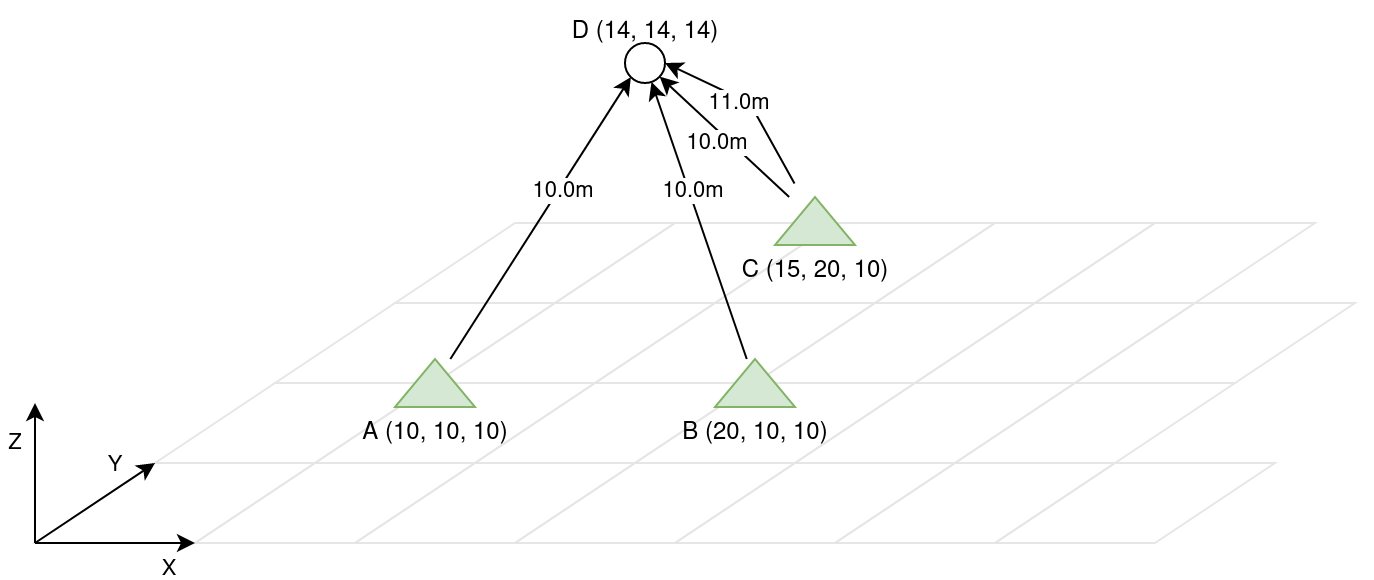
\includegraphics[width=12cm]{Programmer/benchtopo2.png}
\caption{Point $D$ is determined by measured distances}
\label{fig:topoEx2}
\end{figure}

Observations must refer to an observation set (deriving from class \texttt{cTopoObsSet})
that is used to share parameters between observations.

In the case of measured distances there is no parameter, therefore the observation set will be 
a \texttt{cTopoObsSetSimple}. Observations sets must be created with \texttt{make\_TopoObsSet} template function.

All topometric observations are instances of \texttt{cTopoObs} class.
For distances observations, \texttt{TopoObsType::dist} is given to the constructor.

\begin{lstlisting}
  //add measured dist to point D
  allObsSets.push_back(make_TopoObsSet<cTopoObsSetSimple>());
  auto obsSet1 = allObsSets[0].get();
  allPts.push_back(new cTopoPoint("ptD", cPt3dr(14,14,14), true));
  auto ptD = allPts[3];
  cTopoObs(obsSet1, TopoObsType::dist, std::vector{ptA, ptD}, {10.0});
  cTopoObs(obsSet1, TopoObsType::dist, std::vector{ptB, ptD}, {10.0});
  cTopoObs(obsSet1, TopoObsType::dist, std::vector{ptC, ptD}, {10.0});
  cTopoObs(obsSet1, TopoObsType::dist, std::vector{ptC, ptD}, {11.0});
\end{lstlisting}

The system now contains 3 unknowns ($D$ coordinates) and 4 observations
(measured distances $AD$, $BD$ and $CD$ two times).

\subsubsection{Step 3}

A second non-fixed point, $E$, is initialized inside the $ABCD$ tetrahedron,
and observations expressing that
the distances from $E$ to $A$, $B$, $C$ and $D$ are equal and unknown ($d$ in Fig. \ref{fig:topoEx3})
are added.

\begin{figure}[!h]
\centering
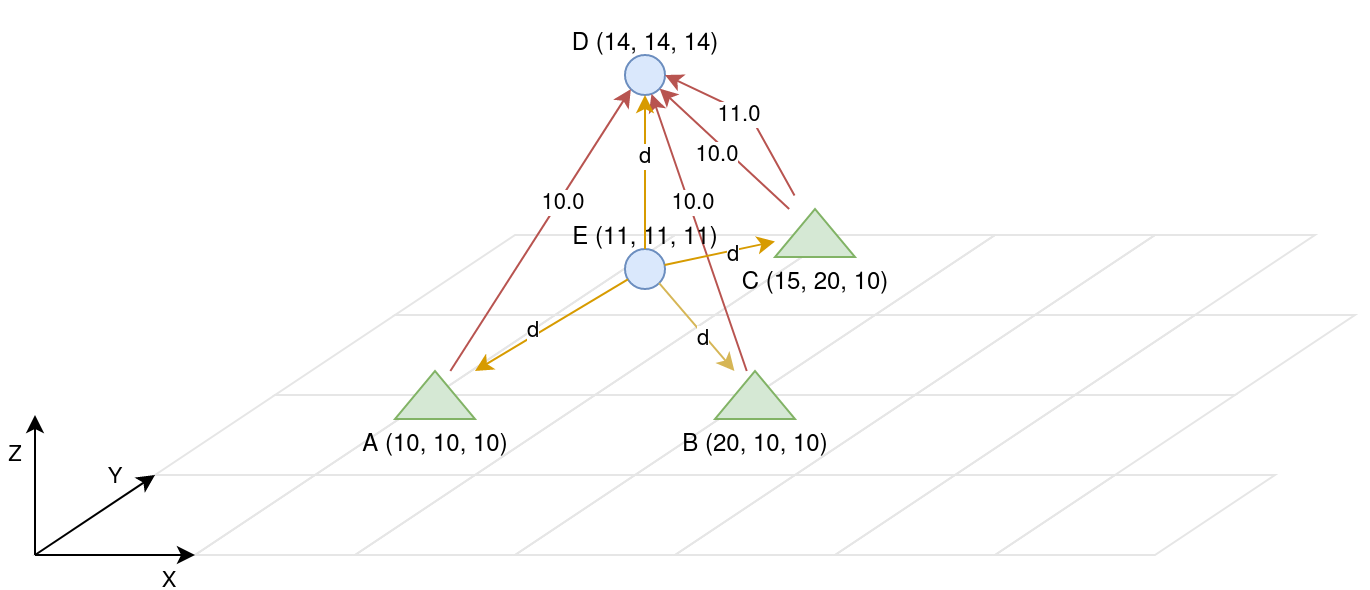
\includegraphics[width=12cm]{Programmer/benchtopo3.png}
\caption{Point $E$ determined by equal distance $d$}
\label{fig:topoEx3}
\end{figure}

A new \texttt{cTopoObsSet} must be created. The \texttt{cTopoObsSetDistParam} class
is used to create the parameter corresponding to the unknown $d$.


\begin{lstlisting}
  //add point E to an unknown common dist
  allObsSets.push_back(make_TopoObsSet<cTopoObsSetDistParam>());
  auto obsSet2 = allObsSets[1].get();
  allPts.push_back(new cTopoPoint("ptE", cPt3dr(11,11,11), true));
  auto ptE = allPts[4];
  cTopoObs(obsSet2, TopoObsType::distParam, std::vector{ptE, ptA}, {});
  cTopoObs(obsSet2, TopoObsType::distParam, std::vector{ptE, ptB}, {});
  cTopoObs(obsSet2, TopoObsType::distParam, std::vector{ptE, ptC}, {});
  cTopoObs(obsSet2, TopoObsType::distParam, std::vector{ptE, ptD}, {});
\end{lstlisting}

This adds 4 unknowns ($E$ coordinates and the unknown distance $d$) and 4 observations
($EA = EB = EC = ED = d$).


\subsection{Topometric computation}

Topometric computation system is managed by the \texttt{cTopoComp} class.
This handles the list of points and observation sets, the non-linear system
(\texttt{cResolSysNonLinear}), and a mechanism to link the observations to
the automatic derivation system.

After \texttt{cTopoComp} object creation and filling (see \ref{subsec:topoBench}),
the method \texttt{OneIteration()} is called to improve parameters estimation.



\chapter{Symbolic Derivation}

We give a detailled description of how automatic differentiation is handled in {\tt MMVII}.
This description is for programmer who will have to maintain this part or possibly also for curious readers .
However we recommand to read before the short introduction given in~\ref{Compute:Deriv:SysNL} (or better all chapter~\ref{Chap:NLO}) to
have a better understanding of where we go.

For devlopper that will only be users of these  automatic differentiation facilities in {\tt MMVVII} , probably
~\ref{Compute:Deriv:SysNL} or~\ref{Chap:NLO} is sufficient.


%-----------------------------------------------------
%-----------------------------------------------------
%-----------------------------------------------------

\section{introduction}


%-----------------------------------------------------
\subsection{Motivations}

The computation of derivatives of a given function is a central point in metrology
where it is used in Gauss-Newton-like iteration.  There is basically $4$ methods
for computing derivatives :

\begin{itemize}
    \item  computing "by hand", i.e a human apply the rules of derivation as
           learned at school;  for small formula, this method is perfectly manageable 
           and also probably the fastest when the code is optimized;
           but with "complicated" function, as colinearity equation with many distorsion parameters,
           it is error prone, difficult to maintain, and potentially not so fast as there
           are simplifications that human may miss;

    \item  numericall derivative: for example with a $2$ variables function, we use equation as~\ref{NumDer}
           where $\epsilon_x$ is a "small" value relative to variable $x$;
           this method has the advantage of simplicity, if you know the function you know its derivatives;
           it has $2$ drawbacks :  first issue, it's not always easy to define a good small value, a too small value
           creates numericall problem, not enough small is unacurate, all the more with heterogeneous variable the "small"
            value must be re-defined for each variable;  second issue, it is relatively slow, with $N$  variables
           we must have $2N$ evaluations of $F$;

     \item jet method as used in CERES, see~\cite{CERES} for detailled description, it's not error
           prone as "hand crafted", there is no problem of accuracy, they are faster than 
           numerical derivatives; however they are relatively slow compared to formal methods;

   \item formal method, that "more or less" do the same thing than "human computation" (generate the
	   analyticall formula) but do
           it automatically; they are separated between automatic differenciation that analyse the code of a programm
           and symbolic differenciation that construct a tree representation, but to our mind this separation
           is a bit artificial : they are conceptually close and 
           their performance are similar;  {\tt MMVII} uses symbolic differenciation;
           the use is a bit more complicated than jet but can be significatively faster  on complicated
           formulas.
\end{itemize}

\begin{equation}
    \frac{\partial F(x_0,y_0)}{\partial x} \approx \frac{F(x_0 + \epsilon_x,y_0) - F(x_0-\epsilon_x,y_0)}{2* \epsilon_x}
     \label{NumDer}
\end{equation}

%-----------------------------------------------------
\subsection{Code localization}

The code on automatic differenciation has been organized in such a way that 
the code can be reused outside the {\tt MMVII} library. It's a header only code
that is located in {\tt MMVII/include/SymbDer/}.


The code that use it more specifically for task adressed in  {\tt MMVII},
as photogrammetry or compensation in general, are to be found in the
folder  {\tt MMVII/src/SymbDerGen}.


%-----------------------------------------------------
\subsection{Tree/DAG representation}

\begin{figure}
\centering
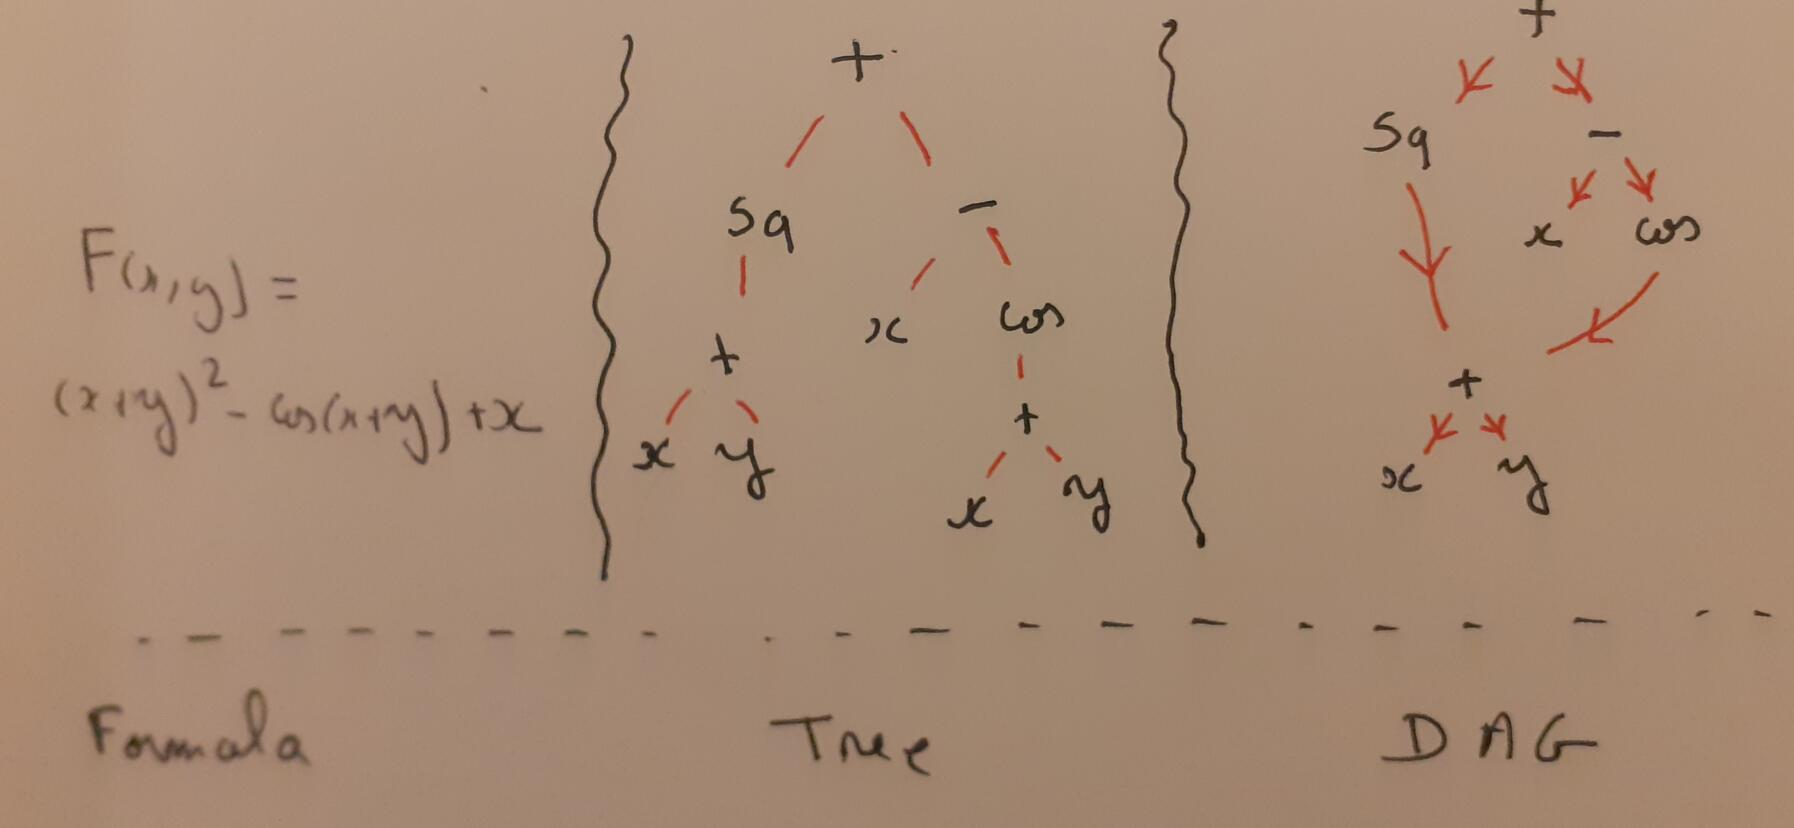
\includegraphics[width=12cm]{Programmer/ImagesProg/Tree.jpg}
\caption{Representation of formulas}
\label{fig:TreeFormula}
\end{figure}

A classic aproach in computer science is to represent mathematicall formulas 
as trees (or more precizely as we will see as "DAG"=  directly acyclic graph).
These trees can be described recursively :

\begin{itemize}
   \item  constant ($0,1,\pi \dots$)  and fonctions corresponding to variables ($x_1,x_2,\dots ,x_{144} \dots$)
          are  atomic formulas, their tree has one node labeled by the contant or the variable;

   \item if $Op$ is a unary operator, like $\cos, \sin, \exp $ for example,  and $F$ is a formula then $Op(F)$ is a 
         formula, its tree is a node labeled by $Op$ and has one son corresponding to the tree of $F$;

   \item if $Op$ is a binary operator, like $+,*,pow $ for example,  and $F_1$  and $F_2$ are 
	   formulas then $Op(F_1,F_2)$ (or $F_1 Op F_2$ in infix notation) is a 
         formula,  its trees is a node labeled by $Op$ and has two son corresponding to the trees of $F_1$ and $F_2$.
\end{itemize}


Figure~\ref{fig:TreeFormula} represent the tree for the formula $F(x,y) = (x+y)^2 +x - \cos(x+y)$. 
In the formula, we see that the sub-formula $x+y$ appears twice , then to optimize the computation,
a directed acyclic graph (DAG) is prefered to tree;  a DAG  is still a hierarchy, but the difference
if that a node can have several parents, which avoid duplication as the same formula can be shared.
The right part of figure~\ref{fig:TreeFormula} correspond to DAG for formula $F$.
When we will generate the code, we will set a variable on the shared node, for example $V_{577} = x+y$ , and then reuse
this variable when we need it instead of redoing computation.


The difference in efficiency between a tree and a DAG can be very significant 
in complicated multiple formula  (maybe up to $10$ in colinearity). By multiple formula we mean formula that return several values;
in differenciation we will compute $F$ but also all its derivatives and it often happen that
the same sub-formula appears in several partial derivatives.  In our example we
have $\frac{\partial F}{\partial x} = 2*(x+y) -1 + \sin(x+y)$ and $\frac{\partial F}{\partial y} = 2*(x+y) + \sin(x+y)$ ,
and figure~\ref{fig:DagMultiformula} represents the DAG for the multiple formula
$\{F,\frac{\partial F}{\partial x},\frac{\partial F}{\partial y}\}$.



\begin{figure}
\centering
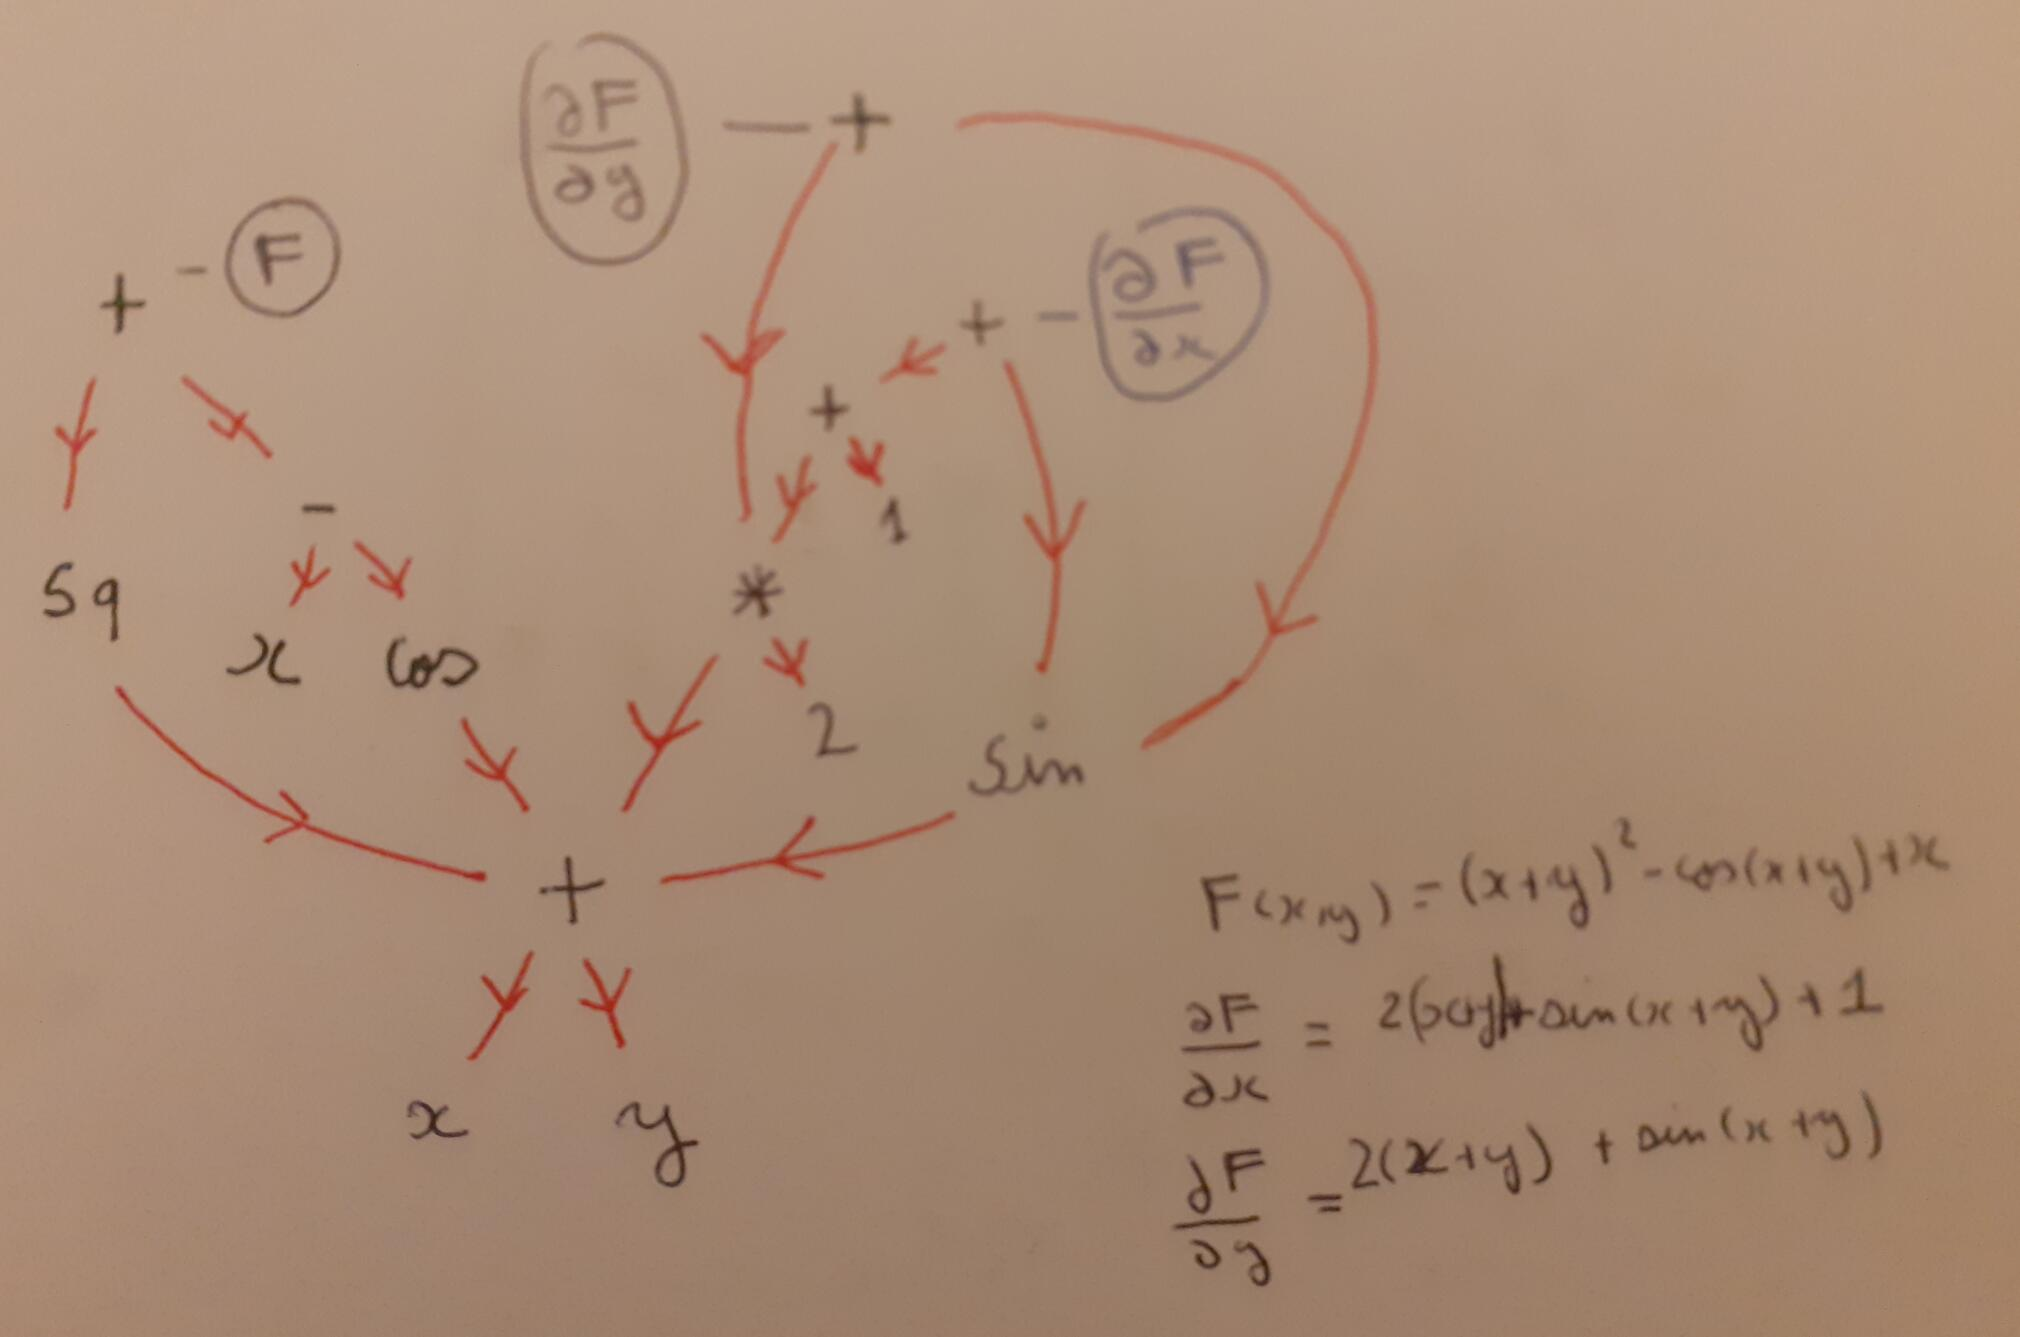
\includegraphics[width=12cm]{Programmer/ImagesProg/DAG.jpg}
\caption{DAG for a multiple formula  $[F,\frac{\partial F}{\partial x}, \frac{\partial F}{\partial y}]$ with $F(x,y) = (x+y)^2 +x - \cos(x+y)$}
\label{fig:DagMultiformula}
\end{figure}


%-----------------------------------------------------
%-----------------------------------------------------
%-----------------------------------------------------

\section{General organization}

%-----------------------------------------------------

The code is located in  {\tt MMVII/include/SymbDer/}.

\subsection{formulas}

The key-file is {\tt SymbolicDerivatives.h}  where is defined   the key-classes   {\tt cFormula and cImplemF},
cFormula being simply pointer on cImplemF,  ({\tt cImplemF} is the real class containing the data, while
{\tt cFormula} are the classes manipulated externally as we want a remanent objet  semantic).
For now we will speak of formula to name undifferrently these two linked classes.


A formula is the {\tt C++} equivalent of the tree/DAG, basically formula work this way :

\begin{itemize}
       \item  a formula contains a set of sub-formula (currently between $0$ en $2$);

       \item  for each kind of formula there is a derived class (i.e one derived class for each operator)

       \item  mathematical operator ($+,*\dots ,\cos,\tan,\dots$) have been overloaded on formula, 
               for example consider a binary operator  $\otimes$ , each time we meet $F_1\otimes F_2$ 
		the rule is to create a new formula of the adequate derived class $c\otimes$ with  
		$\{F_1,F_2\}$ as set of sub-formula,
		there is two (very frequent) exception to this creation of new formula:

               \begin{itemize}
                    \item if the formulla has already be encontered inside a computation, this formula is returned
                          and nothing is created (that why it's a DAG);
		  \item if some simplication rule specific to the operator exist (like $F*1=F$) they are applied;
               \end{itemize}
	       
        \item  a formula contains several virtual methods indicating how to 
               \begin{itemize}
		       \item  compute its value (used in interpreted mode, not usefull for code generation)
		       \item  computes its derivative by return a new formula;
		       \item  computes the generated code;
               \end{itemize}

		the above listing extract these $3$ methods for the {\tt cMulF} correspondingto the multiplication
		of functions;
\end{itemize}


\begin{lstlisting}[language=c++]
// method for computing values
void ComputeBuf(int aK0,int aK1) override
{
    for (int aK=aK0 ; aK<aK1 ; aK++)
        mDataBuf[aK] =  mDataF1[aK] * mDataF2[aK];
}
// === Extract of code in class cMulF (multiplication of formulas )

// method for computing the derivative
cFormula<TypeElem> Derivate(int aK) const override
{
   return  mF2*mF1->Derivate(aK) + mF1*mF2->Derivate(aK);
}

// method for generating the code
std::string GenCodeDef() const override 
{
    return "(" + mF1->GenCodeRef() + " " + this->NameOperator() +  " " + mF2->GenCodeRef() + ")";
}

\end{lstlisting}

%-----------------------------------------------------

\subsection{Coordinator}

Generating the DAG, requires some coordination between the formulas created.
As we want to create a DAG with  minimal number of nodes, we must keep track
of all already existing formulas created for a specific task.
This is where the class {\tt cCoordinatorF} is usefull,  it creates a dictionnary ({\tt std::map})
that stores the association "name/Formula created".  So the coordinator "knows" all the 
formula that belongs to it while each formula "knows" its coordinator. Also the coordinator
associates to each new formula a unique number.

Let illustrate on an example how it works :

\begin{itemize}
	\item  suppose the code contains  $F_1\otimes F_2$  (or  $\otimes(F_1,F_2)$ );
	\item  when this code is executed, $F_1$ and $F_2$ have been created and are given as
		parameter to $\otimes $ (overloaded on formulas), the coordinator has
		attributed a unique number $N_1$ and $N_2$ to these formulas;
	\item  in the function {\tt cGenOperatorBinaire::Generate}, an identifiant is computed $Id="\otimes \; N_1 \; N_2" $,
	\item  if there is a value associated to $Id$, this value is returned, else a new formula is created 
	       the association "Name/formula" is memorized in its coordinator dictionnary, and this new value is returned;
\end{itemize}

The coordinator  is the access point for generating the code. The user has first to select the curent formulas :
it can be the formulas themselves or the formulas plus all their derivatives.
Note that we have the possibility to give several formulas (in a {\tt std::vector}) as curent formulas,
this is because, due to DAG reduction,  the  DAG of $N$ formulas will have less nodes
than the $N$ independant DAG and consequently the code will be more efficient.

Also why would a user generate code without derivatice while
obiously these classes are interesting because we want to compute derivatives? 
In fact  it can be interesting for a given formula to use it both for  computing funcion+derivative and
computing  only the function : for example in weighted least squares, we can whish to first compute the function
only and, if certain conditions are satisfied, compute the derivative.

Once the current formula has been settled, the code generation follows this pipeline :

\begin{itemize}
     \item make a topologicall sort of the formulas that can be reached from the current formulas
         (in topoligical sort a formula appears always after its sons);

     \item generate the code by parsing the sorted formula, the code is pretty monotom with 
           a succession of lines like $V_i = V_j \otimes V_k; $, due to topologicall sort, we are
           sure when this line is generated that $V_j$ and $V_k$ have been initialized;
\end{itemize}


%-----------------------------------------------------

\subsection{class calculator}

Once we have generated the code, we generally want to use it ;-)  that is where 
the class {\tt cCalculator} step in.  The class {\tt cCalculator} is an interface
class that gives access to calculation of generated code.

Basically,  a {\tt cCalculator} is an abstraction of real function,
if we have a formula with $n$ unkonwns that compute $m$ value and their partial derivatives,
the function will be $\RR^n \rightarrow \RR^{(n+1)*m}$. 
The function {\tt DoOneEval} take as parameter two vectors, one for variable and the other
for observations, and return the vector value (of size $(n+1)*m$).

The {\tt cCoordinatorF} inherits of class {\tt cCalculator}, it can  compute the
value of formulas, by the way it's an interpreted mode and is not very efficient.
In the code generated, the class generated also inherit from {\tt cCalculator},  they
use the generated code to compute efficiently the value in {\tt DoOneEval} ,
and they can be manipulated via the unique interface of a {\tt cCalculator}
(in fact in {\tt MMVII}, the "devlopper/user" of this service do not need to load
directly the file generated, he can just get an object from its name).

%-----------------------------------------------------
%-----------------------------------------------------
%-----------------------------------------------------

\section{Classes for  formula}

There exists $3$ main class that derive from the class {\tt cImplemF}, these $3$ classes
correspond to the cases where the formula has $0,1$ or $2$ sub-formula.

      %-----------------------------------------------------
\subsection{Atomic formula}

The atomic formula are the "final" (or "primitive" formula) .  The base
class for them is {\tt cAtomicF}, there is now $3$ atomic derived class, and
probably it will stay like that. The $3$ atomic formula are : 
class for unknowns $x_1,x_2\dots$ ({\tt cUnknownF}), class for constants ({\tt cConstantF}),
and class for observations ({\tt cObservationF}).

It should be pretty obvious what {\tt cUnknownF}  and {\tt cConstantF} represent.
Class {\tt cObservationF} is a less intuitive : consider the equation of 
$2d$ network  where we want to enforce the euclidean distance between $P_1=(x_1,y_1)$ and $P_2=(x_2,y_2)$
to be equal to $D_0$:

\begin{equation}
   d(P_1,P_2) = (x_1-x_2)^2 + (y_1-y_2)^2 = D_0
\end{equation}

In this equation $x_1,y_1,x_2,y_2$ are unknown and, in adjustment, we will need to compute 
the partial derivative relative to them. In the partial derivative $\frac{\partial d}{\partial x_1} = 2*(x_1-x_2)$
the $2$ is a contant we know it's value a time of code generation.

The status of $D_0$ is different, we don't know its value at time of code generation, but a run time
it has a value that will not change because it's not an unknown and for 
any variable $x_k$  we have $\frac{\partial D_0}{\partial x_k} =0$.
$D_0$ can be interpreted as constant whose value will only be fixed at runtime.



      %-----------------------------------------------------
\subsection{Unary formula}

      %  -  -  -  -  -  -  -  -  -  -  -  -  -  -  -  -  -  -  -
\subsubsection{Generatlities}

Unary operator are defined in file {\tt SymbDer/SymbDer\_UnaryOp.h}. Class for implementing unary operator
will derive from class  {\tt cUnaryF}, which itself derive from {\tt cImplemF}.


For definining a new unary operator we will take the example of the square operator   $square : x \rightarrow x^2$.
We must indicate several information, most are located in class {\tt cSquareF}:

\begin{itemize}
	\item   the static method {\tt Operation} simply describes the function itself $x \rightarrow x^2$, it will be  used
		in the reduction rule $ \alpha (C(a)) \rightarrow C(\alpha (a)) $ defined in~\ref{Reduc:Rule};
	
	\item  the static method {\tt StaticNameOperator} return the name of the  operator as a string {\tt "square"}, 
		it is used in code generation and to associate a unique identier to the formula (create an
		identifier like {\tt "square F70"}, where  {\tt "F70"} is the formula with number $70$);

	\item  the method {\tt ComputeBuf} does conceptually same thing as {\tt Operation} , but is used when
		applied to a buffer of data containing several values, (it is used interpretade mode, 
		not for code generation);

	\item  the method {\tt  Derivate}  return \emph{as a formula} the derivate $\frac{\partial F^2}{\partial x_k}$
		of the formula $F$ relatively to variable $x_k$;

        \item note also method {\tt NameOperator} ,it's  a virtual interface to method {\tt StaticNameOperator}
		(the code of this method which will be always the same).
\end{itemize}

Finaly we must also define a operator {\tt square} that work on formula and such that {\tt square(Formula F)} 
return a pointer on a object of type {\tt cSquareF}.  It's a bit more complicated than just creating
the pointer we must :

\begin{itemize}
    \item  check in the coordinator if there is already such formula, and if yes return it;
    \item  else check if  {\tt F} if a constant and if yes apply reduction;
    \item  else create the formula, and indicate to coordinator that it exist.
\end{itemize}

As all this action are systematcic, they can be done in  a generic way, this is done by the class 
template {\tt cGenOperatorUnaire}. So the definition of {\tt square(Formula F)} using this class
is pretty simple :

\begin{lstlisting}[language=c++]
template <class TypeElem> inline cFormula<TypeElem>  square(const cFormula<TypeElem> & aF)
{
    return cGenOperatorUnaire<cSquareF<TypeElem> >::Generate(aF);
}
\end{lstlisting}

      %  -  -  -  -  -  -  -  -  -  -  -  -  -  -  -  -  -  -  -
\subsubsection{Existing operators}

Also it is relatively easy to define new operators usign the scheme of {\tt  square}, a certain number have been
pre-defined :

\begin{itemize}
    \item integer power {\tt square}, {\tt cube},{\tt pow4}, {\tt pow5},{\tt pow6},{\tt pow7},
     \item unitary minus {\tt -};
     \item trigonometric {\tt cos} and  {\tt sin};
     \item {\tt exp} and  {\tt log};
     \item {\tt sqrt}.
\end{itemize}

There is also {\tt pow8} and {\tt pow9}, that for now use the binary {\tt pow};
and finally {\tt powI(Formula,int)} that return one of the following.

      %  -  -  -  -  -  -  -  -  -  -  -  -  -  -  -  -  -  -  -
\subsubsection{New operator in one line with a Macro}

If one takes a look at definition of class of operator, it's obvious that it's quite repetitive;
it should be possible to define new unary operator with minimal additionnal of code.

This is possible using the macro {\tt MACRO\_SD\_DEFINE\_STD\_UNARY\_FUNC\_OP\_DERIVABLE}
defined in {\tt SymbDer\_MACRO.h}.
Do have a differentiable operator on formula, we just need to indicate the name
of the function computing the values, the name of the function computing the derivative,
and the namespace where they are defined.

The easiest is to take the example of sinus-cardinal defined in  {\tt SymbDer\_MACRO.h}.
To define a new operator we need to have a functions on real values that compute $\sinc$ and a function
that compute $\frac{\partial \sinc}{\partial x}$  this is {\tt DerSinC}.  In {\tt MMVII} these function have been
defined in file  {\tt src/UtiMaths/uti\_fonc\_analytique.cpp}. 


\begin{lstlisting}[language=c++]
MACRO_SD_DEFINE_STD_UNARY_FUNC_OP_DERIVABLE(MMVII,sinC,DerSinC)
\end{lstlisting}

This macro does several things :

\begin{itemize}
	\item  declare the existence of operators {\tt sinC} and {\tt DerSinC} that works on formula;

	\item  define the classes  {\tt csinC} and {\tt cDerDinC} that inherits of {\tt cUnaryF};
		note that {\tt csinC}  will call the operator {\tt DerSinC} in method {\tt Derivate},
		while for {\tt cDerDinC}  we make the choice of having no meaningfull derivate
		(its {\tt Derivate} calls the method {\tt UndefinedOperUn};

	\item  declare the operators {\tt sinC} and {\tt DerSinC} , this definition must occurs  after the class
		definition.
\end{itemize}

The macro is pretty simple to use, the price it that it make choices that will not be always pertinent.
For example the choice that {\tt DerSinC} is not itself derivable may not be acceptable.
In this case it is possible to have a finer tuning usign piece by piece the $3$ macro

\begin{lstlisting}[language=c++]
MACRO_SD_DECLARE_STD_UNARY_FUNC_OP
MACRO_SD_DEFINE_STD_cUnaryF
MACRO_SD_DEFINE_STD_UNARY_FUNC_OP
\end{lstlisting}

An example is done in file {\tt src/SymbDerGen/Formulas\_CamStenope.h} with the function
{\tt cosh} and {\tt sinh}  (hyperbolic trigonometric functions).


      %-----------------------------------------------------
\subsection{Binary formula}

The implemantation of binary formula is pretty much the same than the implementation for unary formula,
the main difference being that binary formula contains 2 sub-formula $F_1$ and $F_2$ \dots

The code for is located in {\tt SymbDer\_BinaryOp.h}.  The base class of all binary formula is
{\tt cBinaryF}.  Binary formula have some method that are used exclusively in the reduction process 
as {\tt IsAssociatif},  {\tt IsDistribExt} and {\tt IsDistribExt}  (and probably usefull only
for the $4$ operator $+-*/$, so default value should work for all new binary operator).

There is $5$ binary operators defined in  {\tt SymbDer\_BinaryOp.h} : $+*/-$ and $pow$.

Like with unary operators, {\tt MACRO\_SD\_DEFINE\_STD\_BINARY\_FUNC\_OP\_DERIVABLE}
make possible to create a new binary operator with a single macro.
This macro take one more parameters than unary one, becasuse  we must indicate the two
derivative by each of the parameter to apply the rule :

\begin{equation}
        \frac{\partial (F_1 \otimes F_2)} {\partial x_k} 
     =   \frac{\partial F_1 } {\partial x_k} * \frac{\partial (F_1 \otimes F_2)} {\partial F_1} 
       + \frac{\partial F_2 } {\partial x_k} * \frac{\partial (F_1 \otimes F_2)} {\partial F_2} 
\end{equation}

Examples can be found in {\tt Formulas\_CamStenope.h}.


      %-----------------------------------------------------

\subsection{Reduction rules}

\label{Reduc:Rule}

To have a faster generated code, several reduction rules are used when 
constructing the formulas. Also this may seems anecdotic,
it has a non negligeable  impact on efficiency, as we can see with the equation~\ref{Form:Reduc}
that gives a basic example using, in a first step, blindly the 
rule of automatic derivation and then applying reduction rule .
We have two gains : first $x$ is obviously faster to compute than $0 * (y+2) + x * (1 + 0)$,
and second it increase the likeliness to have code sharing . Note the time to do
these reductions themselve is taken in a "compilation/generation" step and not at execution
(and by the way this compilation time it neglectible).

\begin{equation}
	\frac{\partial(x*(y+2))}{\partial y}
	=  0 * (y+2) + x * (1 + 0)
	\rightarrow x
	\label{Form:Reduc}.
\end{equation}

We give a, non exhaustive, list of these rules, :

\begin{itemize}
     \item  $0*F \rightarrow 0$ ,   $1*F  \rightarrow F$ , $-1*F \rightarrow -F$ (and idem $F*0\dots$);

     \item  $0/F \rightarrow 0$ ;

     \item  $0+F \rightarrow F$ ,   (and idem $F+0\dots$);

     \item  $-(-F) \rightarrow F$ ,  $F_1-(-F_2) \rightarrow F_1+F_2$;

     \item  $F_1*F_2 + F_1*F_3  \rightarrow F_1*(F_2+F_3)$ , $F_1*F_2 - F_1*F_3  \rightarrow F_1*(F_2-F_3)$ , 
     \item  $F_2/F_1 + F_3/F_1  \rightarrow (F_2+F_3)/F1$ ,  $F_2/F_1 - F_3/F_1  \rightarrow (F_2-F_3)/F1$ , 

     \item if  $F_1 > F_2$ then  $F_1 + F_2  \rightarrow F_2 + F_1$ , here the comparison $F_1 > F_2$ 
           is made on numbering, this rules is here favorize merging in DAG creation , any comparison as long
           as it anti-symetric would hold; we just want to avoid that in the same formula $F_1+F_2$ and $F_2+F_1$
	   cannot be merged;
     \item if  $F_1 > F_2$ then  $F_1 * F_2  \rightarrow F_2 * F_1$ 

     \item  $C(a) \otimes C(b) \rightarrow C(a \otimes b) $  where  $C(x)$ design the formula for constant $x$
	     and $\otimes$ is any bynary operator;
     \item  $ \alpha (C(a)) \rightarrow C(\alpha (a)) $  where  $\alpha$ design any unary operator;

\end{itemize}


%-----------------------------------------------------
%-----------------------------------------------------
%-----------------------------------------------------

\section{Code generation}







\chapter{The mapping object}

%---------------------------------------------
%---------------------------------------------
%---------------------------------------------

\section{Introduction}

%---------------------------------------------
%\subsection{Target of mapping objects}

The mapping  are targeted to offer service for object that represent "smooth" mapping
from $\RR^n  \rightarrow  \RR^p$. As an exemple of class naturally derived from mappings used
in photogrammetry we have :

\begin{itemize}
	\item projection $\pi : (x,y,z) \rightarrow (i,j)$ function of an image sensor, as mapping $\RR^3 \rightarrow \RR^2$;

	\item extended projection $\pi_d :  (x,y,z) \leftrightarrow (i,j,d)$ , where $d$ is  the depth,
		as \emph{bijective} mapping of $\RR^3$  ( $\RR^3 \rightarrow  \RR^3$);

	\item distorsion of central perpective camera as  \emph{bijective} mapping of $\RR^2$;

	\item any  transformation  between two geodetic coordinate systems as \emph{bijective}  of  $\RR^3$.

\end{itemize}

The minimal service that a mapping must offer is to define the method $F$ that computes its values.
The kind of services that offers the  mappingi package is :

\begin{itemize}
     \item offer a default method computing the derivative $\frac{\partial F}{\partial x_i}$  using a basic finite differrence ,
           the class can override this default method if has something better to offer;

   \item for $\RR^n \rightarrow \RR^n$ compute the inverse $F^{-1}(v)$ of a given  value using  an iterative method;
           the class can override this default method if has something better to offer;

   \item compute the approximate inverse mapping  of given mapping using some basis of function and a  least square approach;

   \item offer an interface to use generated code of symbolic derivative as a mapping.
\end{itemize}

%---------------------------------------------
%---------------------------------------------
%---------------------------------------------

\section{General organization}

\subsection{Localization}

The declaration of class for mapping are localized in file {\tt include/MMVII\_Mappings.h}.

The definition of these class are located in folder {\tt src/Mappings/}.
As the mapping class are template, there is an explicit instantiation  for
all expected use.



%---------------------------------------------
\subsection{class {\tt cDataMapping}}

         %  -  -  -  -  -  -  -  -  -  -  -  -  -  -
\subsubsection{Templatization}
The base  class of all mappings is {\tt cDataMapping}, its a template class defined by $3$ 
parameters :

\begin{itemize}
    \item {\tt class Type} which is the floatting number type on which all the computation will be made,
          it can be {\tt tREAL4, tREAL8} or {\tt tREAL16} ;  practically it is for now obly used
          with {\tt tREAL8}; by the way some precaution where made to assure that
          the class be intantiated with any complete numeric type in case higher precision woul be required;


    \item {\tt const int DimIn} the dimension of input space;

    \item {\tt const int DimOut} the dimension of output space.
\end{itemize}

         %  -  -  -  -  -  -  -  -  -  -  -  -  -  -
\subsubsection{Values}

The fundamental method that a  mappings must define is  {\tt Value(s)} and it computes the values of 
the function.  Note that there exist two methods :

\begin{itemize}
     \item {\tt Value} that make the computation of single value ;

     \item {\tt Values} that make the computation of vector of values, it can  be used
           if the class has some parallelism option to accelerate the computation.
\end{itemize}

Note that these two virtual methods  have a default implementation : {\tt Value}
is implemented calling {\tt Values},  while {\tt Values} is implemented calling
{\tt Value}.  So obviously, an infinite recursion will occur if none is defined
(BTW it is dynamically detected in debug mode).  The interest being obviously that
in the derived class, it's possible to overload only one to benefit of both.

For {\tt Values} there are two options : 

\begin{itemize}
     \item  one option where the user gives the vector for storing the result;

     \item  one option where the class furnish its own buffer by reference,
            btw the same vector is always returned, so if the user memorize
            the adress, at next call it will be overwritten; so if the vector
            is not used immediately, a copy must be made.
\end{itemize}



         %  -  -  -  -  -  -  -  -  -  -  -  -  -  -
\subsubsection{Jacobian}

The jacobian is computed by returning pair point/Matrix  where point is
the value  and matrix is the  jacobian. This is because generaly when the 
user needs the jacobian he also needs the value, and also when you 
compute the jacobian, you have also computed the value .

Be aware that even if the user make a copy a vector containing results,
due to {\tt MMVII} implementation of matrix (using shared pointer on data),
at next call the jacobian will overwrite the previous call.  In this rare
case, user should call the {\tt Dup} method.

Like {\tt Value} the  class propose default definition of {\tt Jacobian} that user can override.
The users has three option :

\begin{itemize}
      \item  furnish at the construction of object a "small" value that will be used to 
	      compute the derivative by finite difference;  this small value is a point as  the
             meaning of "small" can be different in each dimension;

      \item  furnish a version that compute jacobian for a single point;

      \item  furnish a version that compute jacobian for a vector of  points;
\end{itemize}

We have the same behaviour that with value : version with point, if not overided, calls version
with vector \dots 

Note that using Jacobian, it is possible to compute the affine mapping that is the
differential in a given point. This is done with {\tt Linearize}  (BTW, currently
this is done in derivate class {\tt cDataNxNMapping}, probably to change).


%---------------------------------------------
\subsection{class {\tt cDataBoundedSet}}

This class is used  to represent bounded set of $\RR^n$. A bounded
set $S$ is made  from a box (that's why it is bounded) and a belong function $I$
(virtual method) such that :

\begin{itemize}
	\item if $I(p) >0$  then $p \in S $
	\item if $I(p) <0$  then $p \notin S $
	\item  ideally $I(p) =0$   then $p$ is at the frontier of $S$;
	\item  "ideally" $I$ should be the signed distance to the frontier or a continuous
		growing function of it (but it's not always possible);
\end{itemize}

Bounded set are used in particular in mapping inversion
by least-square to define the set on which inversion must be made. 
They are used also : for clipping a mesh, for computing z-bufer,
for defining the validity domain of a sensor  \dots list will probably grow.
The  different  {\tt cDataBoundedSet} existing now are :

\begin{itemize}
	\item  the box itself;
	\item  the box itself cliped by a sphere;
	\item  the image of a set $S$ by a mapping   $M$, which insideness is $I(M^{-1}(P))$;
	\item  $3d$ masks of {\tt MMV1} encapsulated as  {\tt cDataBoundedSet}.
\end{itemize}



%---------------------------------------------
%---------------------------------------------
%---------------------------------------------

\section{Simple predefinite mappings}


%---------------------------------------------
\subsection{class {\tt cMappingIdentity}}

Sometime it can be usefull to desribe the identity function as a mapping.
For example as an estimation of rough inverse in iterative inversion.

%---------------------------------------------

\subsection{class {\tt cIMElemLinear}}
\subsection{class {\tt cBijAffMapElem}}
\subsection{class {\tt cInvertMappingFromElem}}

%---------------------------------------------
%---------------------------------------------
%---------------------------------------------

\section{Mapping inversion}

\subsection{Class {\tt cDataNxNMapping}}

This class is just a specializion for case where {\tt DimIn==DimOut}. All stuff
related to inversion will inherit from this class.


\subsection{Class {\tt cDataInvertibleMapping}}

This class is the mother class of mapping that are invertible. An invertible
mapping must simply define {\tt Inverse}  or {\tt Inverses} method that compute
the inverse of {\tt Value}.  Like usual, by default {\tt Inverse} calls  {\tt Inverses}
and {\tt Inverses} calls  {\tt Inverse}; so one at least must be defined else an
inifinite recursion will occur.


\subsection{Class {\tt cDataInvertOfMapping}}

When we have a mapping $M$ that is invertible, this class create a mapping $M'$
that contain a pointer on $M$ and such hat  $M'.Val(P) = M.Inv(P)$ and $M'.Inv(P) = M.Val(P)$


\subsection{Class {\tt cDataIterInvertMapping}}

This is here that we begin to really do something \dots

This class offer a concrete computation of the inverse function by iterative gradient method .
Given $Y$, we want to find $X$  such that $F(X)=Y$,  if we have a current "estimation" $X_k$,
we write $F(X_{k+1}) = F(X_k) + \nabla (X_{k+1}-X_k) = Y$ then :

\begin{equation}
	X_{k+1} = X_k + \nabla ^{-1} (Y-F(X_k)) \label{IterGradInv}
\end{equation}

The method starts  from an initial "guess" $X_0$ and iterates equation~\ref{IterGradInv} until some
condition linked to thresholds $\epsilon,N_{iter}$ is reached ($|F(X_k)-Y|<\epsilon$ or $k>N_{iter}$).
This iterative schema require an initialization $X_0$, this is why the constructor take as
argument a mapping named {\tt RoughInv}. For the rough inverse sometime the user
will have information to give a good estimation , in other case identity (or even 
null function) can works well is the mapping is close to a linear form.  For more difficult case,
a convenient solution can be to use the facilities {\tt cComputeMapInverse} describes in~\ref{CompMapInv}
that compute approximate inverse by least square on a given basis of function (it's the method
used for invering distorsion).

\subsection{Class {\tt cDataIIMFromMap}}

This class is just an adaptator to use iterative inversion . Suppose class {\tt cMapSth} exist,
you want to invert it by iterative scheme of  {\tt cDataInvertOfMapping}, but if you cannot
modify {\tt cMapSth}, you cannot make it inherit of {\tt cDataInvertOfMapping}. So you can
use {\tt cDataIIMFromMap}, that owns a pointer on {\tt cMapSth} on inherit of {\tt cDataIterInvertMapping}
to make the inversion.

%---------------------------------------------
%---------------------------------------------
%---------------------------------------------

\section{Least square fitting, and use for inversion}

\section{class {\tt cLeastSqComputeMaps}}

This pure virtual  class can be used to estimate a mapping by least square from a set of samples.
Its most current used, will probably be for estimation of inverse function from direct.
Suppose we have a set of function  $F_1 \dots F_M$ with  $ F_k : \RR^n  \rightarrow  \RR^p$.
We want to estimate $F$ as a linear combination :

\begin{equation}
	F = \sum  a_k  F_k \label{EqMapLsq1}
\end{equation}

We have a set a point $P_1 \dots P_L $ for which we know  the value $Q_l$ such
that $F(P_l) = Q_l$,  then we solve by least square equation~\ref{EqMapLsq2} :

\begin{equation}
	Q_l = \sum  a_k  F_k(P_l)  \label{EqMapLsq2}
\end{equation}

In class  {\tt cLeastSqComputeMaps} there is not explicit description of $F_k$,
instead this is the pure virtual method {\tt ComputeValFuncsBase}, to override,
that must return for a given point $P$ the vector $F_1(P) \dots F_M(P)$.

The method {\tt AddObs(P,Q)}, and its variants, add an equation corresponding to 
equation~\ref{EqMapLsq2}

%---------------------------------------------
\section{class {\tt cComputeMapInverse}}

\label{CompMapInv}

This class use a well known method for computing apprixomate inverse, if
we can compute direct value of $M$, and have a basis $F_1 \dots $
of function for $M^{-1}$, we just have to generate sufficient sample $P_l$
to solve by least square :


\begin{equation}
	P_l =  M^{-1}(M(P_l)) = \sum  a_k  F_k(M(P_l))  \label{EqMapLsq3}
\end{equation}
 
Given a certain maping $M$, a certain basis of function $F_k$ and least square system
described by {\tt cLeastSqComputeMaps}, solving equation~\ref{EqMapLsq3}, is
quite obvious \emph{except} for one issue : how do we generate the $P_l$.
{\tt cComputeMapInverse} offers a solution that is expected to  satisfy most
current case and be easy to use.  The counterpart is that the implementation
is not trivial, so we give some detailed explanation of the algorithm for future maintenance.
The method has been thought specifically to be used in approximate inversion of distorsion.

The first set of parameter the user must specify :

\begin{itemize}
    \item obviously  mapping to inverse $M$ must be furnish, we will call $M'$ the pseudo
          inverse to compute that will satisfy $M'(M(P)) \simeq P$ for all samples we will generate;


    \item the domain $D'$ on which inversion will have to be made, remember we 
          are computing the pseudo inverse, and we cannot expect $M' \circ M = Id$
          on $\RR^n$, so we have to fix domain on which equation~\ref{EqMapLsq3}
          is optimized;

          note that the domain is specified in ouptut coordinates : a point is
          to be selected if $M(P) \in D'$;  it's not sure if this convention we always
          be the best one, at least its convenient for distorsion because the domain
          we want to specify  is  the sensor rectangle (or circle for fish-eye);

    \item  a seed point $P_0$ that is supposed to belong to $D'$  $M(P_0) \in D$;

    \item  a step $S$ for generating a regular greed in input coordinates;

    \item  a threshold $TJ$ on regularity, $TJ<1$, the use of this threshold is to assure
           that the $M$ is bijective on the domain where we do the computation;
           let $J_0$  be the jacobian in $P_0$, we will consider only point $P$
           where the jacobian $J(P)$ is sufficienlty close to $J_0$

\end{itemize}

\begin{equation}
    ||  J(P) J_0^{-1} -Id|| < TJ  \label{EqJacCloseJ0}
\end{equation}


To compute the points,  on a regular grid, we first need to have a majoration
of the box of interest in input coordinate, because we will need to compute an
image to mark the point of this grid . The domain $D$ is a boundet set,
so it is contained in a box $B$, and we use $J_0^{-1}(B)$ as a first estimation,
however as we want to be sure not to omit any point we dilate it by a factor
$\frac{1}{1-TJ}$.




\begin{figure}
\centering
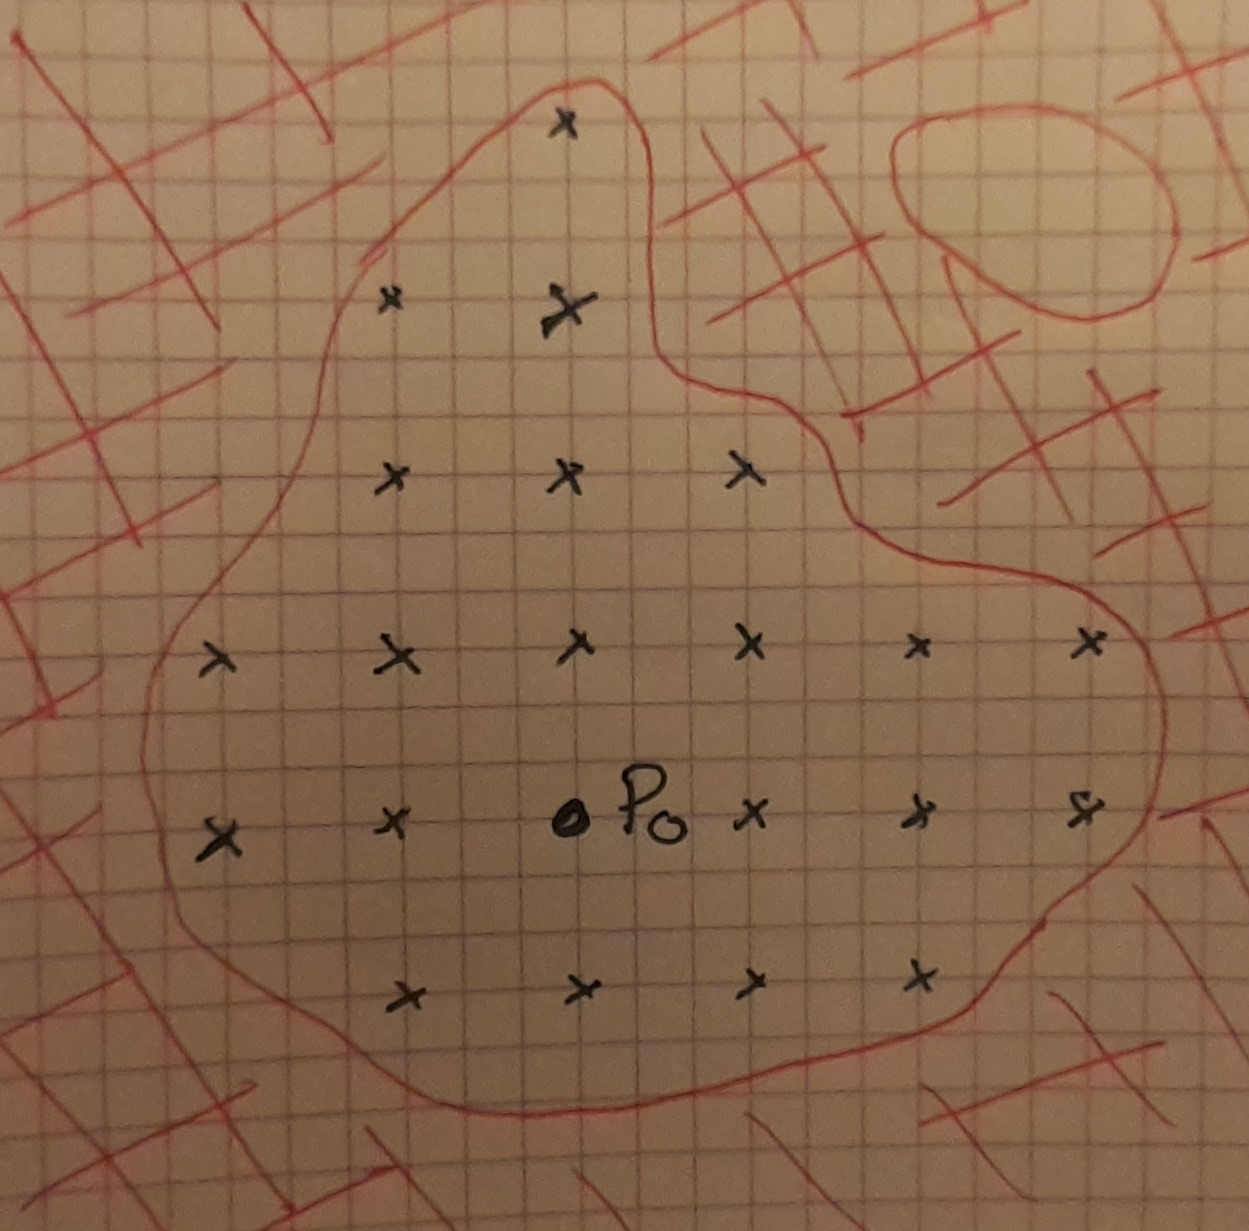
\includegraphics[width=6cm]{Programmer/PointInver-Interior.jpg}
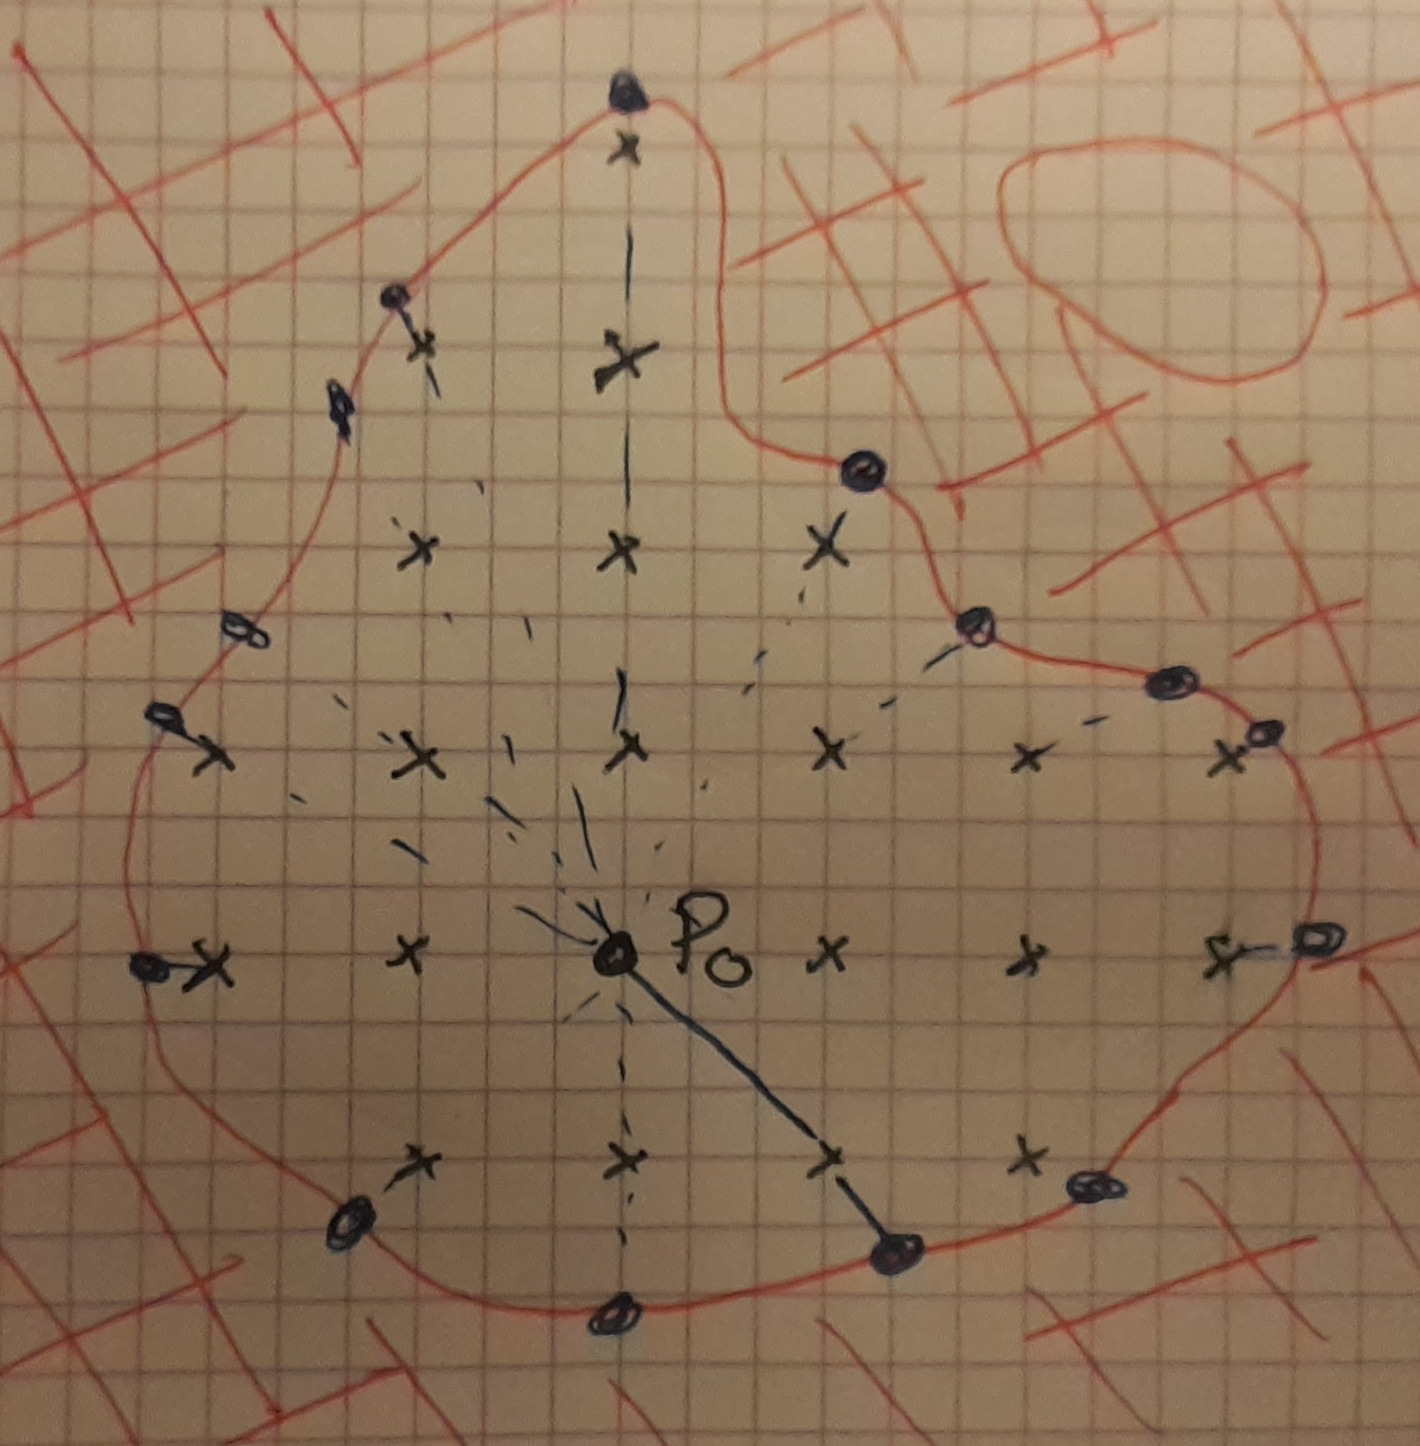
\includegraphics[width=6cm]{Programmer/PointInver-WFront.jpg}
\caption{Generation of sample point for inversion : interior only (left) and with frontier(right)}
\label{fig:PointInvGen}
\end{figure}


Once we have the image, we make a first computation of the "interior" points,
we start from the singleton containing the seed $\{P_0\}$ and compute the connected 
components by iteratively adding the neighboor $P$ respecting equation~\ref{EqJacCloseJ0}
and  $M(P) \in D'$.  This lead to a first set as illustrated by left image 
of figure~\ref{fig:PointInvGen}.

However, this may not be sufficient as we "know" that if computation of such function
is relatively good in interpolation, it can be very unacurate in extrapolation. So there
is a risk that the estimation may be unaccurate close to the frontier; a solution
could be to have a very small step in the grid generation, but this could lead to
a heavy computation.  To overcome this difficulty, we proceed this way :

\begin{itemize}
    \item we select all computed the point on the grid that are that the frontier
          (those who are in $D'$ and  have a neihgboor not belonging to $D'$);

    \item  for each such point $P$,  we use a dicothomic algorithm to prolongate the
	   line $P_0P$ with a point in $D'$ and as close as possible to a point out $D'$,
           this is illustrated by right image of figure~\ref{fig:PointInvGen}.
\end{itemize}


%---------------------------------------------
%---------------------------------------------
%---------------------------------------------

\section{Symbolic derivative \& mappings}

It's often convenient to encapsulate generated code in the class
mappings that offer a higher level description of the same code. 
It's for now the most current case of using mappings.


\subsection{class {\tt cDataMapCalcSymbDer}}

This class embeds two {\tt cCalculator}, one {\tt CVal} for computing
the values, and one {\tt CDer} for computing values and derivatives,
and use them for returning {\tt Values} and {\tt Jacobian}.

There is few restriction on  {\tt CVal} and {\tt CDer}, except that
the number of unkowns is equal to {\tt DimIn} and number of value
returned is equal to {\tt DimOut}.


\subsection{class {\tt cDataNxNMapCalcSymbDer}}

Create a specialization for the case {\tt DimIn == DimOut}.


\subsection{class {\tt cLeastSqCompMapCalcSymb}}

This class use a {\tt cCalculator} for describing a basis of function
that can be used to approximate a funtion (or often its inverse) by least square.

To make it concrete, we anticipate and use the case of basic distorsion, that will be re-explained in 
more detail and more general model in the following chapters. 
Consider a basic model of radial distorsion that integrate a radial distorsion, with
coefficient $k_1,k_2$ and a linear distortion parametrize by $b_1,b_2$. It correspond
to equation~\ref{BasicDist4P}:

\begin{equation}
	D(x,y) =  
	       (1 + k_1 \rho ^2  + k_2  \rho^4)  \begin{pmatrix} x \\ y \end{pmatrix}
	      +   \begin{pmatrix} b_1 x + b_2 y  \\  0 \end{pmatrix}
	\label{BasicDist4P}
\end{equation}

The calculator associated to $D$ will return a formula similar to equation~\ref{BasicDist4P}.
Now we want to compute a pseudo-inverse of $D$, the choice of the basis function will be
a compromise between  the accuracy and the efficiency; basically for accuracy, the more
function the better as long as we avoid degenerency by over-parametrization.
Admit  we make the following reasonnable choice for the basis function  :

\begin{itemize}
    \item  for the radial part, which is generally the most significant,  we need to be accurate;
              also  we take into account the fact that te inverse of a radial function is a radial
              function; in this examplae we take  a radial invers with  $3$ coefficient
              (it's arbitrary, and $2$ or $4$ may be also a good choice, to adapt with the context);

    \item   for the linear part, wich is generally "small", the can restrict ourself to
	    the Taylor expansion $(Id+\epsilon)^1 = Id-\epsilon$, so the functionnal space
            for the inverse is the same that the direct space;
\end{itemize}

So concretely in this example, the functionnal space pseudo invers $D'$  could be given by  :

\begin{equation}
	D'(x,y) =  
	       (1 + k_1 \rho ^2  + k_2  \rho^4 + k_3 \rho^6)  \begin{pmatrix} x \\ y \end{pmatrix}
	      +   \begin{pmatrix} b_1 x + b_2 y  \\  0 \end{pmatrix}
	\label{BasicDistInv5P}
\end{equation}

However , for {\tt MMVII} to be able to separate each of $5$ function  that constitute the basis
of this functionnal space,   $D'$ must not be describe as a sum, conversely we must describe separately
the $10$ coordinate function ($5$ functions of $x,y$) that  constitute the base :

\begin{equation}
	\begin{pmatrix} x \rho ^2 & x \rho ^4  &  x \rho ^6   & x & y \\ 
		        y \rho ^2 & y \rho ^4  &  y \rho ^6   & 0 & 0
       \end{pmatrix}
       =
	\begin{pmatrix} f^1_x &  \dots  & f^5_x  \\
		        f^1_y &  \dots  & f^5_y
       \end{pmatrix}
\end{equation}

In this example, the  {\tt cCalculator} will have to  return  $10$ coordinates as a
vector:
\begin{equation}
    [ f^1_x,  \dots  , f^5_x , f^1_y , \dots, f^5_y]   \label{Vec10Dist}
\end{equation}

Finally, what the class  {\tt cLeastSqCompMapCalcSymb} really does, is takes a
calculator than return a vector similar to~\ref{Vec10Dist} and use it to override
the method {\tt ComputeValFuncsBase}.







\chapter{Photogrammetric organization}


%---------------------------------------------
%---------------------------------------------
%---------------------------------------------

\section{Base class of Sensor {\tt cSensorImage}}

%---------------------------------------------

\subsection{bbb}

          %  - - - - - - - - - - - - - - - - - - - 
\subsubsection{CCC}

%---------------------------------------------
%---------------------------------------------
%---------------------------------------------

\section{Photogrammetric project}



\COM
{
\chapter{The Fits method}

For now "bloc-note",

% Conclusion, on peut sans doute limiter le nombre de point avec ScaleStab
% pour filtrage a priori => genre les 500 les plus stable
}





%---------------------------------------------
%--------------- PART II ----------------------
%---------------------------------------------

\part{Reference documentation}

\chapter{Mesh related commands}


%-----------------------------------------------------------------------
%-----------------------------------------------------------------------
%-----------------------------------------------------------------------

\section{Process of 3D meshes}

 {\tt MMVII} is not a point-cloud/mesh processing tool. However, during some devlopment, some
functionnalities appeared to be necessary and not easily accesible on open source.
As they may be usable in other context I describe them here.

%-----------------------------------------------------------------------
\subsection{MeshCheck}

\begin{verbatim}
 == Mandatory unnamed args : ==
  * string [FDP,Cloud] :: Name of input cloud/mesh
 == Optional named args : ==
  * [Name=Bin] bool :: Generate out in binary format ,[Default=false]
  * [Name=Out] string :: Name of output file if correction are done
  * [Name=Do2DC] bool :: check also as a 2D-triangulation (orientation) ,[Default=false]
  * [Name=Correct] bool :: Do correction, Defaut: Do It Out specified
\end{verbatim}

{\tt MicMac-V1} can generate mesh from a 3d point cloud with normal. For this it
uses the open source tool devlopped by M Kazhdan. Also this tool is robust,
it has sometime topologicall problem that can block further processing.
The command {\tt MeshCheck} has been developped to  detect and potentially
correct these problems.

The first problem detected   is the fact that the same point that is duplicate in
a single triangle  like $ABC$  with $P_A=P_B$. This point are detected and
if the option {\tt Correct} is activated, a graph-quotient algorithm is applied 
on point that are detected as multiple.

The second check is $3d$ surface orientatbility . A message indicating the detected
pair of adjacent triangle badly oriented is printed.  No correction is
done, because untill now no such problem was encounterred.

If the option {\tt Do2DC} is activated, the triangulation is considered
as a $2$ triangle (setting $z$ to $0$) and  the $2d$ orientation correctness is
tested (have all the triangle the same orientation).


%-----------------------------------------------------------------------
\subsection{MeshCloudClip}

\begin{verbatim}
 == Mandatory unnamed args : ==
  * string [FDP,Cloud] :: Name of input cloud/mesh
  * string [3DReg] :: Name of 3D masq

 == Optional named args : ==
  * [Name=Out] string :: Name of output file
  * [Name=Bin] bool :: Generate out in binary format ,[Default=false]
\end{verbatim}


The mesh generated by Poisson method generate a smooth extension of the surface
that can be problematic, for example in the surface devlopment process. This
commande allow to clip the mesh using a $3d$ region.  For now the region
must come in the {\tt MicMac-V1} format as seized by {\tt mm3d SaisieMasqQT}
as for now there is no well established format for $3d$ volumes.
Figure~\ref{fig:MeshClip} illustrate the result of {\tt MeshCloudClip}

\begin{figure}
\centering
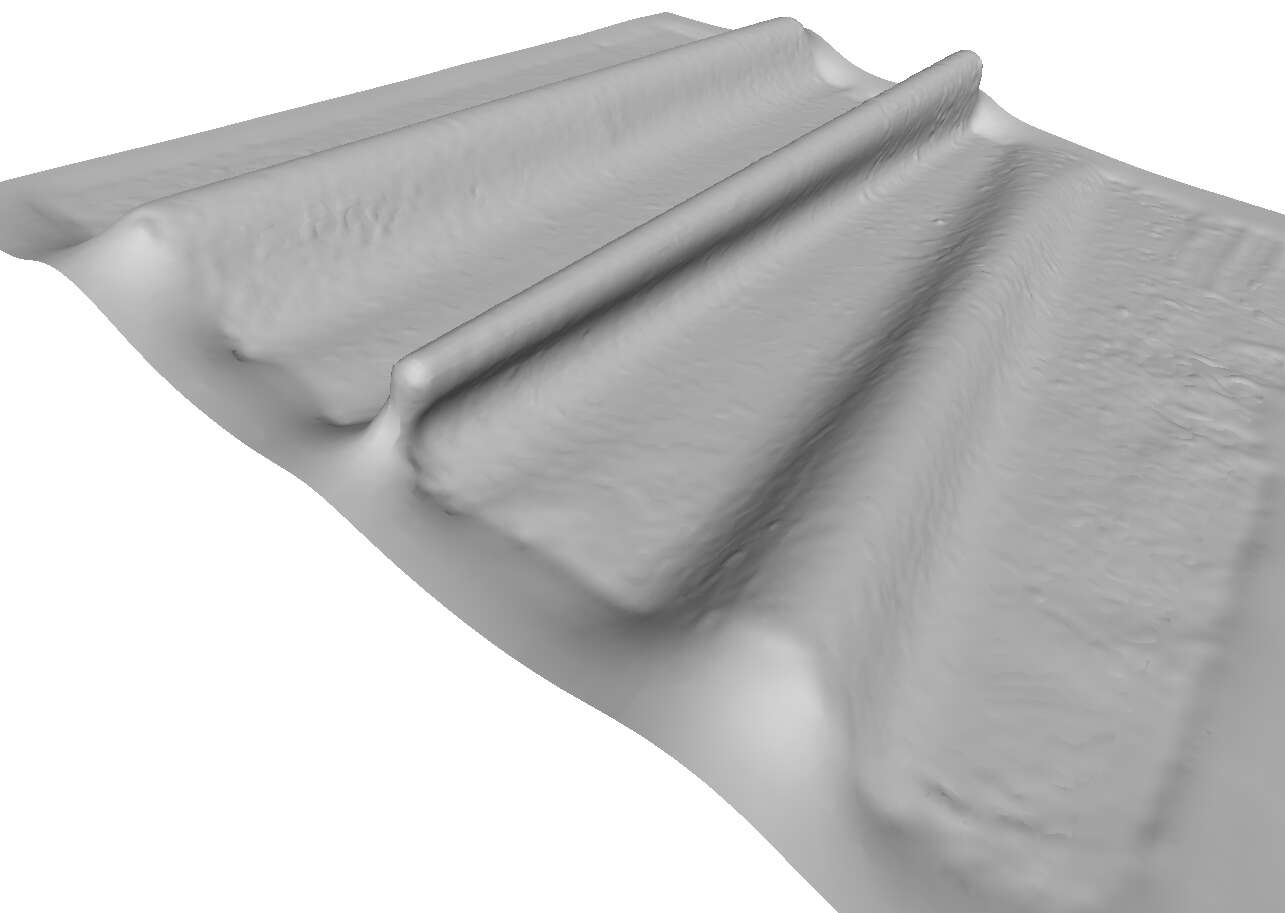
\includegraphics[width=6cm]{CommandReferences/ImagesComRef/MeshWithSkirt.jpg}
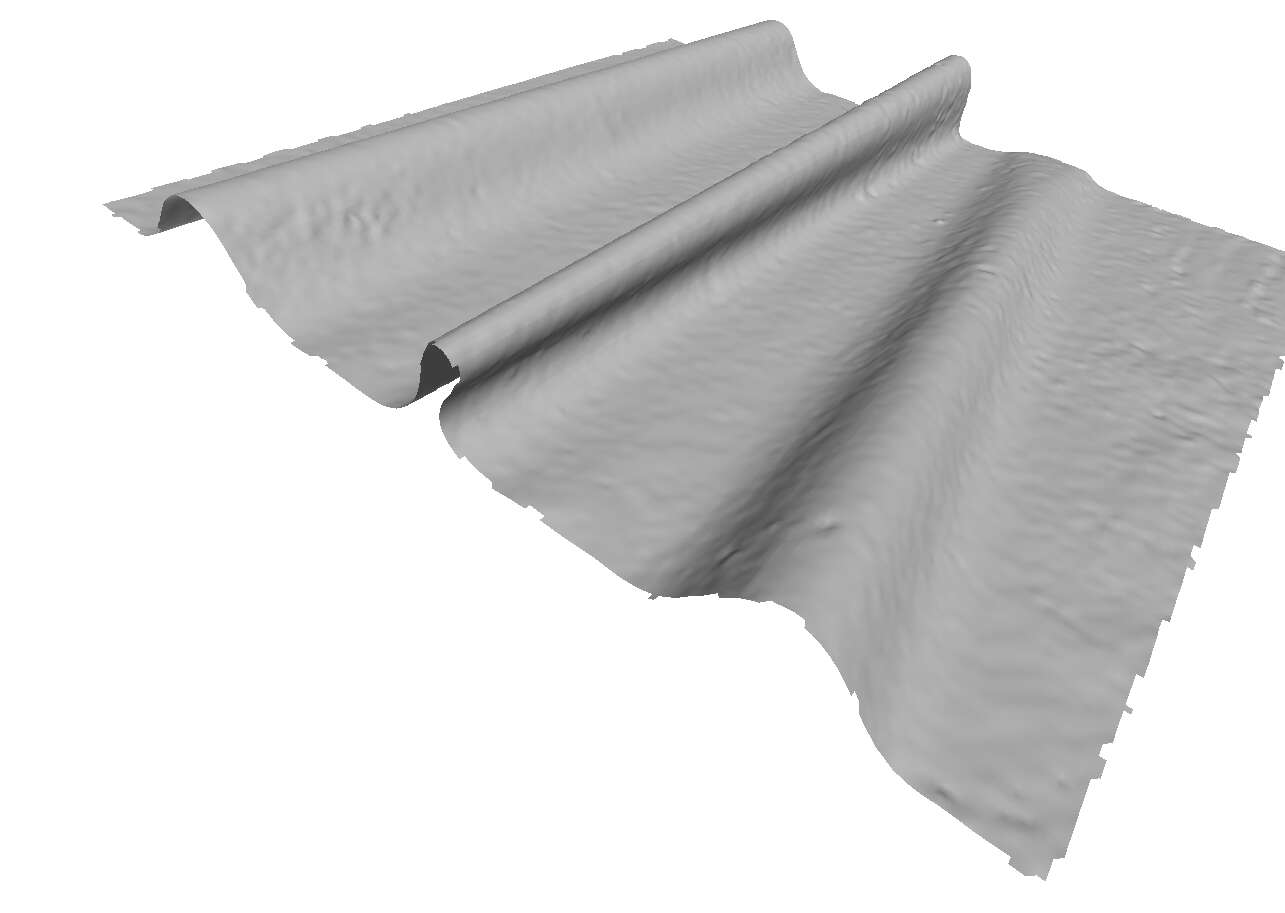
\includegraphics[width=6cm]{CommandReferences/ImagesComRef/MeshCliped.jpg}
\caption{Letft mesh with undesirable extension, right mesh after clipping}
\label{fig:MeshClip}
\end{figure}



%-----------------------------------------------------------------------
%-----------------------------------------------------------------------
%-----------------------------------------------------------------------

\section{Mesh development}

This section describe the tools that were devloped for surface devlopment.

%-----------------------------------------------------------------------
\subsection{MeshDevGen}
This "tiny" tool was made to check the correctness of the surface devlopment algorithm. 
It generate a synthetic mesh, that is completely devlopable and for with we
know the 2 devlopment. This surface is a $3$ extrusion of a logarithmic spiral.

Figure~\ref{fig:SpirAndDev} represent the 3D surface and its developped 2d surface.

\begin{figure}
\centering
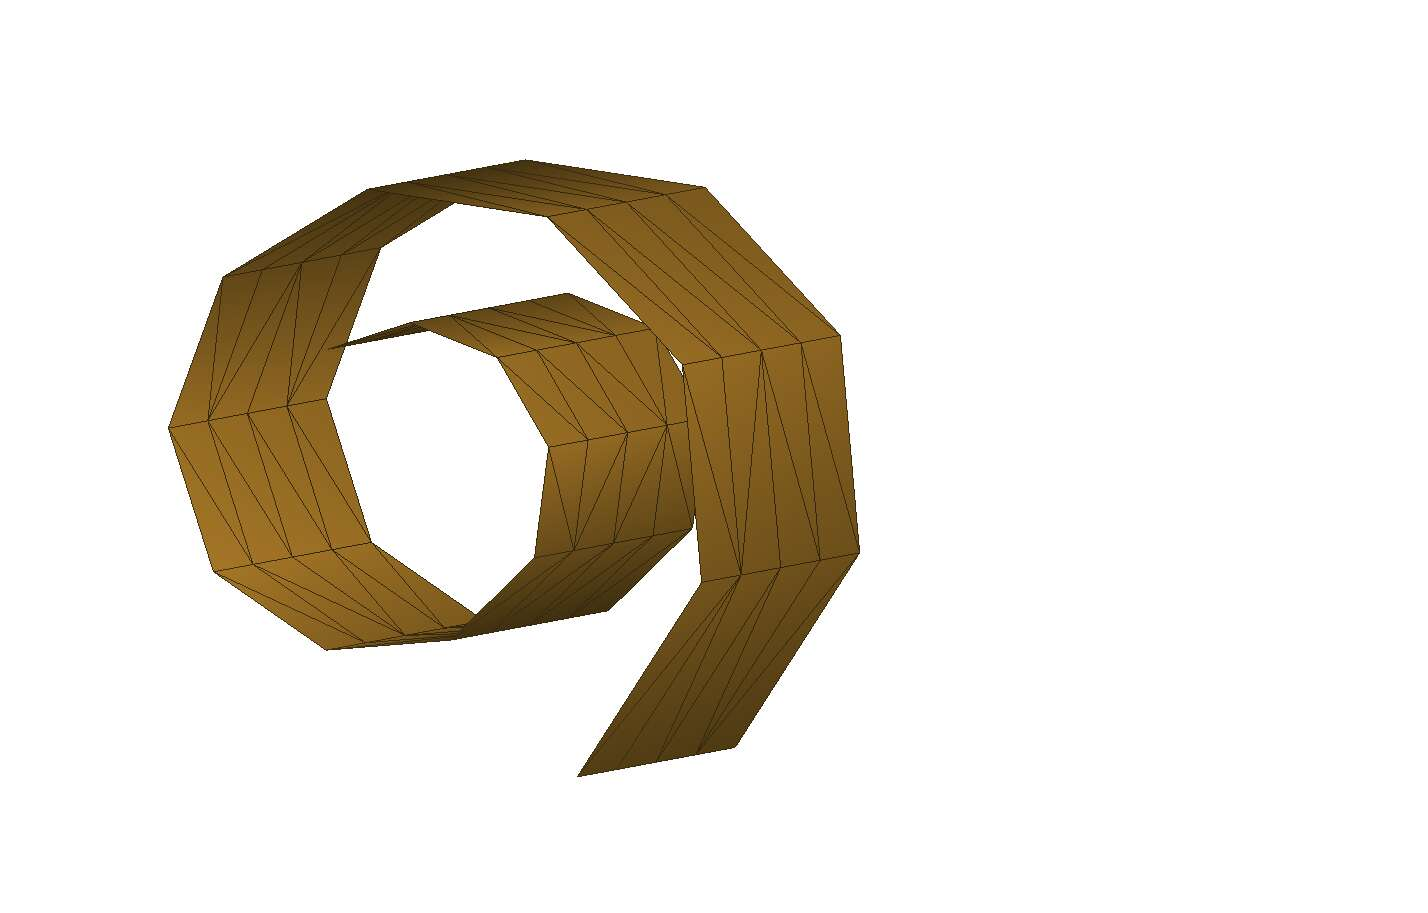
\includegraphics[width=6cm]{CommandReferences/ImagesComRef/Cyl3D01.jpg}
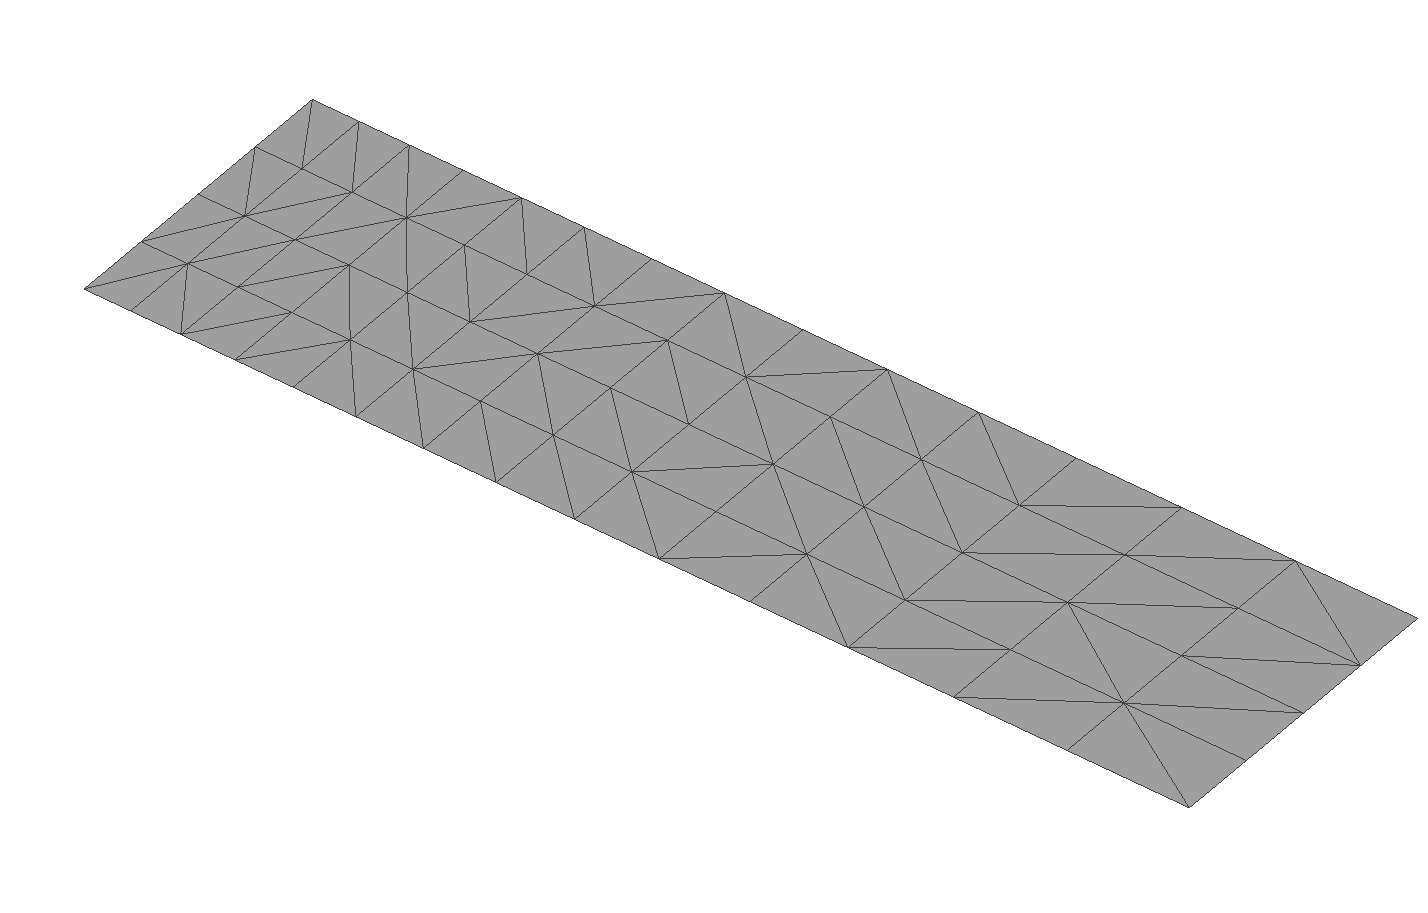
\includegraphics[width=6cm]{CommandReferences/ImagesComRef/CylDev00.jpg}
\caption{A synthetic 3D mesh, and its generated devloped surface}
\label{fig:SpirAndDev}
\end{figure}

%-----------------------------------------------------------------------
\subsection{MeshDev}

\begin{verbatim}
== Mandatory unnamed args : ==
  * string [FDP,Cloud] :: Name of input cloud/mesh
== Optional named args : ==
  * [Name=Out] string :: Name of output file
  * [Name=Bin] bool :: Generate out in binary format ,[Default=false]
  * [Name=NbCByS] int :: Number of compensation by step ,[Default=3]
  * [Name=ShowAv] bool :: Show advancement of computation ,[Default=true]
  * [Name=CheckReach] bool :: Check reached face&som at end ,[Default=true]
  * [Name=WDistE] double :: Weight on edge dist ,[Default=0]
  * [Name=WRot] double :: Weight on rot on 2d triangles ,[Default=1]
  * [Name=NbIE] int :: Number of iteration at end
\end{verbatim}

\begin{figure}
\centering
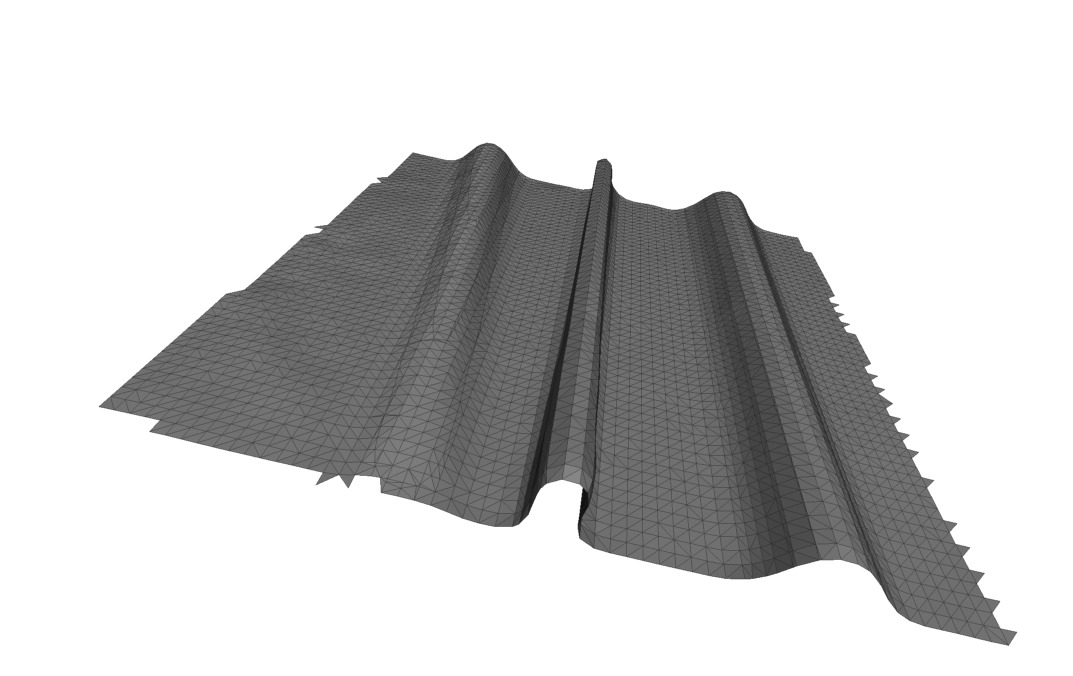
\includegraphics[width=6cm]{CommandReferences/ImagesComRef/Mesh3D.jpg}
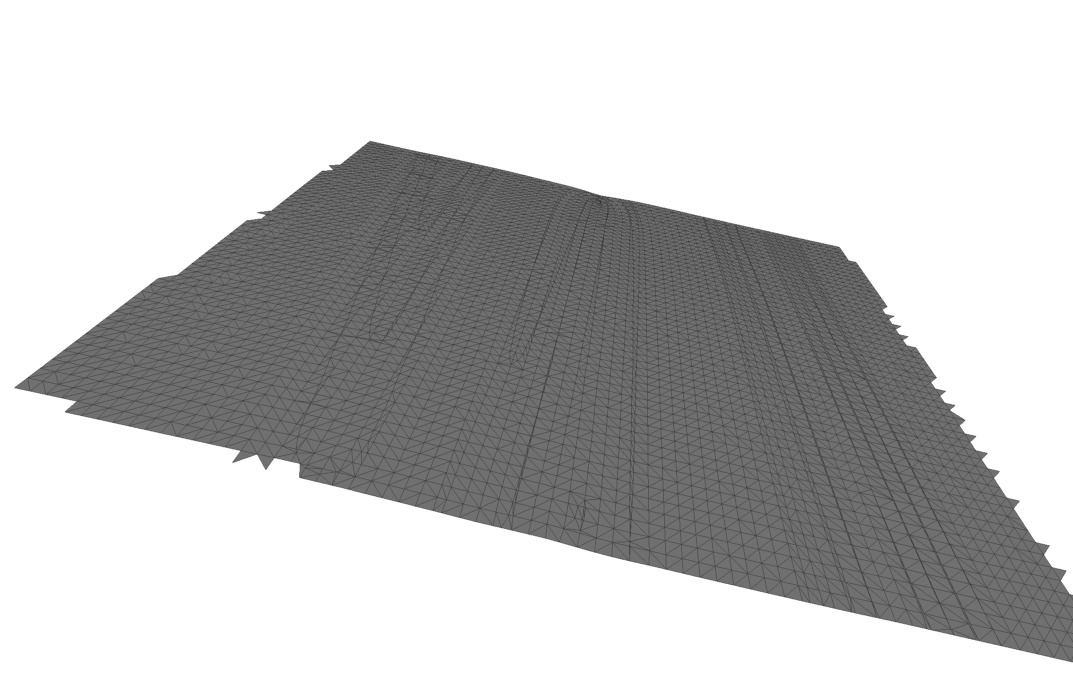
\includegraphics[width=6cm]{CommandReferences/ImagesComRef/Mesh2D.jpg}
\caption{A "real" mesh and its devlopment after MeshDev}
\label{fig:RealDev}
\end{figure}


This tool is used to make the $2d$ development of a $3d$ surface. As the real surface
is generally not strictly devlopable, this is done by minimzing the energy of deformation.
Figure~\ref{fig:RealDev} presents a $3d$ mesh and its $2d$ devlopment.
The constraint is that the devlopment must be, as much as possible isometric (distance on
the plane is the same that geodetic distance on $3d$ surface).  More precisely :

\begin{itemize}
      \item let  $P_i$ be the $3d$ points of the triangulation, $P_i \in \RR^3$;
      \item let  $\phi(P_i)$ be unknown $2d$  position of the devlopment $\phi(P_i) \in \RR^2$;
      \item let  $\mathcal{T}_t = \{P_{t_1},P_{t_2},P_{t_3}\}, t \in [1,T] $ be the $T$ triangles;
\end{itemize}


The command offers different option corresponding to different formalization of the isometry.
The simpler is given by :

\begin{equation}
   E_d(\phi) =   \sum_{t=1}^T \sum_{m,n=1}^3  \{ d(P_{t_m},P_{t_m})-  d(\phi(P_{t_m}),\phi(P_{t_m})) \}  ^2
   \label{DevEqDist}
\end{equation}

For technicall reason (see paper to come) the equation~\ref{DevEqDist} is not stable and
the equation~\ref{Eq:MeshDev1T} is generally preferable.
For each triangle  $\mathcal{T}_t$ \emph{independantly} we can easily compute a \emph{perfect} development
in a $2d$ triangle $\mathcal{T}^2_k$= $q_{t_1},q_{t_2},q_{t_3}$, such that 
$d(q_{t_n},q_{t_m})=d(P_{t_m},P_{t_n}) \; m,n \in (1,2,3)$, so if the development
were perfect, there would exist for each triangle a rotation $R^t$ such that :

\begin{equation}
	\phi(P_{t_m}) =  R^t q^t_m  \;\; m \in (1,2,3) \label{Eq:MeshDev1T}
\end{equation}


Let note $\psi$ the application associate a rotation to each triangle $R^t = \psi(\mathcal{T}_t)=$.
We then try to compute simultaneously the $\phi$ and $\psi$ that minizes globaly the 
formula of equation~\ref{Eq:MeshDev1T} :

\begin{equation}
    E_R(\phi,\psi)= \sum_{t=1}^T \sum_{m=1}^3  d\{\phi(P_{t_m}) - \psi(\mathcal{T}_t)(q_{t_m})\} ^2
\end{equation}

%-----------------------------------------------------------------------

\subsection{MeshProjImage}

\subsubsection{General use}

\begin{verbatim}
 == Mandatory unnamed args : ==
  * string [MPF0,FDP] :: Name of image
  * string [Cloud,In] :: Name of input cloud/mesh
  * string [Ori,In] :: Input Ori
  * string [MeshDev,Out] :: Output MeshDev
 == Optional named args : ==
  * [Name=M2] string [Cloud,In] :: Mesh 2D, dev of cloud 3D,to generate a visu of hiden part
  * [Name=ResZBuf] double :: Resolution of ZBuffer ,[Default=3]
  * [Name=DoIm] bool :: Do images ,[Default=false]
  * [Name=NbPixIR] int :: Resolution of ZBuffer ,[Default=2000]
  * [Name=MII] double :: Margin Inside Image (for triangle validation) ,[Default=4]
  * [Name=SkWE] bool :: Skip command when result exist
  * [Name=OutRad] string [Rad,Out] :: Output Rad
  * [Name=FFI0] string [FFI0] :: File Filter Interval, Main Set
\end{verbatim}

This command is used to prepare the image devlopment taking into account the orientation of the
camera and a $3$ surface.  It must decides for each triangle, which is the best image to
use for creating textures . For each image and each triangle, the method :

\begin{itemize}
    \item decide if the triangle is visible, this is done copmputing a ZBuffer;
    \item for a visible triangle, computes the resolution (precisely the lowest resolution 
          on all the possible direction);
\end{itemize}

Finally the  command select for each triangle the image having the best resolution among the images where
the triangle is visible.

\begin{figure}
\centering
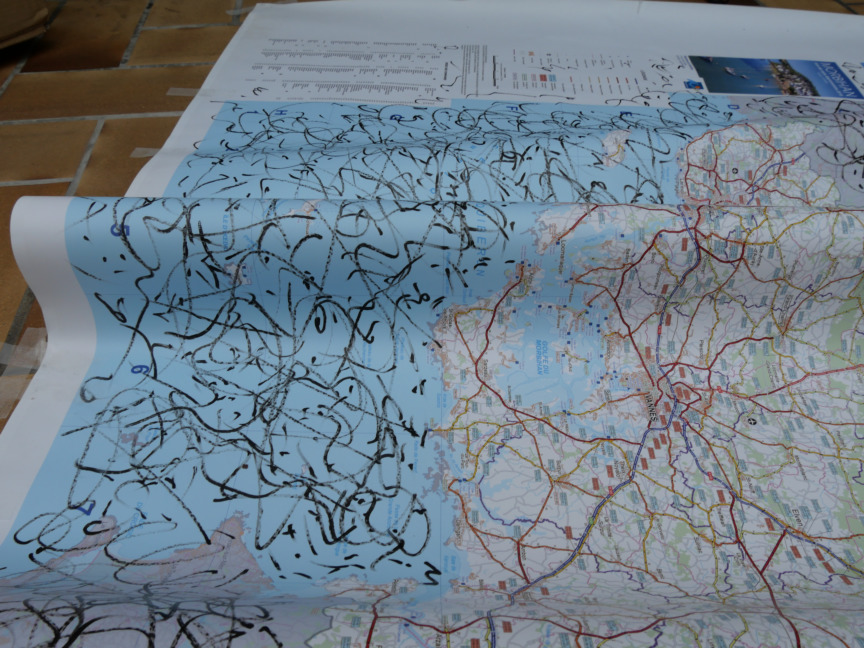
\includegraphics[width=6cm]{CommandReferences/ImagesComRef/Image_P1056148.jpg}

\includegraphics[width=6cm]{CommandReferences/ImagesComRef/ZBuf.jpg}
\caption{An image , the ZBuffer computed,the view on devloped mesh of visibility and resolution}
\label{fig:RealDevZB}
\end{figure}

The figure~\ref{fig:RealDevZB} presents some intermediar result computed during
this commande.  The left image is just the image used to illustrate the computation,
the right image is the zbuf computed, by default this z-buffer is not saved as it is
just an intermediar of computation, if wanted for illusration the {\tt DoIm=true} activates that.

\begin{figure}
\centering
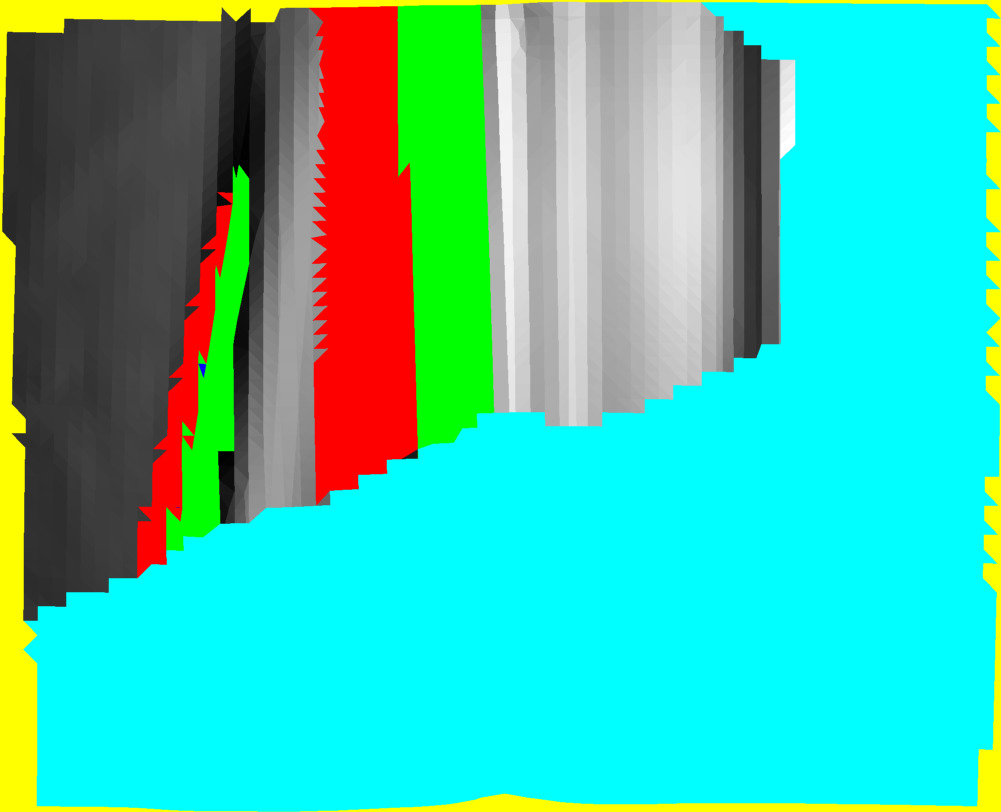
\includegraphics[width=6cm]{CommandReferences/ImagesComRef/Dev-P1056148.jpg}
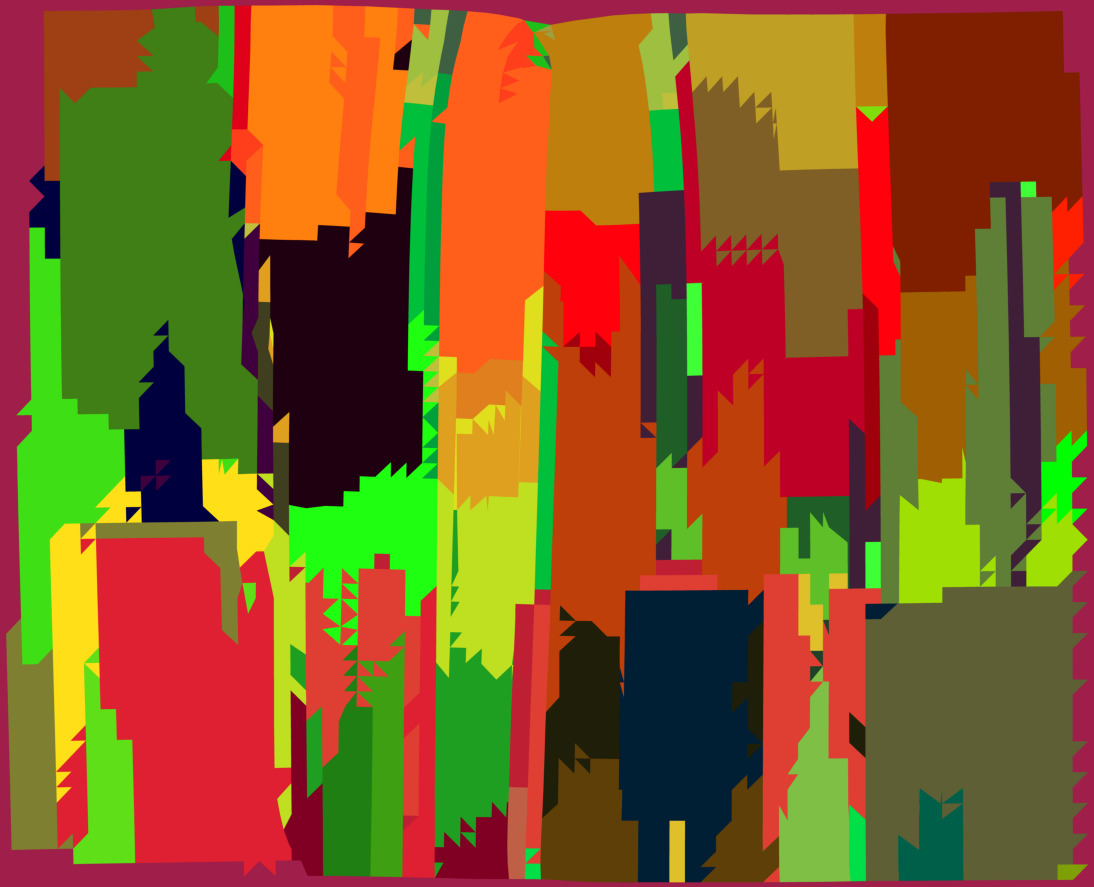
\includegraphics[width=6cm]{CommandReferences/ImagesComRef/LabTri.jpg}
\caption{Left visibility an resolution for $1$ image, right visualisation of selected triangle}
\label{fig:RealDevTri}
\end{figure}

The figure~\ref{fig:RealDevTri} presents the result of computation, these two images are in the
geometry of devlopped $2d$ surface :

\begin{itemize}
    \item left  image present the visiblity of triangle , gray triangle are visible and the gray value is
          proportionnal to the computed resolution; cyan correspond to background (no triangle or triangle
          dont project in image),  red present triangle that are correctly oriented but occluded by others,
          green present the triangle that cannot be visible due to their orientation;

    \item right image present the result of best triangle selection using a random palette (same color
          visualize triangles affected to the same image;

\end{itemize}

     %  -  -  -  -  -  -  -  -  -  -  -  -  -  -  -  -  -  -  -  -  -  -  -  -

\subsubsection{Radiometry computation}

An important option of the command is {\tt OurRad},  if used it will generate in
the specifying folder data that can be used for radiometric equalization (see
chapter \ref{Chap:Radiom} for structures of such data). Some details :

\begin{itemize}
    \item each $3d$ triangle is sampled on a grid , each of this point 

\end{itemize}



\subsubsection{Result}

The results are stored in a folder computed from the $4^{th}$ parameter.



%-----------------------------------------------------------------------
\subsection{MeshImageDevlp}

\begin{verbatim}
== Mandatory unnamed args : ==
  * string [FDP] :: Name of 2d devloped mesh
  * string [MeshDev,In] :: Input MeshDev
 == Optional named args : ==
  * [Name=WGL] bool :: With Gray Label 2-byte image generation ,[Default=false]
  * [Name=WRGBL] bool :: With RGB Label  1 chanel-label/2 label contrast ,[Default=false]
  * [Name=InRad] string [Rad,In] :: Input Rad
\end{verbatim}

This command is used for computing effectively the $2d$ devlopment of the image . Its takes two mandatory
parameters :

\begin{itemize}
   \item the $2d$ mesh as resulting from the command {\tt MeshDev};
   \item the folder containing the result of {\tt MeshProjImage};
\end{itemize}

If the images are to be equalized before devlopment, The optionnal parameter {\tt InRad} 
indicate where the radiometric equalization data can be found.  

The parameter {\tt WGL} and {\tt WRGBL} can be used to generate visualization as the one
of figure~\ref{fig:RealDevTri}, except for didactic or debugging, they will be generally not usefull.
 With {\tt WGL} a gray level- $16$ bits- image is generated,
each level indicating the id of the triangle. With {\tt WRGBL}, a rgb-$8$ bits- image is generated, the 
blue channel indicate the num of the triangle, while red and green channel are selected to maximize
the contrast.





%---------------------------------------------
%--------------- PART I ----------------------
%---------------------------------------------

\part{Annexes}

\appendix

\chapter{Bibliography}


\begin{thebibliography}{AAA}
   \bibitem[Tomasi Kanabe 98]{TomKan}   S. Roy, I.J. Cox , 1998, "Shape and Motion from Image 
            Streams under Orthography: a Factorization Method", International Journal of Computer Vision, 
            9:2, 137-154 (1992)


    \bibitem[CERES]{CERES} \emph{https://github.com/ceres-solver/ceres-solver/blob/master/include/ceres/jet.h}

   \bibitem[Cox-Roy 98]{CoxRoy}   S. Roy, I.J. Cox , 1998, "A Maximum-Flow
            formulation of the N-camera Stereo Correspondence
      Problem", \emph{Proc. IEEE Internation Conference on
      Computer Vision}, pp 492--499, Bombay.

   \bibitem[Fraser C. 97]{Fraser}  C. Fraser, 1997, "Digital camera self-calibration",
   \emph{ISPRS Journal of Photogrammetry and Remote Sensing}, vol. 52, issue 4, pp. 149-159,
   \bibitem[Penard L. 2006 ]{Penard}   L. Pénard, N. Paparoditis, M. Pierrot-Deseilligny.
           "Reconstruction 3D automatique de façades de bâtiments en multi-vues.",
            RFIA (Reconnaissance des Formes et Intelligence Artificielle),
            Tours, France, January 2006.

    \bibitem[Weierstrass,Karl 1885 ]{Weierstrass1885} Über die analytische Darstellbarkeit sogenannter willkürlicher Functionen
           einer reellen Veränderlichen. Sitzungsberichte der Königlich Preußischen Akademie der Wissenschaften zu Berlin,
           1885 (II).  Erste Mitteilung (part 1) pp. 633–639, Zweite Mitteilung (part 2) pp. 789–805.

    \bibitem[Stone, M. H. 1937]{Stone1937} "Applications of the Theory of Boolean Rings to General Topology",
          Transactions of the American Mathematical Society, Transactions of the American Mathematical Society,
          Vol. 41, No. 3, 41 (3): 375–481

\end{thebibliography}


\printindex



\end{document}




